%% Vorlage HTBL Hollabrunn Diplomarbeit
%% KOMA Script
\documentclass[12pt,ngerman,a4paper,parskip,twoside,listof=totoc,tikz]{scrartcl}

\usepackage{hhline}     % Tutorial Table border
\usepackage{listings}   % Code Listings
\usepackage{lstlangarm} % ARM ASM

\lstset{
    language=C,
    basicstyle=\ttfamily,
    keywordstyle=\color{blue}\ttfamily,
    stringstyle=\color{red}\ttfamily,
    commentstyle=\color{green}\ttfamily,
    morecomment=[l][\color{magenta}]{\#},
    basicstyle=\footnotesize,
    numbers=left,
    stepnumber=1,
    showstringspaces=false,
    tabsize=1,
    breaklines=true,
    breakatwhitespace=false,
}

\lstset{
    language=[ARM]Assembler,
    basicstyle=\ttfamily,
    keywordstyle=\color{blue}\ttfamily,
    stringstyle=\color{red}\ttfamily,
    commentstyle=\color{green}\ttfamily,
    morecomment=[l][\color{magenta}]{\#},
    basicstyle=\footnotesize,
    numbers=left,
    stepnumber=1,
    showstringspaces=false,
    tabsize=1,
    breaklines=true,
    breakatwhitespace=false,
}

\lstset{
    language=XML,
    basicstyle=\ttfamily,
    keywordstyle=\color{blue}\ttfamily,
    stringstyle=\color{red}\ttfamily,
    commentstyle=\color{green}\ttfamily,
    morecomment=[l][\color{magenta}]{\#},
    basicstyle=\footnotesize,
    numbers=left,
    stepnumber=1,
    showstringspaces=false,
    tabsize=1,
    breaklines=true,
    breakatwhitespace=false,
}

\usepackage{hyperref}
\usepackage[ngerman]{babel}
\usepackage[german]{fancyref}

\usepackage{htlDT}    % HTBL Diplomarbeitsstyle

\usepackage{todonotes}

%%%%%%%%%%%%%%%%%%%%%%%%%%%%%%%%%%%%%%%%%%%%%%%%%%%%%%%%%%%%%%%%%%%%%%%%%%%%%%%%%%%%%%%%%%%%% General Settings, like Title, Students and supporters
\title{Advanced Microcontroller Training System}
\student{Andreas Mieke}{Software ARM Cortex-M3 Minimalsystem}{5BHEL}{Dipl.-Ing. Josef Reisinger}
\student{Andreas Reischl}{Z80 Minimalsystem}{5AHEL}{Dipl.-Ing. Josef Reisinger}
\student{Kevin Schuh}{Hardware ARM Cortex-M3 Minimalsystem}{5BHEL}{Dipl.-Ing. Josef Reisinger}
\termyear{2017/18}
\class{5xHEL}
\keywords{ST-Link V2\\ULINK/ME\\Cortex-M3\\\gls{cpu}\\Nextion NX4832T035\_011\\JTAG\\SPI\\UART\\I$^2$C\\\gls{Core-Modul}\\\gls{Basisplatine}\\\gls{USB-to-UART}\\Altium\\$\mu$Vision 5\\ARM}
\sthanks{
    Im Vorhinein möchten wir uns herzlichst bei unserem Diplomarbeitsbetreuer Herrn Dipl.-Ing. Josef Reisinger bedanken, der uns stets kompetent beraten hat und uns sein Wissen zur Verfügung stellte.

    Des Weiterem möchten wir uns bei Herrn Dipl.-Ing. Erwin Dobart bedanken, der uns bei technischen Fragen unterstützte. 
    
    Weiters möchten wir uns bei Herrn FOL StR Ing. Manfred Resel bedanken, der uns, solange er noch im Dienst war, bei Softwareproblemen und Hardwarefragen aller Art zur Seite stand. 
    
    Darüber hinaus möchten wir uns bei Herrn Wolfgang Kauer und Herrn Ferdinand Klampfer bedanken, ohne deren Hilfe wir unsere Leiterkarten nicht hätten bestücken können.
    
    Ebenfalls möchten wir Herrn Dipl.-Ing. Wilfried Trollmann bedanken, welcher uns immer an unsere Fristen und Termine erinnerte und uns jederzeit über aktuelle Wettbewerbe informierte.
    
    Außerdem möchten wir uns bei Thomas Fehringer, unseren Laboranten, bedanken, welcher uns mit Bauteilen für unsere Diplomarbeit versorgte.
}

\aufgabenstellung{Aufgabe soll es sein, eine neue Version für das HTL eigene ARM Minimalsystem zu realisieren. Zunächst soll ein Touchscreen-Display zur Ein- und Ausgabe unterstützt werden. Des Weiteren soll eine Arduino-UNO kompatible Schnittstelle zur Verfügung gestellt werden, um Arduino Shields von verschiedenen Herstellern einsetzen zu können. Darüber hinaus soll das neue System verschiedene Funkmodule unterstützen, um damit eine Kommunikation mit anderer Peripherie zu erleichtern. Ein Audiomodul, welches bereits bei einer Diplomarbeit aus dem Jahre 2015/16 entwickelt wurde, soll ebenso unterstützt werden. Zusätzlich soll noch ein Z80 Minimalsystem, welches im Rahmen mehrerer Diplomarbeiten entstanden ist, für den Einsatz im Laborunterricht vervollständigt werden.}

\realisierung{Zuerst sollen die einzelnen Arbeitsaufträge entwickelt und überprüft werden. Anschließend sollen die einzelnen Systemkomponenten zum fertigen System zusammengefügt und in Betrieb genommen werden. Die Funktion und die einzelnen Entwicklungsschritte zum fertigen Prototypen sollen anschließend durch eine umfangreiche Dokumentation und eine Bedienungsanleitung vervollständigt werden.}

\ergebnisse{Es wurden funktionsfähige Prototypen aller Leiterkarten gefertigt. Darüber hinaus wurde eine Testsoftware zur Überprüfung der Prototypen geschrieben.}

\wettbewerbe{Jugend Innovativ\\Technik fürs Leben-Preis}



\tasks{The task should be to realize a new version for the HTL (secondary technical college) own ARM minimal system. At first, a touchscreen display for input and output should be supported. Furthermore, an Arduino-UNO compatible interface should make it possible to use Arduino shields from different manufacturers.  In addition, the new system should support various wireless modules to facilitate communication with other peripherals. An audio module, which was already developed in a diploma thesis from the year 2015/16, should also be supported. In addition, a Z80 minimal system, which was created in the context of several diploma theses, should be finalised for the use in laboratory lessons.}

\realisation{At first, the individual work orders should be developed and checked. Subsequently, the individual system components were to be assembled into the finished system and put into operation. The function and the individual development steps for the finished prototype should be completed with a documentation and a user manual.}

\results{Working prototypes of all printed circuit boards have been developed. Moreover, a test software to prove the functionality of the prototype has been written.}

\competitions{Jugend Innovativ\\Technik fürs Leben-Preis}

%%%%%%%%%%%%%%%%%%%%%%%%%%%%%%%%%%%%%%%%%%%%%%%%%%%%%%%%%%%%%%%%%%%%%%%%%%%%%%%%%%%%%%%%%%%%% Bibliography
\usepackage[backend=bibtex, style=ieee, citestyle=ieee, hyperref=true]{biblatex}
\makeatletter
\def\blx@maxline{77}
\makeatother

\usepackage{xpatch}
\makeatletter 
\xpatchcmd\blx@head@bibliography{\markboth}{\@mkboth}{}{\undefined} 
\makeatother

\addbibresource{literatur.bib}

%%%%%%%%%%%%%%%%%%%%%%%%%%%%%%%%%%%%%%%%%%%%%%%%%%%%%%%%%%%%%%%%%%%%%%%%%%%%%%%%%%%%%%%%%%%%% Gloassaries
\usepackage[nomain,acronym,toc,section]{glossaries}
\makeglossaries
\makeindex

\usepackage{xparse}
\DeclareDocumentCommand{\newdualentry}{ O{} O{} m m m m } {
  \newglossaryentry{gls-#3}{name={#5},text={#5\glsadd{#3}},
    description={#6},#1
  }
  \makeglossaries
  \newacronym[see={[Siehe:]{gls-#3}},#2]{#3}{#4}{#5\glsadd{gls-#3}}
}
% Usage: \newdualentry{ref}{short}{long}{description}

%%%%%%%%%%%%%%%%%%%%%%%%%%%%%%%%%%%%%%%%%%%%%%%%%% Acronyms
\newdualentry{IDE}{IDE}{integrierte Entwicklungsumgebung}{ist Deutsch für \enquote{Integrated Development Environment} und beschreibt eine Sammlung von Programmen (Editor, Compiler, Linker, Loader, Debugger), welche zum programmieren verwendet wird \cite{wiki:IDE}}

\newdualentry{ARM}{ARM}{ARM Limited}{früher: Advanced RISC Machines Ltd. ist ein zur japanischen Firma Softbank gehörender Hersteller von IP (Intellectual property) Software im Bereich Mikroprozessoren. Die gleichnamige Mikroprozessorarchitektur, ARM, ist zur Zeit weltweit am weitesten verbreitet \cite{wiki:ARM} \cite{techradar:ARM}}

\newdualentry{CMSIS}{CMSIS}{Cortex Microcontroller Software Interface Standard}{ist ein von \gls{ARM} erstellter Standard, welcher das Verwenden von Software zwischen verschiedenen Cortex-Prozessoren verschiedener Chip-Hersteller ohne große Anpassungen ermöglichen soll. Hierfür stellt \gls{ARM} einige Definitionen -- wie zum Beispiel CORE, RTOS, DSP, \dots{} -- zur Verfügung, welche von den Chip-Herstellern implementiert werden, diese stellen dann CMSIS-Packs zur Verfügung, welche in Softwareprojekte eingebunden werden können. Siehe: \cite{arm:CMSIS}}

\newdualentry{SWD}{SWD}{Single Wire Debug}{ist ein Subset von \gls{JTAG}, welches mit weniger Portleitungen auskommt}

\newdualentry{JTAG}{JTAG}{Joint Test Action Group}{ist ein Synonym für den IEEE Standard 1149.1, welcher eine Methodik zum \gls{Debugging} von Hardware auf Leiterplatten beschreibt. Siehe: \cite{ieee:1149-1}}

\newdualentry{STDLib}{STDLib}{HTL Standard Library}{ist eine Library für den Cortex-M3, welche HTL-spezifische Funktionen, vor allem im Bereich I/O enthält}

\newdualentry{Keil}{Keil}{Keil Elektronik GmbH}{war eine deutsche Firma (Anfangs: GbR), gegründet 1982 von Günther und Reinhard Keil. Das Hauptaufgabengebiet lag bei der Entwicklung von Evaluation Boards und der $\mu$Vision \gls{IDE}. Keil wurde 2005 von \gls{ARM} aufgekauft. Siehe: \cite{wiki:Keil} \cite{techdesignforums:ARM}}

\newdualentry{XML}{XML}{Extensible Markup Language}{ist eine Auszeichnungssprache, welche zur Abspeicherung von strukturierten Daten verwendet wird}

\newdualentry{MMI}{MMI}{Mensch-Maschine-Interface}{ist ein Interface (z.B.: Display, Tastatur) um die Kommunikation von einem Menschen mit einer Maschine zu ermöglichen}

\newdualentry{DSV}{DSV}{Digitale Signalverarbeitung}{ist eine Methodik um ursprünglich analoge Bauelemente wie Filter oder Oszillatoren digital zu realisieren, Siehe auch: \gls{DSP}}

\newdualentry{GUI}{GUI}{Graphical User Interface}{englisch für \enquote{grafische Benutzeroberfläche}. Teil des \gls{MMI}}

\newdualentry{STM}{STM}{STMicroelectronics N.V.}{ist ein europäischer Halbleiterhersteller mit Sitz in den Niederlanden. Siehe: \cite{wiki:STM}}

\newdualentry{RTC}{RTC}{Real Time Clock}{zu deutsch: Echtzeituhr, ist eine Uhr, welche durch die hohe Präzision dafür ausgelegt ist Zeitnahmeaufgaben zu erledigen\todo{Stimmt das so??}}

\newdualentry{ADC}{ADC}{Analog-Digital-Converter}{zu deutsch: Analog-Digital-Wandler, ist ein Bauteil, welches Wert- und Zeitkontinuirliche Signale Abtastet und Quantisiert um sie digital weiter verarbeiten zu können}

\newdualentry{DSP}{DSP}{Digital Signal Processor}{zu deutsch: Digitaler Signalprozessor, wird verwendet um digitalisierte Signale weiterzuverarbeiten}

\newdualentry{DAC}{DAC}{Digital-Analog-Converter}{zu deutsch: Digital-Analog-Wandler, ist ein Bauteil, welches Wert- und Zeitdiskrete Signale analog ausgibt}

\newdualentry{SNR}{SNR}{Signal-Noise-Ratio}{zu deutsch: Signal-Rausch-Abstand, gibt an, wie viele \deci\bel zwischen Signal und Rauschen liegen}

\newdualentry{MSb}{MSB}{Most Significant Bit}{zu deutsch: relevantestes Bit, das Bit mit dem höchsten Wert}

\newdualentry{LSb}{LSB}{Least Significant Bit}{zu deutsch: irrelevantestes Bit, das Bit mit dem kleinsten Wert}

\newdualentry{MSB}{MSB}{Most Significant Byte}{zu deutsch: relevantestes Byte, das Byte mit dem höchsten Wert}

\newdualentry{LSB}{LSB}{Least Significant Byte}{zu deutsch: irrelevantestes Byte, das Byte mit dem kleinsten Wert}

%%%%%%%%%%%%%%%%%%%%%%%%%%%%%%%%%%%%%%%%%%%%%%%%%% Glossary
\newglossaryentry{Debugging}{
  name={Debugging},
  description={oder \enquote{Debuggen} beschreibt das finden und entfernen von Bugs (engl. für Käfer, hier: Programmfehler) mit Hilfe eines Debuggers. Siehe: \cite{wiki:Debugger}}
}

\newglossaryentry{Minimalsystem}{
  name={Minimalsystem},
  description={beschreibt das im Unterricht üblicherweise verwendete -- aber auch erweiterbare -- Microcontroller System}
}

\newglossaryentry{Core-Modul}{
  name={Core-Modul},
  description={ist die Baugruppe, auf welcher der Cortex-M3 Prozessor sitzt und Teil des neuen \gls{Minimalsystem}s}
}

\newglossaryentry{Basisplatine}{
  name={Basisplatine},
  description={ist die Baugruppe, auf welche das \gls{Core-Modul} gesteckt wird. Sie bietet Schalter, LEDs, Sensoren und ein Arduino Shield Interface. Zusammen mit dem \gls{Core-Modul} komplettiert sie das \gls{Minimalsystem}}
}

\newglossaryentry{USB-to-UART}{
  name={USB-to-UART},
  description={ist die Baugruppe, welche ein UART Gerät über USB emuliert. Es verwendet hierfür einen FTDI-Chip und ist Teil des neuen \gls{Minimalsystem}s}
}

\newglossaryentry{C}{
  name={C},
  description={ist eine Programmiersprache, welche sowohl zur System- als auch zur Anwendungsprogrammierung eingesetzt wird. C ist eine der am weitesten verbreiteten Programmiersprachen weltweit und wurde in den 1970er-Jahren von Dennis Ritchie erfunden. Siehe: \cite{wiki:C}}
}

\newglossaryentry{C++}{
  name={C++},
  description={ist eine objektorientierte Erweiterung zu \gls{C}. C++ wurde 1979 von Bjarne Stroustrup entwickelt. Siehe: \cite{wiki:C++}}
}

\newglossaryentry{ZIP}{
  name={ZIP},
  description={ist ein weit verbreitetes Dateiformat, welches zur Archivierung und Kompression von Dateien und Ordnern verwendet wird. Der Name leitet sich aus dem englischen Wort \enquote{zipper} (Reißverschluss) ab}
}

\newglossaryentry{Semantic Versioning}{
  name={Semantic Versioning},
  description={beschreibt eine Art der Versionierung von Software, welche aus 3 einzelnen Versionsnummern im Format A.B.C besteht, C steht hierbei für Patches (Bugfixes, keine neue Funktionalität), B für Minor Versions (neue Funktionalität, aber weiterhin kompatibel zur Vorgängerversion) und A, was Major Versions (inkompatibel zu älteren Versionen) darstellt}
}

\newglossaryentry{cpu}{
  name={STM32F107RCT(6)},
  description={ist der in dieser Diplomarbeit verwendete Microcontroller}
}

%%%%%%%%%%%%%%%%%%%%%%%%%%%%%%%%%%%%%%%%%%%%%%%%%%%%%%%%%%%%%%%%%%%%%%%%%%%%%%%%%%%%%%%%%%%%% Begin Document
\begin{document}
%%%%%%%%%%%%%%%%%%%%%%%%%%%%%%%%%%%%%%%%%%%%%%%%%%%%%%%%%%%%%%%%%%%%%%%%%%%%%%%%%%%%%%%%%%%%% Titlepage, DA database and TOC
\maketitle{}
\makedadb{pdfs/DADB}{pdfs/DADBErklarung}
\maketoc

%%%%%%%%%%%%%%%%%%%%%%%%%%%%%%%%%%%%%%%%%%%%%%%%%%%%%%%%%%%%%%%%%%%%%%%%%%%%%%%%%%%%%%%%%%%%% First real page
\pageauthor{Schuh}
\section{Allgemeines}
\label{sec:allgemeines}

\subsection{Entstehungsgeschichte}
\label{sec:entstehungsgeschichte}

Seit mehreren Jahren wird in der HTBL-Hollabrunn, ein \gls{ARM} Cortex-M3 \gls{Minimalsystem}, für die Ausbildung unserer Schüler, im Bereich \enquote{embedded Systems} eingesetzt.

Wie schon im Abstract beschrieben geht es bei dem neuen System darum, sich neuen Technologien und Anwenderszenarien zu öffnen beziehungsweise schnelles Prototyping (Rapid Protoyping) zu ermöglichen. Mit Hilfe des Nextion-Touchscreen-Displays wird ein modernes \gls{MMI} bereitgestellt, um Anwendungen leichter und interaktiv bedienbar zu machen. Das Audio-Interface ermöglicht es, Anwendungen für digitale Signalverarbeitung (z.B. digitale Filter) zu realisieren. Das Arduino-Interface ermöglicht es, verschiedenste Arduino-Shields für den Unterricht einzusetzen. Diese Schnittstellen, sowie die Schnittstellen für WLAN, Bluetooth und Funkmodule ermöglichen es auf schnelle Art und Weise Konzepte für Diplomarbeiten zu evaluieren.

\subsection{Anwendungsszenarien}
\label{sec:anwendungsszenarien}

Das gesamte \gls{ARM}-\gls{Minimalsystem} soll dazu beitragen, mit Hilfe einer Vielzahl an Schnittstellen, hardwarenahe Programmierung zu erlernen, sowie das Bauen und Testen von Prototypen zu erleichtern. Weiters kann aufgrund, des auf der \gls{Basisplatine} vorhandenen Arduino-Sockels eine Kompatibilität zu allen Arduino-Shields erreicht werden, welche nun über das \gls{Core-Modul} angesteuert werden können.

Das Hauptaugenmerk wurde jedoch auf folgende Anwendungen gelegt:

\begin{itemize}
    \item \gls{DSV}
    \item Kommunikation mit diversen Schnittstellen (\IIC{}, SPI, UART, 1-Wire, \dots{})
    \item Hardwarekompatibilität zu Arduino-Shields
    \item \gls{GUI}
\end{itemize}

\fig{anwendung-gpio}{Anwendungsszenario: GPIO}{Anwendungsszenario: GPIO}{0.75\textwidth}{Allgemein/img/Anw/io-gpio}
\fig{anwendung-uart}{Anwendungsszenario: UART}{Anwendungsszenario: UART}{0.75\textwidth}{Allgemein/img/Anw/io-uart}
\fig{anwendung-periph}{Anwendungsszenario: Serielle Kommunikation}{Anwendungsszenario: Serielle Kommunikation}{0.5\textwidth}{Allgemein/img/Anw/io-periph}
\fig{anwendung-timerinterrupt}{Anwendungsszenario: Timer/Interrupt}{Anwendungsszenario: Timer/interrupt}{0.75\textwidth}{Allgemein/img/Anw/capture-compare}
\fig{anwendung-audio}{Anwendungsszenario: Audioverarbeitung}{Anwendungsszenario: Audioverarbeitung}{0.75\textwidth}{Allgemein/img/Anw/audio}
\fig{anwendung-ethernet}{Anwendungsszenario: Webanwendung}{Anwendungsszenario: Webanwendung}{0.75\textwidth}{Allgemein/img/Anw/ethernet}
\fig{anwendung-bluetooth}{Anwendungsszenario: Bluetooth}{Anwendungsszenario: Bluetooth}{0.75\textwidth}{Allgemein/img/Anw/bluetooth}
\fig{anwendung-usbhid}{Anwendungsszenario: USB HID}{Anwendungsszenario: USB HID}{0.75\textwidth}{Allgemein/img/Anw/usb-hid}
\fig{anwendung-usbhost}{Anwendungsszenario: USB Host}{Anwendungsszenario: USB Host}{0.75\textwidth}{Allgemein/img/Anw/usb-host}

\pageauthor{Mieke}
\section{Theorie}
\label{sec:theorie}
\subsection{Versionierung}
Das Kapitel Versionierung teilt sich in zwei große Teile auf, Semantic Versioning, was die Vergabe der Versionsnummer an sich behandelt und Git, was im generellen Workflow zur Versionskontrolle benutzt wurde.

\subsubsection{Semantic Versioning}
Semantic Versioning, oder auch semantische Versionierung bezeichnet ein Verfahren zur Vergabe von Versionsnummern welches sich als sehr praktisch zum Versionieren von Softwarekomponenten herausgestellt hat. Heute benutzen sehr viele große Softwareprojekte, vor allem im Open Source Bereich, Semantic Versioning für die Versionierung von Releases.

Bei Semantic Versioning setzt sich die Versionsnummer aus drei Hauptgruppen welche aus Ziffern bestehen und durch einen Punkt getrennt sind zusammen. Jede dieser Gruppen hat eine festgelegte Bedeutung, von links nach rechts heißen die Gruppen \enquote{Major}, \enquote{Minor} und \enquote{Patch}.

Ein Produkt mit der Versionsnummer \textbf{2.5.15} hat also die Major-Version \textbf{2}, Minor-Version \textbf{5} und Patch-Level \textbf{15}.

Will man nun eine neue Version der Software (oder des Produkts) veröffentlichen, so muss man, je nach Änderung, die Versionsnummer erhöhen. Hierbei wird meist nach \fref{tab:versionierung} vorgegangen.

\tab{versionierung}{Semantic Versioning Zifferngruppen}{Zifferngruppen}{|c|p{10cm}|}{
    \hline
    \textbf{Gruppe} & \textbf{Bedeutung}\\
    \hline
    Patch & wird erhöht wenn Fehler in der Software ausgebessert werden, jedoch keine neuen Funktionen hinzugefügt werden. Binäre Bibliotheken bleiben untereinander komplett kompatibel.\\
    \hline
    Minor & wird erhöht wenn neue Funktinen hinzugefügt werden, nebenbei können auch Fehler ausgebessert werden, ohne eine Erhöhung des Patch Levels zu erfordern. Binäre Bibliotheken sind abwärtskompatibel, das heißt Bibliotheken mit Version \textbf{2.15.6} können anstatt Version \textbf{2.10.0} verwendet werden. Umgekehrt ist das aber nur so lange möglich, so lange mein keine erweiterten Funktionen aus der Bibliothek mit der höheren Minor-Version verwendet.\\
    \hline
    Major & wird erhöht wenn einerseits neue Funktionen hinzugefügt werden, allerdings gleichzeit auch alte gelöscht oder sonst irgendwie inkompatibel gemacht (Umbennenung, Änderung der Übergabeparameter) werden. Binäre Bibliotheken sind, bis auf wenige Ausnahmen, normalerweise nicht kompatibel.\\
    \hline
}

Für die Softwareprodukte, welche im Rahmen dieser Diplomarbeit entstanden sind, wurde Semantic Versioning angewendet, um zukünftigen Nutzern oder Bearbeitern ein solides Fundament in Sachen Kompatibilität zu gewähren.

\subsubsection{Git}
Git ist ein dezentrales Versionskontrollsystem, welches erlaubt Zeitpunkte in der Softwareentwicklung (mit Kommentaren versehen) festzuhalten, zwischen diesen zu springen und Teile von oder komplette Änderungen rückgängig zu machen, wenn dies nötig sein sollte. Git legt hierbei für jedes Projekt ein dezentrales Repository an, welches, je nach belieben auch quasi-zentral auf einem Server liegen kann. In einem Repository kann man dann entweder alleine, oder zusammen mit einer oder mehreren Personen am selben Projekt arbeiten. Git übernimmt dabei die Versionskontrolle und in den meisten Fällen auch erfolgreich die Konflktlösung.

\subsubsubsection{Repository anlegen}
Um die Arbeit an einem Projekt beginnen zu können, muss erstmal ein leeres Git-Repository erstellt werden, dies geschieht mit dem Befehl \texttt{git init}. Dieser Befehl legt im Verzeichnis, in dem man sich gerade befindet, einen \texttt{.git}-Ordner an, in welchem Git seine internen Daten speichert.

\subsubsubsection{Der erste Commit}
Nun, da ein Repository angelgt ist, kann die eigentliche Arbeit am Projekt beginnen, so wie man das gewöhnt ist. Wenn man nun vorzeigbare Ergebnisse hat, oder seinen Fortschritt vor größeren Änderungen sichern will, muss man einen Commit erstellen, dieser bildet dann den aktuellen Zustand des Projekts (mit Dateiberechtigungen) und kompletten Inhalt ab. Wenn man später zu diesem Zustand zurückkehren will, kann man einfach auf den Commit zurückkehren. Weiters speichert Git die Änderungen von einem zum nächsten Commit in einem Diff-Format, was bedeutet, dass nicht immer die ganze Datei, sondern nur die Änderungen zur letzten Version, gespeichert werden. Dies ist für ASCII-Dateien (wie zum Beispiel auch Source-Code) sehr effizient, da nicht geänderte Zeilen nicht immer abgespeichert werden müssen.

Um nun die gemachten Änderungen in den Staging-Bereich hinzuzufügen führt man nun entweder \texttt{git add -A} (für alle Dateien und Verzeichnisse) oder \texttt{git add <file.name>} für genau eine (oder mehrere angegebene) Datei(en). Nun können entweder noch weitere Dateien hinzugefügt, Dateien wieder aus dem Staging-Bereich entfernt (\texttt{git reset HEAD <file.name>}) oder ein Commit erstellt werden. Letzteres wird mit dem Befehl \texttt{git commit} gemacht, dieser öffnet den Standard-Texteditor, in welchem man eine Nachricht (meistens die Änderungen, die man gemacht hat) eingibt. Wird der Befehl mit dem Flag \texttt{-m "Nachricht"} ausgeführt, so geht kein Editor auf und der Commit wird direkt mit der angegebenen Nachricht erstellt.

\subsubsubsection{Zurück zu einer alten Version}
Wenn man nun feststellt, dass das, was man programmiert hat nicht zielführend ist oder sich gar negativ auf das Projekt ausgewirkt hat, kann man relativ einfach wieder auf eine funktionierende Version zurück kehren. Hierzu führt man zuerst \texttt{git log} aus, was dann die IDs aller Commits und die erste Zeile der Commit-Nachricht anzeigt, hier sucht man sich nun die ID heraus, zu der man zurück kehren will, und gibt diese bei \texttt{git checkout <commitid>} ein. Nun stellt Git wieder die Version her, wie sie zum Zeitpunkt des Commits existierte.

\subsection{Nextion Editor}

\subsection{\LaTeX{}}
Zum setzen der Dokumentation und anderer aus dieser Diplomarbeit resultierenden Dokument wurde \LaTeX{} verwendet. Die Verwendung von \LaTeX{} bietet im Gegensatz zu anderer Software einige Vorteile, wie zum Beispiel die einfacher Literaturverwaltung mittels BiB\LaTeX{} und das einfache erstellen von Tabellen und ähnlichem direkt in einem handelsüblichen Texteditor. Des weiteren ist es möglich ganze Dokumente in quasi unendlich kleine Teile aufzuteilen, sodass mehrere Leute parallel an einem Gesamtdokument arbeiten können.

\newpage
\pageauthor{Schuh}
\subsection{Systemaufbau}
\label{sec:systemaufbau}

Das neue \gls{ARM}-\gls{Minimalsystem} kann prinzipiell in vier voneinander getrennten Platinen unterteilt werden. Diese Module wären die \gls{Basisplatine}, das \gls{Core-Modul}, der \gls{USB-to-UART} Adapter und der Audioadapter. Jedes dieser Module erfüllt einen bestimmten Zweck, welcher schlussendlich zum Gesamtsystem beträgt.

\fig{gesamtsystem}{Gesamtsystem}{Gesamtsystem}{\textwidth}{Allgemein/img/Gesamtsystem}

\section{Core-Modul}
\label{sec:coremodul}

\fig{core-modul}{Core-Modul}{\gls{Core-Modul}}{\textwidth}{Schuh/Pictures/coremodul}

\subsection{Allgemeines}
\label{sec:coremodul-allgemeines}

Das \gls{Core-Modul} ist das Herzstück des gesamten \gls{ARM}-\gls{Minimalsystem}s, denn auf diesem befindet sich der Prozessor und alle Komponenten welche für den ordnungsmäßigen Betrieb erforderlich sind. Die einzelnen Port-Pins des Prozessors sind entweder direkt auf dem \gls{Core-Modul} verwendet oder über externe Anschlüsse nach außen geführt. Weiters verfügt das \gls{Core-Modul} über alle nötigen Programmierschnittstellen um unabhängig von der \gls{Basisplatine} oder anderen Programmierplatinen programmiert und verwendet werden zu können. Darüber hinaus kann mit der auf dem \gls{Core-Modul} befindlichen UART-Schnittstelle eine direkte Kommunikation mit anderen Modulen oder einem Terminal aufgebaut werden.

\subsection{Schnittstellen}
\label{sec:coremodul-schnittstellen}

Das \gls{Core-Modul} verfügt über die in \fref{tab:coremodul-schnittstellen} angegebenen Schnittstellen, welche wie in \fref{fig:coremodul-plan} zu sehen platziert sind.

\tab{coremodul-schnittstellen}{Schnittstellen des Core-Moduls}{Schnittstellen des \gls{Core-Modul}s}{|c|p{10cm}|}{
    \hline
    \textbf{Schnittstelle} & \textbf{Funktion}\\
    \hline
    USART 1 & Universal Synchronous/Asynchronous Receiver/Transmitter, Datenübertragung\\
    \hline
    SWD & \gls{SWD}, Programmierung\\
    \hline
    ST-Link V2 & Programmierung auf Basis von \gls{SWD}\\
    \hline
    50 poliger Header & Ausführung der Port-Pins auf die \gls{Basisplatine}\\
    \hline
}

\fig{coremodul-plan}{Übersichtsplan des Core-Moduls}{Übersichtsplan des \gls{Core-Modul}s}{0.75\textwidth}{Schuh/Pictures/Core}

\subsection{Prozessor}
\label{sec:coremodul-prozessor}

Als Prozessor für das \gls{Core-Modul} wurde der \gls{cpu} von der Firma \gls{STM} verwendet. Die Key-Features werden in \fref{fig:coremodul-features} zusammengefasst.

\fig{coremodul-features}{Features des Prozessors}{Features des Prozessors \cite{stm:stm32f107rc-web}}{\textwidth}{Schuh/Pictures/Features}

\subsubsection{Blockschaltbild}
\fig{coremodul-cpubsb}{Blockschaltbild des Prozessors}{Blockschaltbild des Prozessors \cite{stm:stm32f107rc}}{0.8\textwidth}{Schuh/Pictures/BSB}

\subsubsection{Pinning}
\fig{coremodul-cpupinning}{Pinning des Prozessors}{Pinning des Prozessors \cite{stm:stm32f107rc}}{0.8\textwidth}{Schuh/Pictures/Pinning}

\subsubsection{Abmessungen}
\fig{coremodul-cpumeasure}{Abmessungen des Prozessors}{Abmessungen des Prozessors \cite{stm:stm32f107rc}}{0.8\textwidth}{Schuh/Pictures/MeasureGraphic}
\tabpdf{coremodul-cpumeasure}{Abmessungen des Prozessors}{Abmessungen des Prozessors \cite{stm:stm32f107rc}}{0.8\textwidth}{Schuh/Pictures/MeasureTable}

\subsubsection{Pinbelegung}
\begin{table}[htb]
    \centering
    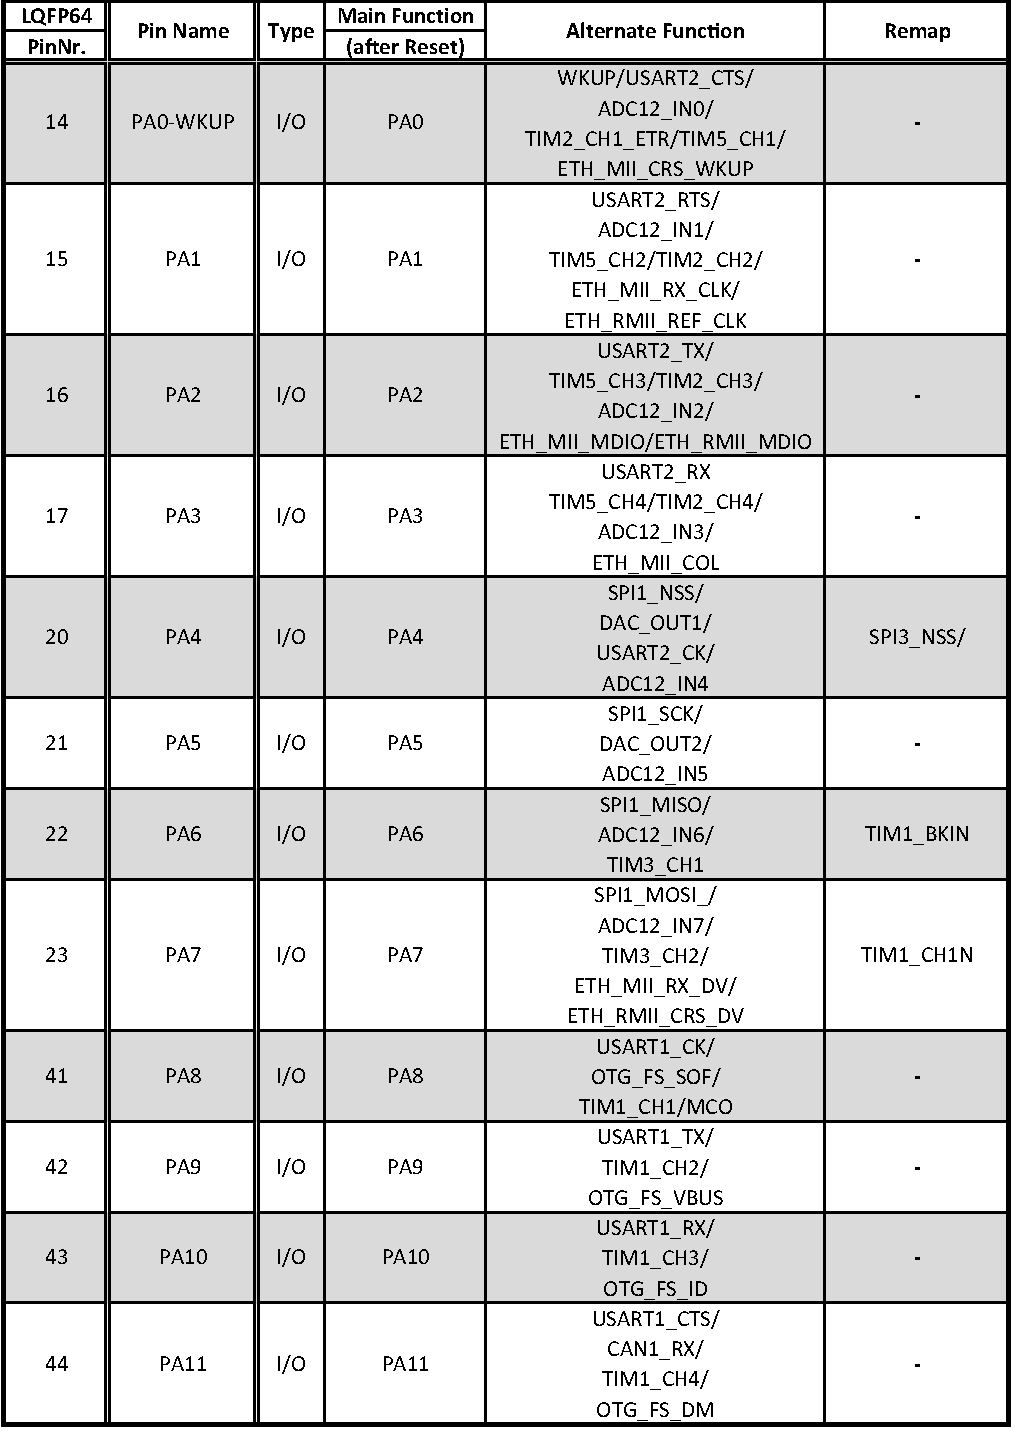
\includegraphics[width=0.8\textwidth]{Schuh/Pictures/Pinbelegung1}
    \caption[Pinbelegung des Prozessors]{Pinbelegung des Prozessors \cite{stm:stm32f107rc}}
    \label{tab:coremodul-cpupins}
\end{table}
\begin{table}[htb]\ContinuedFloat
    \centering
    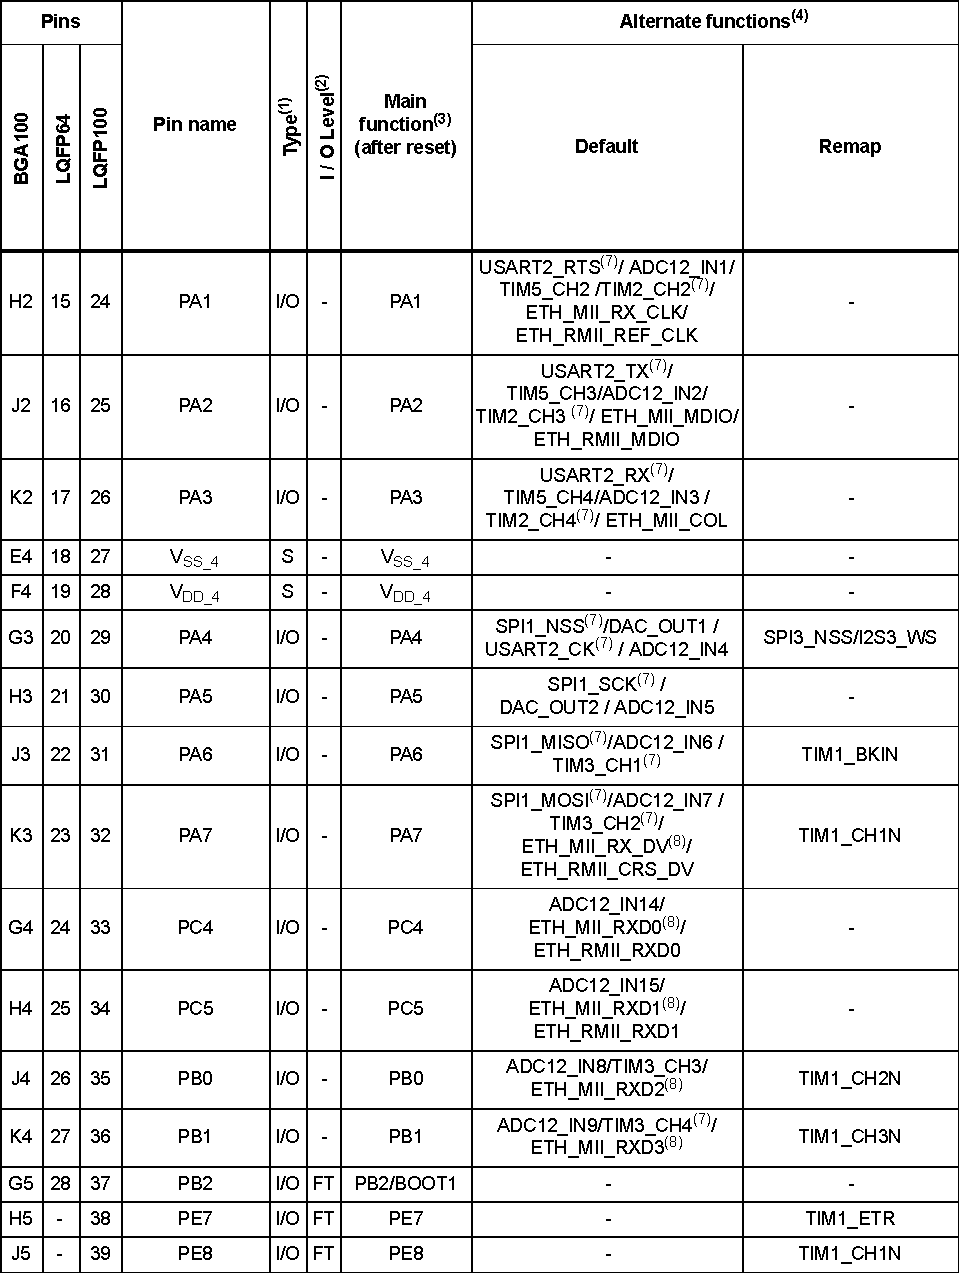
\includegraphics[width=0.8\textwidth]{Schuh/Pictures/Pinbelegung2}
    \caption[Pinbelegung des Prozessors]{Pinbelegung des Prozessors \cite{stm:stm32f107rc}}
\end{table}
\begin{table}[htb]\ContinuedFloat
    \centering
    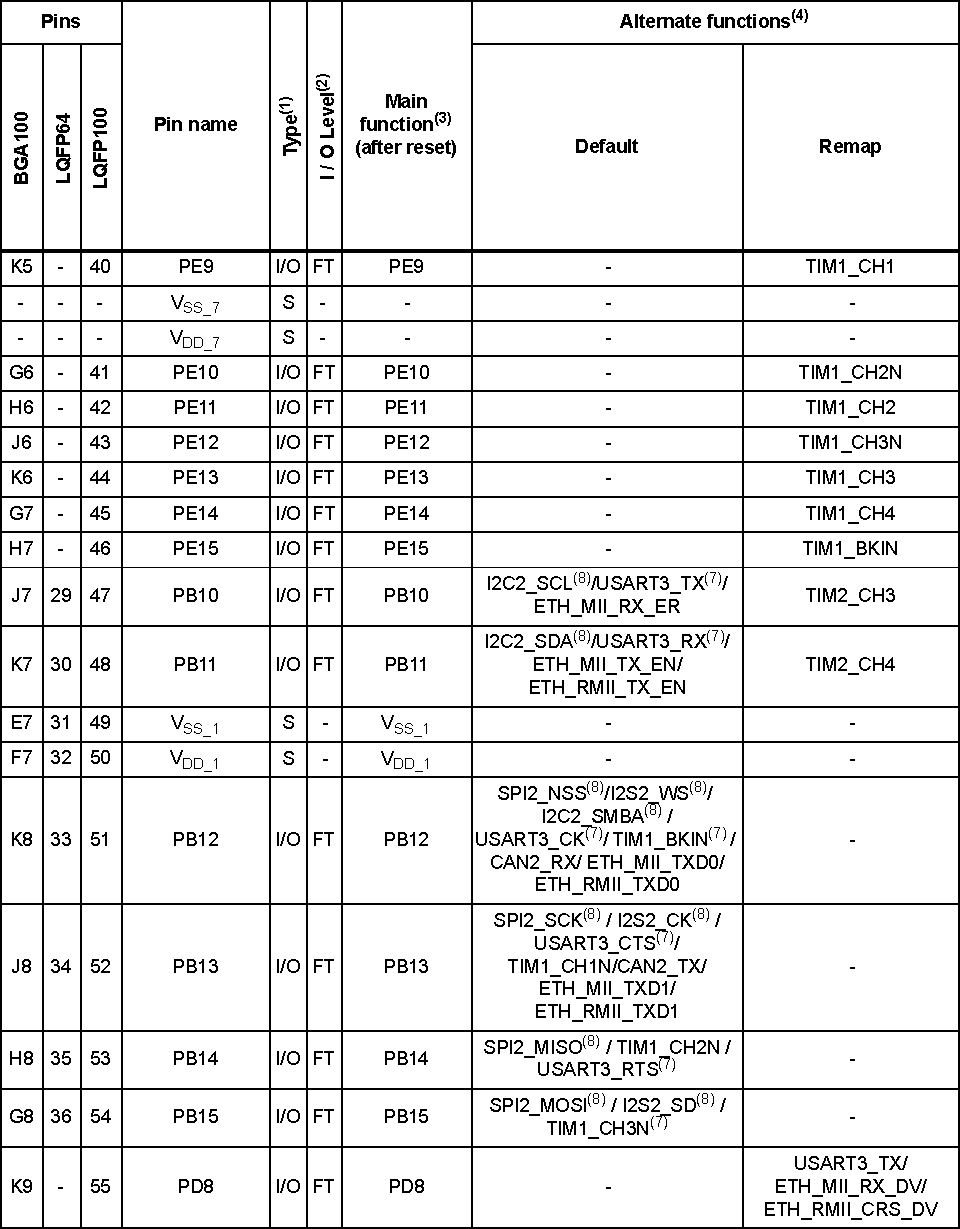
\includegraphics[width=0.8\textwidth]{Schuh/Pictures/Pinbelegung3}
    \caption[Pinbelegung des Prozessors]{Pinbelegung des Prozessors \cite{stm:stm32f107rc}}
\end{table}
\begin{table}[htb]\ContinuedFloat
    \centering
    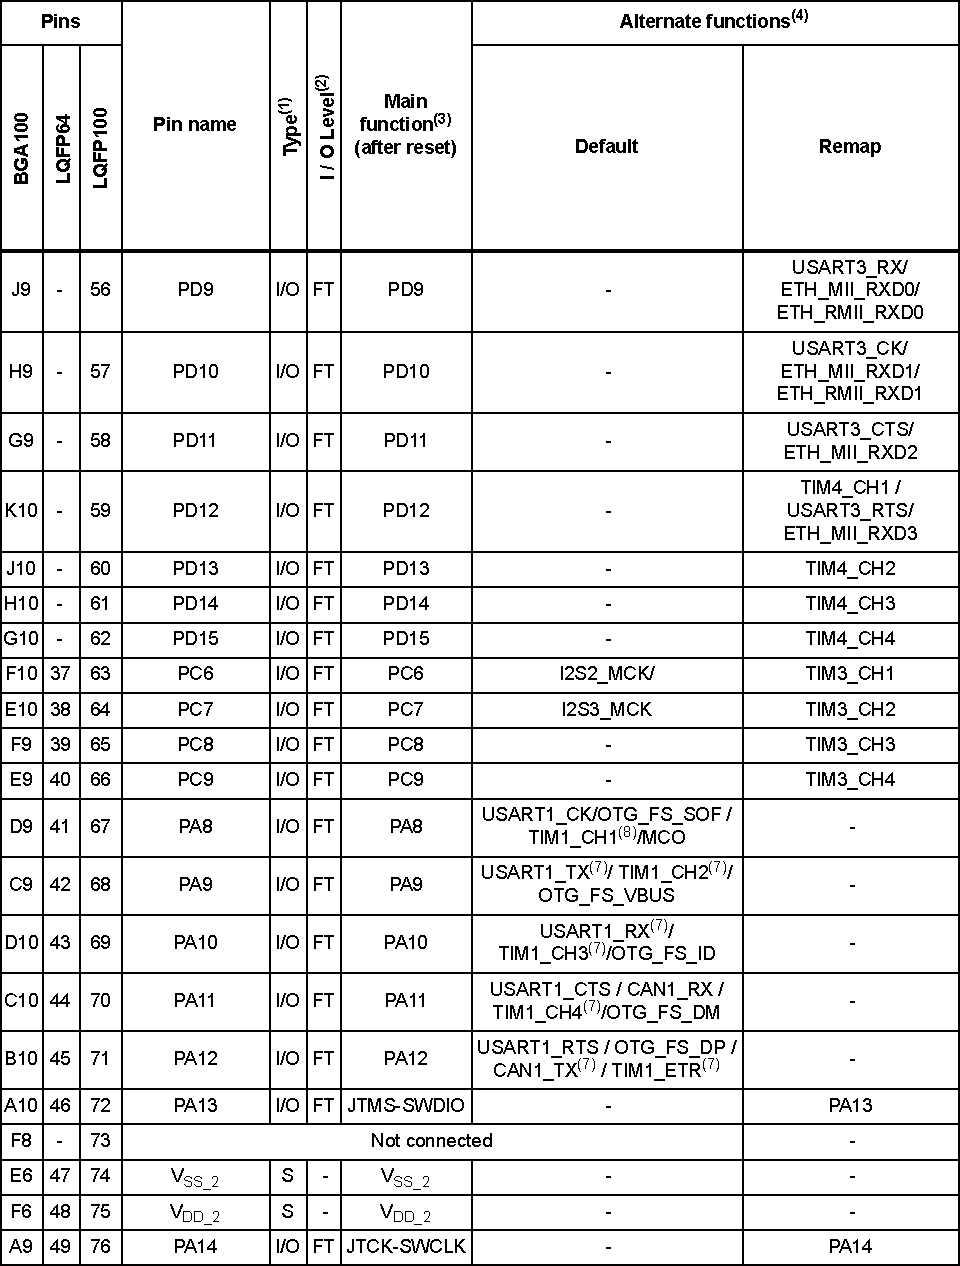
\includegraphics[width=0.8\textwidth]{Schuh/Pictures/Pinbelegung4}
    \caption[Pinbelegung des Prozessors]{Pinbelegung des Prozessors \cite{stm:stm32f107rc}}
\end{table}
\begin{table}[htb]\ContinuedFloat
    \centering
    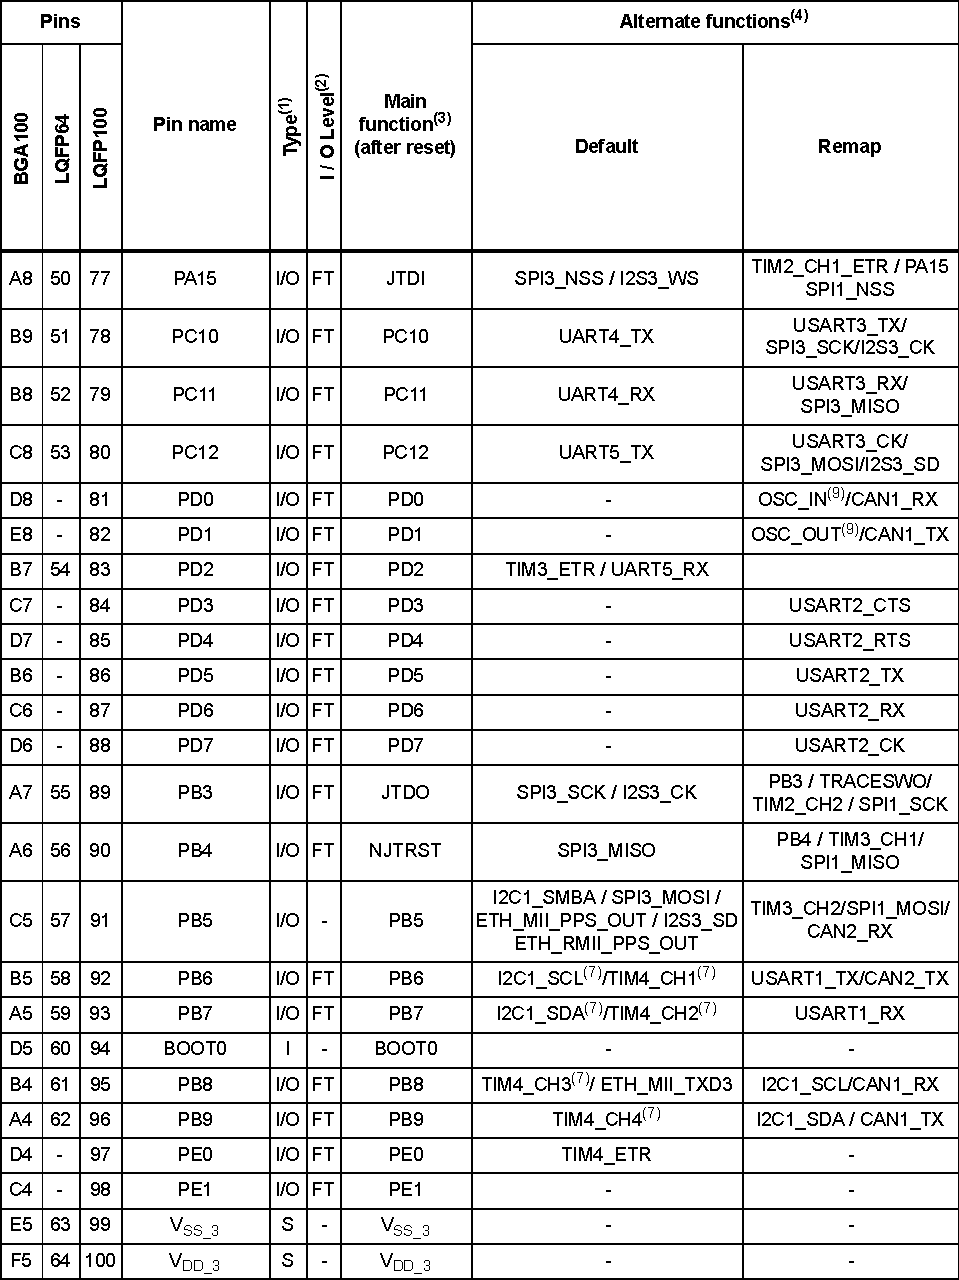
\includegraphics[width=0.8\textwidth]{Schuh/Pictures/Pinbelegung5}
    \caption[Pinbelegung des Prozessors]{Pinbelegung des Prozessors \cite{stm:stm32f107rc}}
\end{table}

\subsection{Portbelegungsplan}
\label{sec:coremodul-portbelegung}
\tabpdf{coremodul-portbelegung}{Portbelegungsplan des Core-Moduls}{Portbelegungsplan des \gls{Core-Modul}s}{0.5\textwidth}{Schuh/Pictures/Portbelegung}

\subsection{Gesamtschaltung}
\label{sec:coremodul-schaltung}
\fig{coremodul-gesamtschaltung}{Gesamtschaltung des Core-Moduls}{Gesamtschaltung des \gls{Core-Modul}s}{0.8\textwidth}{Schuh/Pictures/SchaltungCM}

\subsubsection{Programmierung mit ST-Link V2}
\label{sec:coremodul-stlink}
Zur Programmierung und zum \gls{Debugging} des neuen \gls{ARM}-\gls{Minimalsystem}s sollte ein \textbf{ST-Link V2 Mini} (\fref{fig:coremodul-stlink}) verwendet werden. Dieser Programmer besitzt eine verpolungssichere zweireihige Stiftreihe, welche es ermöglicht Programme mit Hilfe von \gls{SWD} auf den Microcontroller zu übertragen oder diese zu debuggen. Darüber hinaus ist der ST-Link V2 Mini der Lieferant der Hauptversorgungsspannung von \unit{+5}{\volt}.

Um den ST-Link V2 Mini und den Microcontroller im Falle eines Kurzschlusses zwischen der Versorgungsspannung und Masse zu schützen wurde eine Schottky-Diode (\fref{fig:coremodul-swd}, V1), mit einem maximalen Durchflussstrom von \unit{1}{\ampere}, vorgesehen. Um die Verpolungssicherheit des ST-Link V2 Mini zu gewährleisten, wurde eine zweireihige Buchsenleiste mit Nase (\fref{fig:coremodul-swd}, X1; \fref{fig:coremodul-stlinkbuchse}) verbaut, welche eine Verpolung des ST-Links unmöglich macht.

\fig{coremodul-stlink}{ST-Link V2 Mini}{ST-Link V2 Mini}{0.5\textwidth}{Schuh/Pictures/STLink}

\begin{figure}[htb]
    \centering
    \subfloat[Schematic\label{fig:coremodul-swd-schem}]{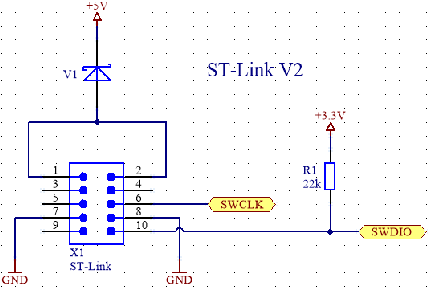
\includegraphics[width=.4\linewidth]{Schuh/Pictures/SchaltungSWD}}\qquad
\subfloat[Hardware\label{fig:coremodul-swd-hard}]{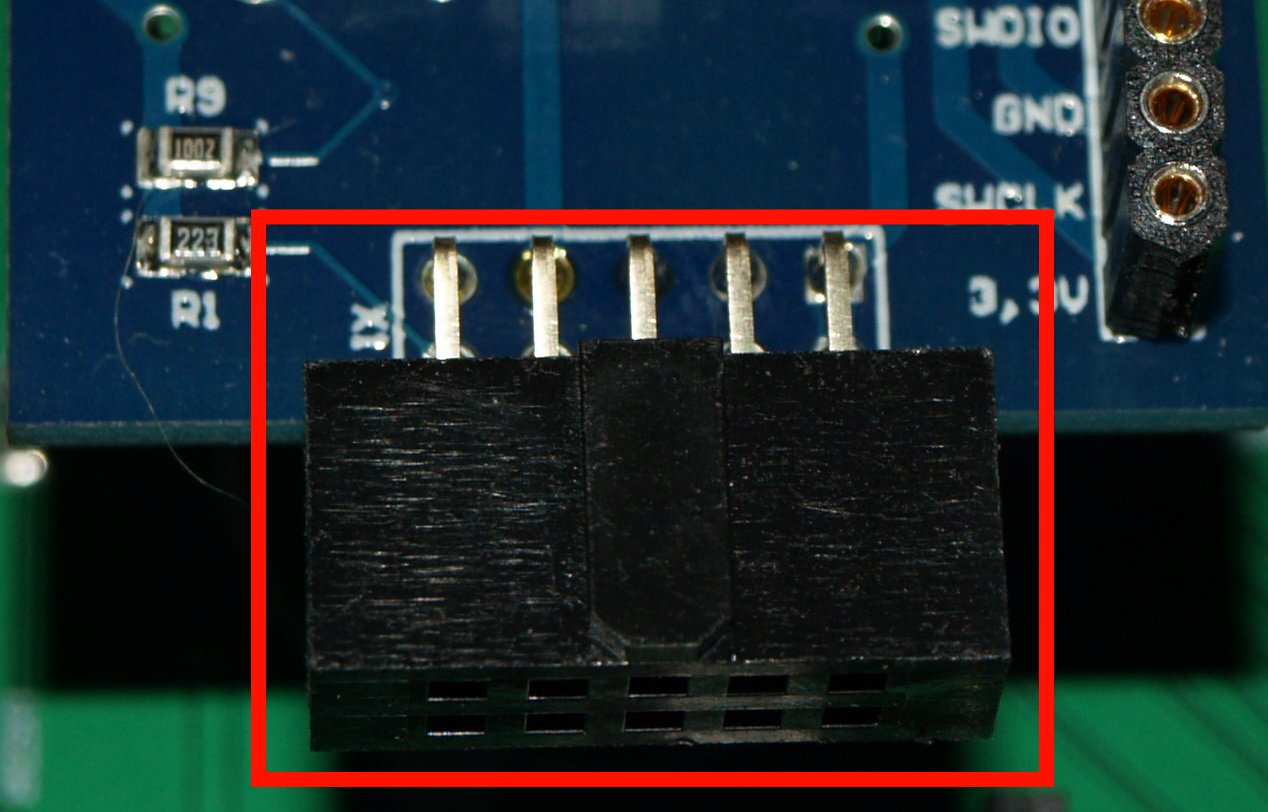
\includegraphics[width=.4\linewidth,angle=270]{Schuh/Pictures/core-stlink}}\qquad
    \caption[ST-Link Schaltung des Core-Moduls]{ST-Link Schaltung des \gls{Core-Modul}s}
    \label{fig:coremodul-swd}
\end{figure}

\fig{coremodul-stlinkbuchse}{Buchse mit Nase}{Buchse mit Nase}{0.5\textwidth}{Schuh/Pictures/STLinkBuchse}

\subsubsection{SWD-Adapter}
Der als Buchsenleiste ausgeführte SWD-Adapter (\fref{fig:coremodul-swd2}, X4), erfüllt vom Prinzip her die gleiche Funktion wie der bereits in \fref{sec:coremodul-stlink} beschriebene Stecker für den ST-Link V2 Mini. Dieser ermöglicht lediglich Kompatibilität zu anderen SWD-Programmern und Debuggern, welche diesen Stecker nicht besitzen.

\begin{figure}[htb]
    \centering
    \subfloat[Schematic\label{fig:coremodul-swd2-schem}]{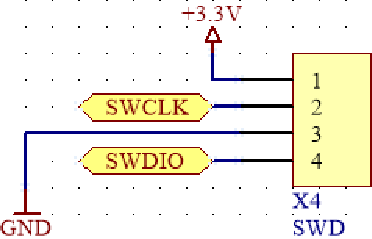
\includegraphics[width=.4\linewidth]{Schuh/Pictures/SchaltungSWD2}}\qquad
    \subfloat[Hardware\label{fig:coremodul-swd2-hard}]{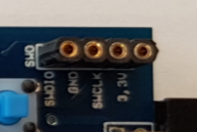
\includegraphics[width=.4\linewidth]{Schuh/Pictures/core-swd}}\qquad
    \caption[SWD-Schaltung des Core-Moduls]{SWD-Schaltung des \gls{Core-Modul}s}
    \label{fig:coremodul-swd2}
\end{figure}

\subsubsection{USART 1}
Die Buchsenleiste (\fref{fig:coremodul-uart}, X3) dient hauptsächlich zur seriellen Kommunikation. Die Pinanordnung wurde so gewählt, dass die Kommunikation entweder kabelgebunden, über den \gls{USB-to-UART} Adapter, oder alternativ über ein HC-06 Bluetooth Modul erfolgen kann.

\begin{figure}[htb]
    \centering
    \subfloat[Schematic\label{fig:coremodul-uart-schem}]{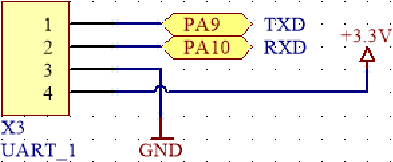
\includegraphics[width=.4\linewidth]{Schuh/Pictures/SchaltungUART}}\qquad
    \subfloat[Hardware\label{fig:coremodul-uart-hard}]{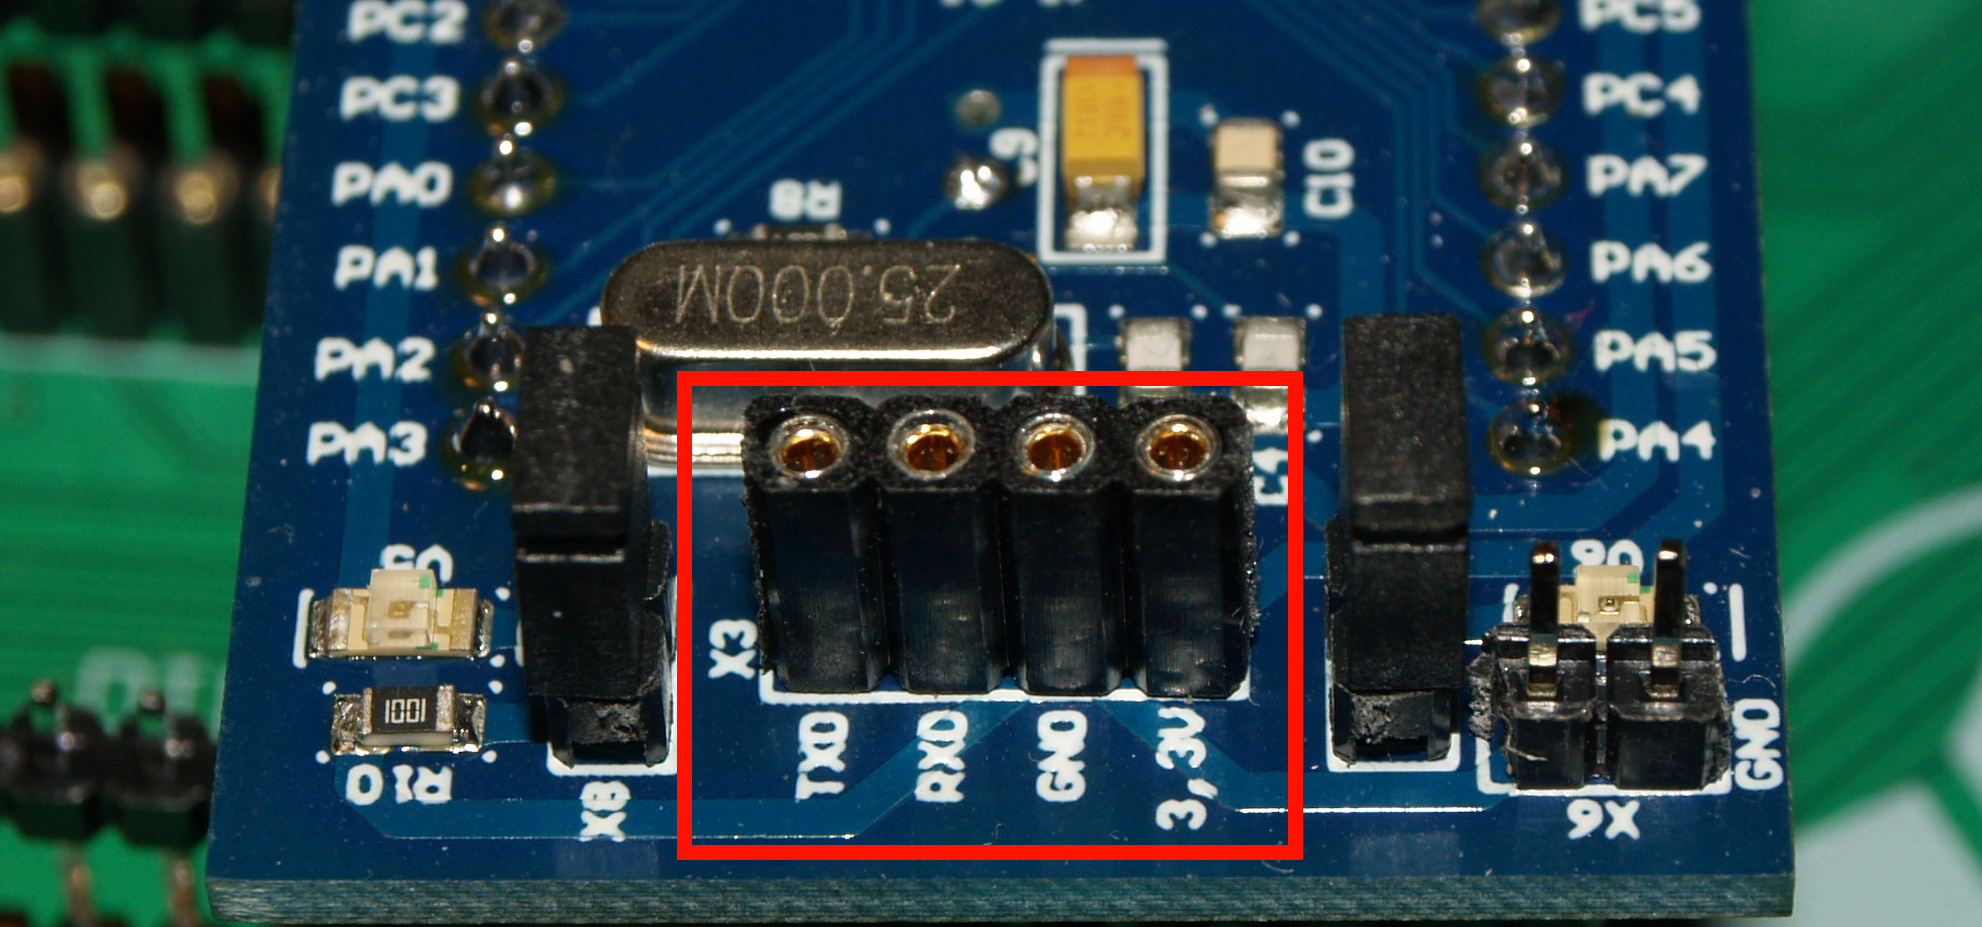
\includegraphics[angle=90,width=.4\linewidth]{Schuh/Pictures/core-uart}}\qquad
    \caption[UART-Schaltung des Core-Moduls]{UART-Schaltung des \gls{Core-Modul}s}
    \label{fig:coremodul-uart}
\end{figure}

\subsubsection{Bootkonfiguration}
Mit Hilfe des zweireihigen Bootjumpers (\fref{fig:coremodul-boot}, X5) kann der Benutzter entscheiden von welchem Speichermedium der Cortex booten soll.

Die Standardkonfiguration sieht vor, dass man vom Flash-Speicher bootet. Daher muss, wie in \fref{tab:coremodul-boot} beschrieben, Boot 0 auf GND gesetzt werden und Boot 1 auf +3.3V.

\fig{coremodul-boot}{Boot-Schaltung des Core-Moduls}{Boot-Schaltung des \gls{Core-Modul}s}{0.5\textwidth}{Schuh/Pictures/SchaltungBoot}
\tab{coremodul-boot}{Bootkonfigurationen des Core-Moduls}{Bootkonfigurationen des \gls{Core-Modul}s}{|c|c|p{10cm}|}{
    \hline
    \textbf{Boot 0} & \textbf{Boot 1} & \textbf{Funktion}\\
    \hline
    \unit{+3,3}{\volt} & \unit{+3,3}{\volt} & Booten von SRAM\\
    \hline
    \unit{+3,3}{\volt} & GND & Booten von Systemspeicher\\
    \hline
    GND & x & Booten von Flash-Speicher\\
    \hline
}

\subsubsection{Reset}
Der Kurzhubtaster (\fref{fig:coremodul-reset}, S2) dient zum Reset des \gls{Core-Modul}s. Mit Hilfe dieses ist ein erneuter Programmstart möglich, da er den Pin des low-aktiven Reset gegen Masse zieht. Gegebenenfalls angeschlossene Arduino-Shields werden mit diesem Taster ebenfalls zurückgesetzt.

\begin{figure}[htb]
    \centering
    \subfloat[Schematic\label{fig:coremodul-reset-schem}]{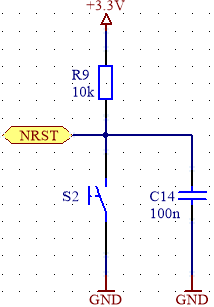
\includegraphics[width=.4\linewidth]{Schuh/Pictures/schaltung-reset}}\qquad
    \subfloat[Hardware\label{fig:coremodul-reset-hard}]{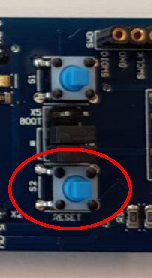
\includegraphics[width=.4\linewidth]{Schuh/Pictures/core-reset}}\qquad
    \caption[Reset-Schaltung des Core-Moduls]{Reset-Schaltung des \gls{Core-Modul}s}
    \label{fig:coremodul-reset}
\end{figure}

\subsubsection{\unit{5}{\volt} Spannungsversorgung}
Die \unit{+5}{\volt} Spannungsversorgung für das \gls{Core-Modul} kann auf zwei verschiedenen Wegen bezogen werden. Entweder man verwendet den ST-Link V2 Mini als \unit{5}{\volt} Spannungsversorgung (\fref{fig:coremodul-swd}, X1), wie bereits in \fref{sec:coremodul-stlink} beschrieben, oder man speist die \unit{+5}{\volt} Versorgung über den \unit{5}{\volt}-Pin am DIL-Adapter (\fref{fig:coremodul-spannung}, X2) ein.

\fig{coremodul-spannung}{Spannungsversorgungsschaltung des Core-Moduls}{Spannungsversorgungsschaltung des \gls{Core-Modul}s}{0.5\textwidth}{Schuh/Pictures/schaltung-spannung}

\subsubsection{Batterieversorgung}
An VB kann eine \unit{3,3}{\volt}-Batterie angeschlossen werden, damit die \gls{RTC} auch dann mit Spannung versorgt ist, wenn der Cortex-M3 außer Betrieb ist. Darüber hinaus wird im Falle des stromsparenden Deep-Sleep-Mode des Cortex-M3 ebenfalls eine Puffer-Batterie benötigt. Die Schottky-Diode (\fref{fig:coremodul-batterie}, V4) soll verhindern, dass die Batterie welche die \gls{RTC} des Cortex betreiben soll, nicht geladen wird. In den meisten Fällen handelt es sich bei dieser Batterie um eine Knopfzelle, welche häufig nicht wiederaufladbar ist. Die Schottky-Diode (\fref{fig:coremodul-batterie}, V3) soll verhindern, dass die Batteriespannung der \unit{3,3}{\volt}-Knopfzelle, mit der über einen Linearregler generierten Versorgungsspannung des Prozessors verbunden wird.

\fig{coremodul-batterie}{Batterieversorgungsschaltung des Core-Moduls}{Batterieversorgungsschaltung des \gls{Core-Modul}s}{0.5\textwidth}{Schuh/Pictures/schaltung-batterie}

\subsubsection{\unit{3,3}{\volt} Fixspannungsregler}
Zur Generierung der für den Prozessor erforderlichen Betriebsspannung wurde ein \unit{3,3}{\volt}-Linearregler (\fref{fig:coremodul-fix}, U2) verwendet, welcher die Eingangsspannung von \unit{+5}{\volt} auf \unit{+3,3}{\volt} herabsetzt. Bei Verwendung eines Linearreglers ist zu beachten, dass dieser die Spannungsdifferenz zwischen Ausgangsspannung und Eingangsspannung in Wärme umwandelt. Daher sollten keine temperaturempfindlichen Bauteile in dessen Nähe platziert werden. Zur Überprüfung ob das Modul mit der Betriebsspannung von \unit{+5}{\volt} versorgt wird, wurde die LED (\fref{fig:coremodul-fix}, V4) zur optischen Kontrolle eingebaut. Wenn das Modul mit Spannung versorgt wird, leuchtet diese. Zur Überprüfung ob der Prozessor mit seiner Betriebsspannung von \unit{3,3}{\volt} versorgt wird, wurde die LED (\fref{fig:coremodul-fix}, V6) zur optischen Kontrolle eingebaut. Wenn der Prozessor mit Spannung versorgt wird, leuchtet sie. Um den Stromverbrauch des \gls{Core-Modul}s im Low-Power Modus weiter zu senken, können die LEDs mit Hilfe von Jumpern außer Betrieb gesetzt werden.

\begin{figure}[htb]
    \centering
    \subfloat[Schematic\label{fig:coremodul-fix-schem}]{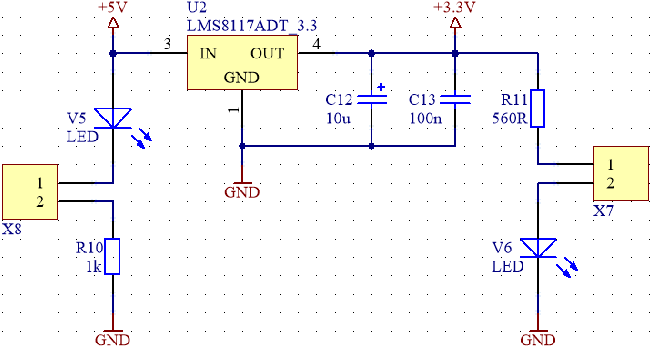
\includegraphics[width=.75\linewidth]{Schuh/Pictures/schaltung-fix}}\qquad
    \subfloat[Hardware\label{fig:coremodul-fix-hard}]{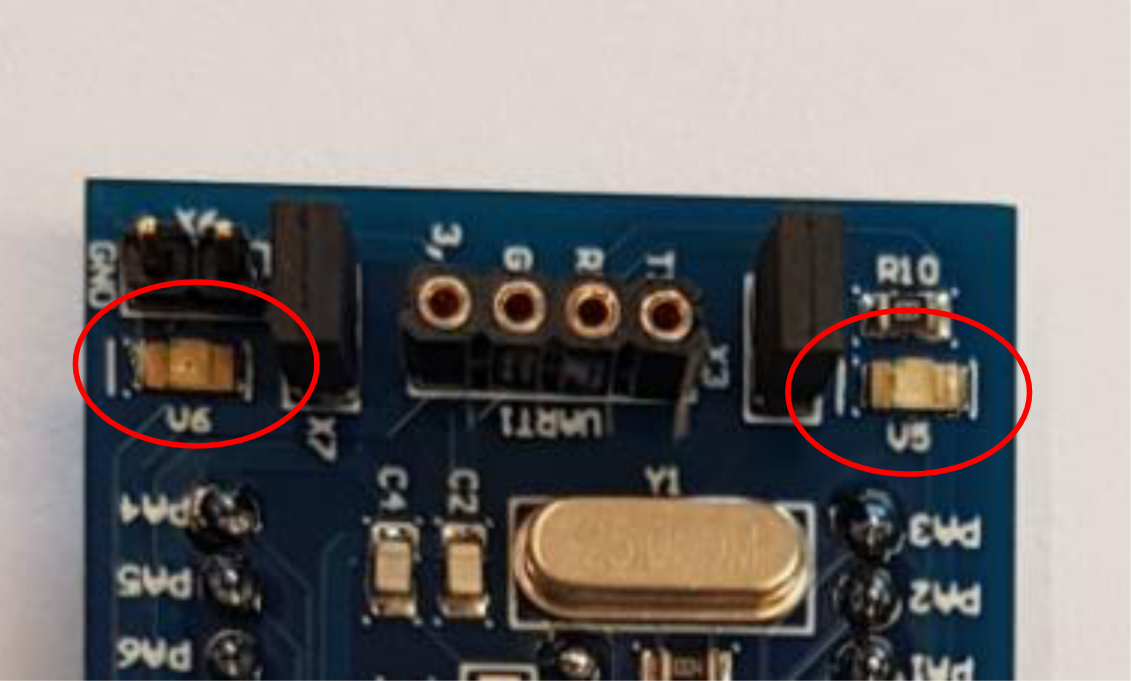
\includegraphics[width=.4\linewidth]{Schuh/Pictures/core-fix}}\qquad
    \caption[Fixspannungsregler des Core-Moduls]{Fixspannungsregler des \gls{Core-Modul}s}
    \label{fig:coremodul-fix}
\end{figure}


\subsubsection{Prozessor}
Das Schaltplansymbol für den Prozessor (\fref{fig:coremodul-prozessor}, U1) zeigt den im Schematic verwendeten Bauteil. Alle wichtigen Detailinformationen über den Prozessor wurden bereits in \fref{sec:coremodul-prozessor} behandelt.

\begin{figure}[htb]
    \centering
    \subfloat[Schematic\label{fig:coremodul-prozessor-schem}]{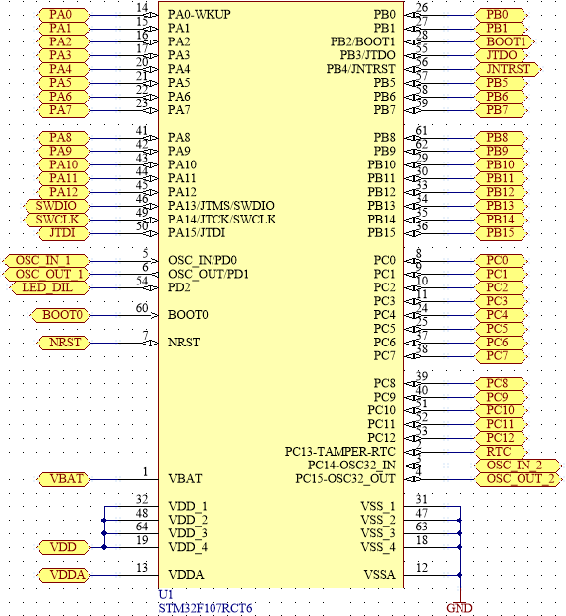
\includegraphics[width=.75\linewidth]{Schuh/Pictures/schaltung-prozessor}}\qquad
    \subfloat[Hardware\label{fig:coremodul-prozessor-hard}]{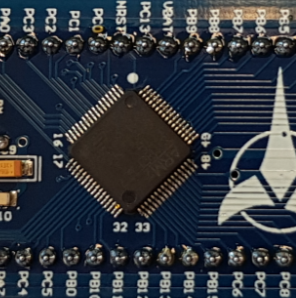
\includegraphics[width=.4\linewidth]{Schuh/Pictures/core-prozessor}}\qquad
    \caption[Prozessor des Core-Moduls]{Prozessor des \gls{Core-Modul}s}
    \label{fig:coremodul-prozessor}
\end{figure}

\subsubsection{Stützkondensatoren}
Während des laufenden Betriebs eines Microcontrollers benötigt dieser unterschiedlich viel Strom. Um auf diese Stromspitzen reagieren zu können, wurden Stützkondensatoren vorgesehen, damit es nicht zu Absturz des Programmes oder zu anderen Problemen durch Spannungseinbrüche kommt. Die Stützkondensatoren (\fref{fig:coremodul-kond}: C5, C6, C7 und C8) können daher die in ihnen gespeicherte Ladung bei stark wechselnden Stromaufnahmen abgeben und dadurch eine ordnungsmäßige Versorgung des Prozessors gewährleisten.

\fig{coremodul-kond}{Stützkondensatoren des Core-Moduls}{Stützkondensatoren des \gls{Core-Modul}s}{0.5\textwidth}{Schuh/Pictures/schaltung-kond}

\subsubsection{DIL-Adapter}
Das Schaltplansymbol des DIL-Adapters (\fref{fig:coremodul-dil}, X2) zeigt das Pinning, welches hardwaremäßig auf den zwei getrennten Buchsenleisten auf der Leiterkarte ausgeführt wurde.

\fig{coremodul-dil}{DIL-Adapter des Core-Moduls}{DIL-Adapter des \gls{Core-Modul}s}{0.5\textwidth}{Schuh/Pictures/schaltung-dil}

\subsubsection{Schwingquarze}
Das \gls{Core-Modul} besitzt standardmäßig zwei verschiedene Taktquellen. Diese bestehen aus einem 25MHz Quarz (\fref{fig:coremodul-quarz}, Y1), welcher für die Taktfrequenz des Prozessors zuständig ist, und einem 32kHz Quarz (\fref{fig:coremodul-quarz}, Y2), welcher für die interne \gls{RTC} zur Verfügung steht.

\fig{coremodul-quarz}{Schwingquarze des Core-Moduls}{Schwingquarze des \gls{Core-Modul}s}{0.75\textwidth}{Schuh/Pictures/schaltung-quarz}

\subsubsection{Taster}
Auf dem \gls{Core-Modul} wurde ein Kurzhubtaster (\fref{fig:coremodul-taster}, S1) vorgesehen, dessen Funktion nach belieben ausprogrammiert werden kann.

\begin{figure}[htb]
    \centering
    \subfloat[Schematic\label{fig:coremodul-taster-schem}]{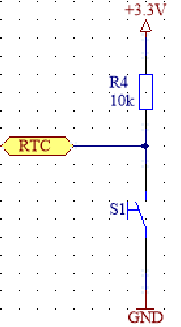
\includegraphics[width=.25\linewidth]{Schuh/Pictures/schaltung-taster}}\qquad
    \subfloat[Hardware\label{fig:coremodul-taster-hard}]{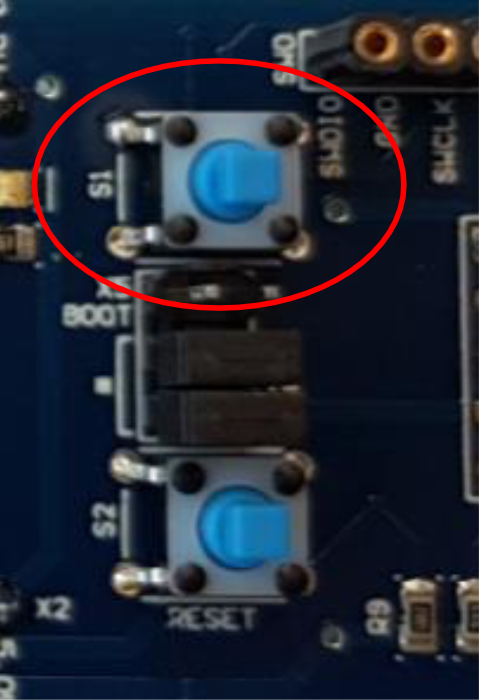
\includegraphics[width=.25\linewidth]{Schuh/Pictures/core-taster}}\qquad
    \caption[Taster des Core-Moduls]{Taster des \gls{Core-Modul}s}
    \label{fig:coremodul-taster}
\end{figure}

\subsubsection{LED}
Auf dem \gls{Core-Modul} wurde eine LED (\fref{fig:coremodul-led}, V2) vorgesehen, deren Funktion nach belieben ausprogrammiert werden kann.

\begin{figure}[htb]
    \centering
    \subfloat[Schematic\label{fig:coremodul-led-schem}]{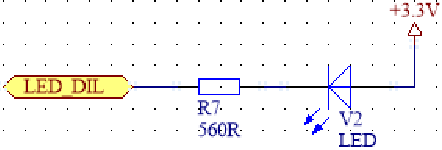
\includegraphics[width=.4\linewidth]{Schuh/Pictures/schaltung-led}}\qquad
    \subfloat[Hardware\label{fig:coremodul-led-hard}]{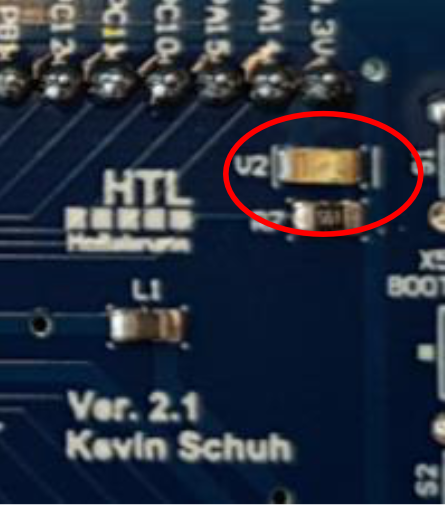
\includegraphics[width=.25\linewidth]{Schuh/Pictures/core-led}}\qquad
    \caption[LED des Core-Moduls]{LED des \gls{Core-Modul}s}
    \label{fig:coremodul-led}
\end{figure}

\subsubsection{Masseschleife}
Um das Messen mit einem Oszilloskop oder anderen Messgeräten zu vereinfachen wurde eine Masseschleife (\fref{fig:coremodul-masse}, X6) auf dem \gls{Core-Modul} realisiert.

\begin{figure}[htb]
    \centering
    \subfloat[Schematic\label{fig:coremodul-masse-schem}]{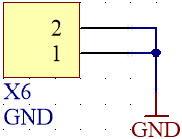
\includegraphics[width=.25\linewidth]{Schuh/Pictures/schaltung-masse}}\qquad
    \subfloat[Hardware\label{fig:coremodul-masse-hard}]{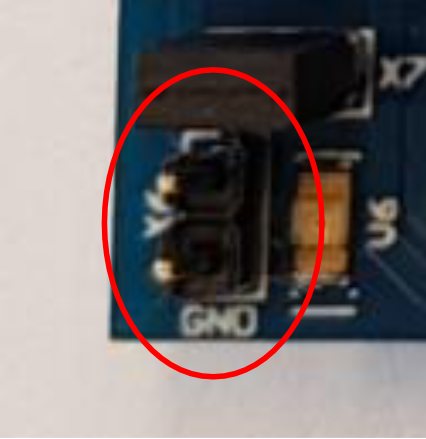
\includegraphics[width=.25\linewidth]{Schuh/Pictures/core-masse}}\qquad
    \caption[Masseschleife des Core-Moduls]{Masseschleife des \gls{Core-Modul}s}
    \label{fig:coremodul-masse}
\end{figure}

\subsection{Leiterplattenlayout}
\label{sec:coremodul-leiterplattenlayout}
\subsubsection{Bauteilseite}
\fig{coremodul-lbauteilseite}{Layout Bauteilseite des Core-Moduls}{Layout Bauteilseite des \gls{Core-Modul}s}{\textwidth}{Schuh/Pictures/core-lbauteilseite}

\subsubsection{Lötseite}
\fig{coremodul-llötseite}{Layout Lötseite des Core-Moduls}{Layout Lötseite des \gls{Core-Modul}s}{\textwidth}{Schuh/Pictures/core-llotseite}

\subsection{Bestückungspläne}
\label{sec:coremodul-bestückungspläne}
\subsubsection{Bauteilseite}
\fig{coremodul-bbauteilseite}{Bestückungsplan Bauteilseite des Core-Moduls}{Bestückungsplan Bauteilseite des \gls{Core-Modul}s}{\textwidth}{Schuh/Pictures/core-bbauteilseite}

\subsubsection{Lötseite}
\fig{coremodul-blötseite}{Bestückungsplan Lötseite des Core-Moduls}{Bestückungsplan Lötseite des \gls{Core-Modul}s}{\textwidth}{Schuh/Pictures/core-blotseite}
\section{Basisplatine}
\label{sec:basisplatine}

\fig{core-modul}{Basisplatine}{\gls{Basisplatine}}{\textwidth}{Schuh/Pictures/basis}

\subsection{Allgemeines}
\label{sec:basisplatine-allgemeines}
Die \gls{Basisplatine} dient dazu dem \gls{Core-Modul} eine umfangreiche, moderne und jederzeit erneuerbare Peripherie bereit zu stellen, um verschiedene Anwendungskonzepte schnell und einfach evaluieren zu können. Darüber hinaus soll mit Hilfe der \gls{Basisplatine} eine Versorgung und Programmierung des \gls{Core-Modul}s möglich sein. Durch Verwendung des Arduino-Shield-Konnektors können alle am Markt verfügbaren Arduino-Shields verwendet werden, daher kann man jederzeit Hardwarekomponenten tauschen oder selbst entwickeln.

\subsection{Schnittstellen}
\label{sec:basisplatine-schnittstellen}

Die \gls{Basisplatine} verfügt über mehrere in \fref{tab:basisplatine-schnittstellen} angegebene Schnittstellen. In \fref{fig:basisplatine-plan} dargestellt wie diese auf der \gls{Basisplatine} platziert sind.

\tab{basisplatine-schnittstellen}{Schnittstellen der Basisplatine}{Schnittstellen der \gls{Basisplatine}}{|c|p{10cm}|}{
    \hline
    \textbf{Schnittstelle} & \textbf{Funktion}\\
    \hline
    USART 1 & Ansteuerung von HC-06, HC-12, \gls{USB-to-UART}-Adapter, MAX232\\
    \hline
    USART 2 & Ansteuerung von ESP8266, XBee-Pro\\
    \hline
    USART 3 & Ansteuerung von Nextion-Display\\
    \hline
    SPI 1 & \\
    \hline
    \IIC{} 1 & \\
    \hline
    SWD & Programmierung auf Basis von \gls{SWD}\\
    \hline
    ST-Link V2 & Programmierung auf Basis von \gls{SWD}\\
    \hline
    JTAG & Programmierung auf Basis von \gls{JTAG}\\
    \hline
    DE-9 Buche & Ansteuerung von Nextion-Display\\
    \hline
    Arduino-Shield-Connector & Verwendung von diversen Arduino-Shields\\
    \hline
    Audio-Shield-Connector & Verwendung des HTL-internen Audio-Shields\\
    \hline
    Singe-Wire & Ansteuerung von Piezo, Temperatursensor, LFU, IR-Sensor, BMA020, EEPROM\\
    \hline
    USB-A & Spannungsversorgung, Datentransport\\
    \hline
    USB-B & Spannungsversorgung, Datentransport\\
    \hline
}

\fig{basisplatine-plan}{Übersichtsplan der Basisplatine}{Übersichtsplan der \gls{Basisplatine}}{\textwidth}{Schuh/Pictures/Basisplatine}

\subsection{Portbelegungsplan}
\label{sec:basisplatine-portbelegung}
\tabpdf{basisplatine-portbelegung}{Portbelegungsplan der Basisplatine}{Portbelegungsplan der \gls{Basisplatine}}{0.45\textwidth}{Schuh/Pictures/Basis-Portbelegung}

\subsubsection{ST-Link V2}
\label{sec:basisplatine-stlink}
Zur Programmierung und zum \gls{Debugging} des neuen \gls{ARM}-\gls{Minimalsystem}s sollte ein \textbf{ST-Link V2 Mini} verwendet werden. Dieser Programmer besitzt eine verpolungssichere zweireihige Stiftreihe, welche es ermöglicht Programme mit Hilfe von \gls{SWD} auf den Microcontroller zu übertragen oder diese zu debuggen. Darüber hinaus ist der ST-Link V2 Mini der Lieferant der Hauptversorgungsspannung von \unit{+5}{\volt}.

Um den ST-Link V2 Mini und den Microcontroller im Falle eines Kurzschlusses zwischen der Versorgungsspannung und Masse zu schützen wurde eine Schottky-Diode V16 (\fref{fig:basisplatine-swd}), mit einem maximalen Durchflussstrom von \unit{3}{\ampere}, vorgesehen.

\begin{figure}[H]
    \centering
    \subfloat[Schematic\label{fig:basisplatine-swd-schem}]{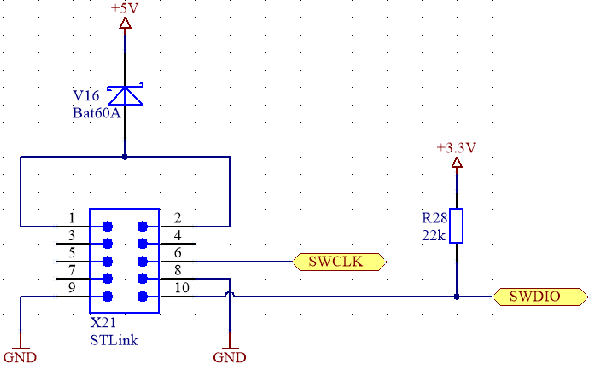
\includegraphics[width=.6\linewidth]{Schuh/Pictures/Basis-SWD}}\qquad
    \subfloat[Hardware\label{fig:basisplatine-swd-hard}]{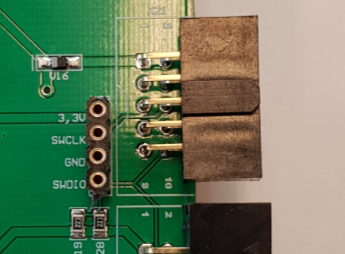
\includegraphics[width=.3\linewidth]{Schuh/Pictures/basis-stlink}}\qquad
    \caption[ST-Link Schaltung der Basisplatine]{ST-Link Schaltung der \gls{Basisplatine}}
    \label{fig:basisplatine-swd}
\end{figure}

\subsubsection{SWD-Adapter}
Der als Buchsenleiste ausgeführte SWD-Adapter X23 (\fref{fig:basisplatine-swd2}), erfüllt vom Prinzip her die gleiche Funktion wie der bereits in \fref{sec:basisplatine-stlink} beschriebene Stecker für den ST-Link V2 Mini. Dieser ermöglicht lediglich Kompatibilität zu anderen SWD-Programmern und Debuggern, welche diesen Stecker nicht besitzen.

\begin{figure}[H]
    \centering
    \subfloat[Schematic\label{fig:basisplatine-swd2-schem}]{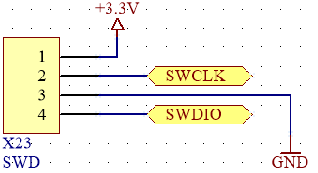
\includegraphics[width=.4\linewidth]{Schuh/Pictures/Basis-SWD2}}\qquad
    \subfloat[Hardware\label{fig:basisplatine-swd2-hard}]{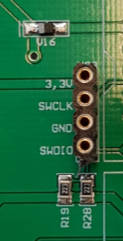
\includegraphics[width=.2\linewidth]{Schuh/Pictures/basis-swd}}\qquad
    \caption[SWD-Schaltung der Basisplatine]{SWD-Schaltung der \gls{Basisplatine}}
    \label{fig:basisplatine-swd2}
\end{figure}

\subsubsection{JTAG}
Zur Programmierung und zum \gls{Debugging} des neuen \gls{ARM}-\gls{Minimalsystem}s wurde aus kompatibilitätsgründen zum alten System zusätzlich vollwertige JTAG-Schnittstelle vorgesehen, um weiterhin mit Hilfe des ULINK/ME Adapters arbeiten zu können. Auch diese Schnittstelle besitzt eine verpolungssichere zweireihige Buchsenleiste X19 (\fref{fig:basisplatine-jtag}), welche es ermöglicht Programme mit Hilfe des JTAG-Protokolls auf den Microcontroller zu übertragen oder diese zu debuggen.

\begin{figure}[H]
    \centering
    \subfloat[Schematic\label{fig:basisplatine-jtag-schem}]{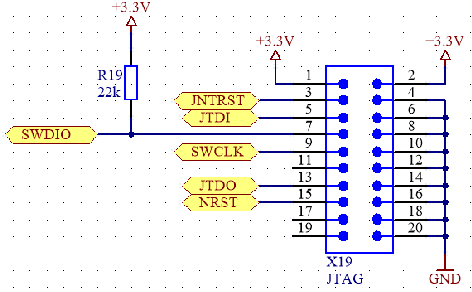
\includegraphics[width=.5\linewidth]{Schuh/Pictures/Basis-JTAG}}\qquad
    \subfloat[Hardware\label{fig:basisplatine-jtag-hard}]{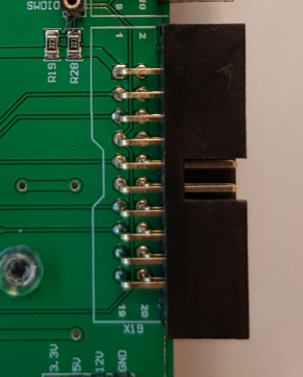
\includegraphics[width=.3\linewidth]{Schuh/Pictures/basis-jtag}}\qquad
    \caption[JTAG-Schaltung der Basisplatine]{JTAG-Schaltung der \gls{Basisplatine}}
    \label{fig:basisplatine-jtag}
\end{figure}

\subsubsection{Core-Modul-Adapter}
Das Schaltplansymbol des \gls{Core-Modul}s X20 (\fref{fig:basisplatine-core}) zeigt das Pinning, welches auf zwei Buchsenleisten auf der \gls{Basisplatine} herausgeführt wurde.

\begin{figure}[H]
    \centering
    \subfloat[Schematic\label{fig:basisplatine-core-schem}]{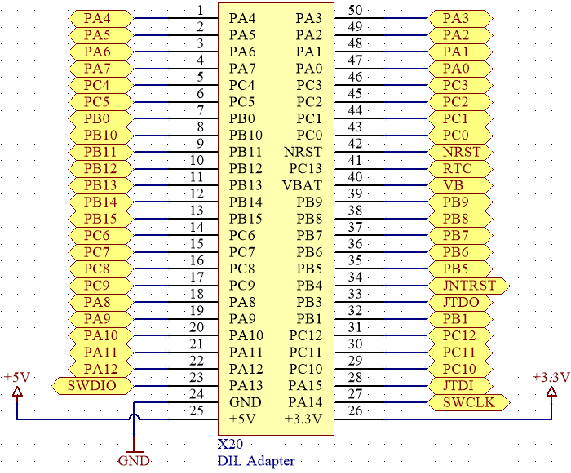
\includegraphics[width=.5\linewidth]{Schuh/Pictures/Basis-core}}\qquad
    \subfloat[Hardware\label{fig:basisplatine-core-hard}]{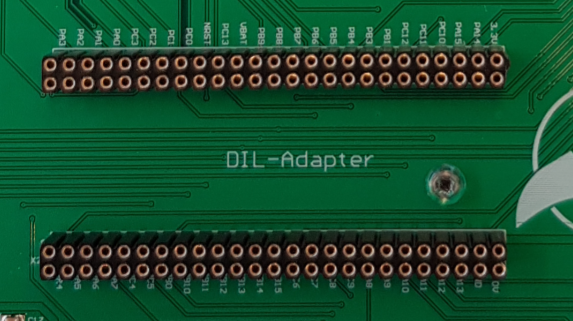
\includegraphics[width=.5\linewidth]{Schuh/Pictures/basis-core}}\qquad
    \caption[Core-Modul-Adapter der Basisplatine]{\gls{Core-Modul}-Adapter der \gls{Basisplatine}}
    \label{fig:basisplatine-core}
\end{figure}

\subsubsection{Audio-Adapter}
Der bereits in einer anderen Diplomarbeit realisierte Audio-Adapter kann auf der zweireihigen Buchsenleiste X24 (\fref{fig:basisplatine-audio}) aufgesteckt und anschließend betrieben werden.

\begin{figure}[H]
    \centering
    \subfloat[Schematic\label{fig:basisplatine-audio-schem}]{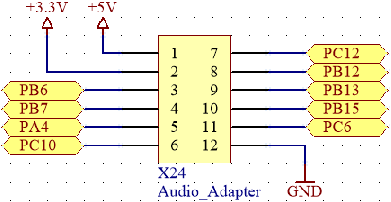
\includegraphics[width=.4\linewidth]{Schuh/Pictures/Basis-audio}}\qquad
    \subfloat[Hardware\label{fig:basisplatine-audio-hard}]{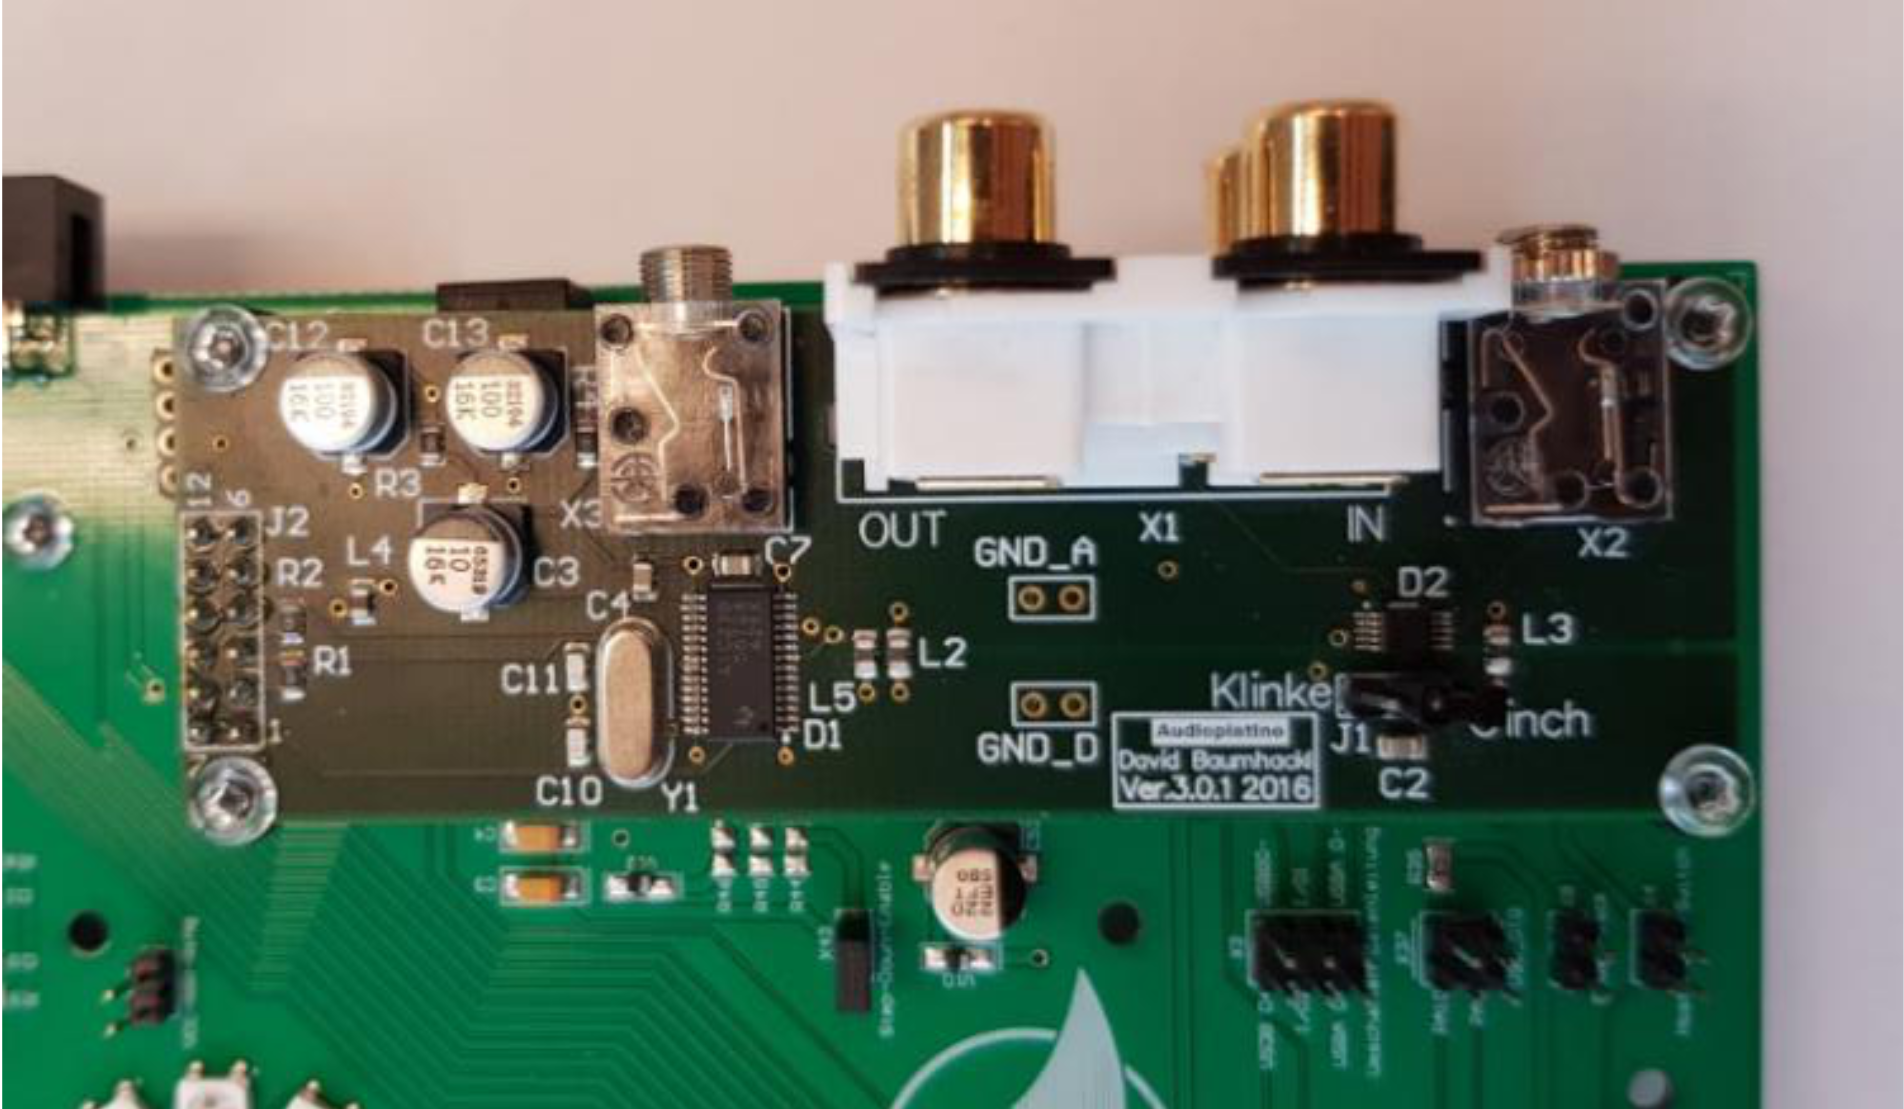
\includegraphics[width=.4\linewidth]{Schuh/Pictures/basis-audio}}\qquad
    \caption[Audio-Adapter der Basisplatine]{Audio-Adapter der \gls{Basisplatine}}
    \label{fig:basisplatine-audio}
\end{figure}

\subsubsection{LED-Array}
Auf der \gls{Basisplatine} wurde ein LED-Array realisiert, welches aus acht LEDs besteht und über die Portleitungen PC1 bis PC5 und PC7 bis PC8 (\fref{fig:basisplatine-leds}) angesteuert werden können. Diese LEDs sind in SMD-Form ausgeführt und haben die einheitliche Farbe Grün. Mit Hilfe der Stiftleiste X18 (\fref{fig:basisplatine-leds}) und deinem Jumper können die LEDs aktiviert oder deaktiviert werden. Wenn der Jumper entfernt ist sind die LEDs deaktiviert und die belegten Port-Pins des \gls{Core-Modul}s sind wieder frei verfügbar.

\begin{figure}[H]
    \centering
    \subfloat[Schematic\label{fig:basisplatine-leds-schem}]{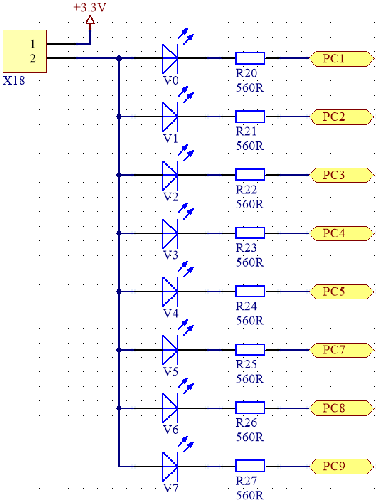
\includegraphics[width=.3\linewidth]{Schuh/Pictures/Basis-leds}}\qquad
    \subfloat[Hardware\label{fig:basisplatine-leds-hard}]{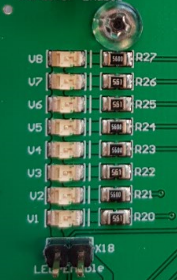
\includegraphics[width=.3\linewidth]{Schuh/Pictures/basis-leds}}\qquad
    \caption[LED-Array der Basisplatine]{LED-Array der \gls{Basisplatine}}
    \label{fig:basisplatine-leds}
\end{figure}

\subsubsection{DIP-Switches}
\label{sec:basis-dip}
Auf der \gls{Basisplatine} wurde ein achtpoliger DIP-Switch realisiert, welcher intern aus acht getrennten Schalten besteht und über die Portleitungen PA0 bis PA3 und PA5 bis PA8 (\fref{fig:basisplatine-dip}) ausgelesen werden kann. Da im Hardwarelayout keine Pullup-Widerstände vorgesehen wurden, muss bei der Programmierung darauf geachtet werden, dass die internen Pullup-Widerstände des Prozessors aktiviert sind. Da jedoch Port Pins PA2 und PA3 mit der UART2-Schnittstelle verbunden sind, erzeugen diese ein Echo, wenn die Schalter S3 und S4 gleichzeitig geschlossen sind. Weiters können durch Jumpern der Stiftleiste X22 (\fref{fig:basisplatine-dip}) alle Schalter im Kippschalter aktiviert oder deaktiviert werden.

\begin{figure}[H]
    \centering
    \subfloat[Schematic\label{fig:basisplatine-dip-schem}]{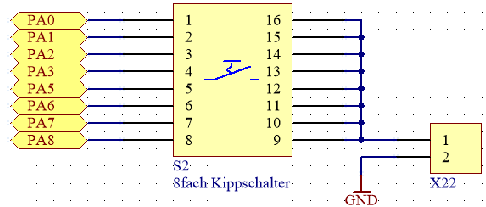
\includegraphics[width=.4\linewidth]{Schuh/Pictures/Basis-dip}}\qquad
    \subfloat[Hardware\label{fig:basisplatine-dip-hard}]{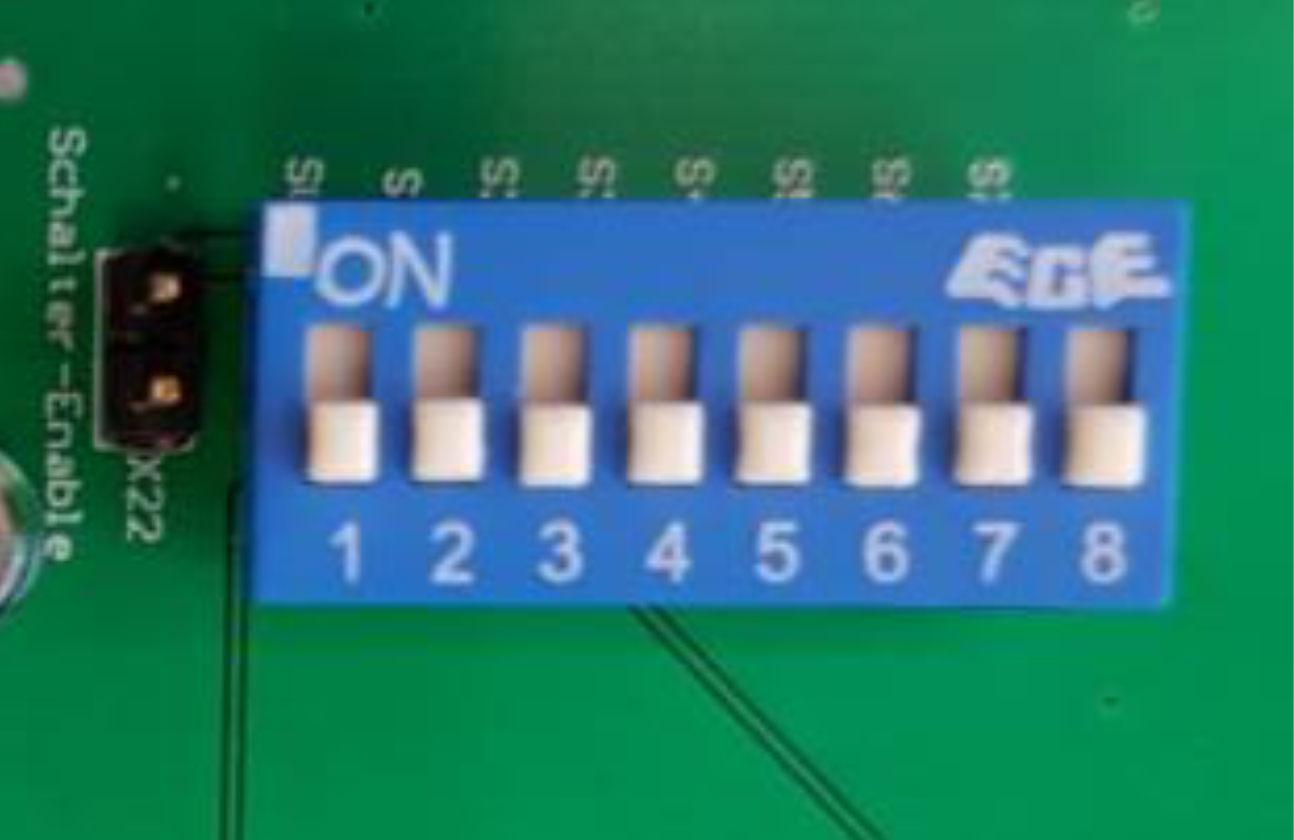
\includegraphics[width=.4\linewidth]{Schuh/Pictures/basis-dip}}\qquad
    \caption[DIP-Switches der Basisplatine]{DIP-Switches der \gls{Basisplatine}}
    \label{fig:basisplatine-dip}
\end{figure}

\subsubsection{USB-Varianten und Versorgung über USB}
Die \gls{Basisplatine} unterstützt hardwaremäßig zwei verschiedene USB-Bauformen und drei verschiedene USB-Funktionen. Diese USB-Funktionen sind USB-Device, USB-Host, USB-OTG (on the go) und werden sowohl von der USB-A Buchse X3 (\fref{fig:basisplatine-usb}), als auch von der USB-B Buchse X1 (\fref{fig:basisplatine-usb}) unterstützt. Da beide Buchsenformen keine ID-Leitung besitzen muss für USB-OTG die dafür benötigte Portleitung PA10 mit einem Pullup-Widerstand versehen werden, um den USB-OTG Modus vorzutäuschen. Weiters müssen für den USB-OTG Modus der Pin1 mit dem Pin2 und der Pin3 mit dem Pin4 auf der zweireihigen Stiftleiste X37 (\fref{fig:basisplatine-usb}) gejumpert werden. Über die Portleitung PA10 kann ausgewählt werden ob der Prozessor als USB-Host oder USB-Device arbeitet. Mit der Portleitung PA9 hingegen kann festgestellt werden ob die Versorgung über die USB Buchse funktioniert.

Falls man im Host-Modus Geräte ohne Adapter anschließen möchte, wurde eine zweite USB Buchse parallel geschaltet. Sollte man die USB-B Buchse auswählen wollen muss man den Pin1 mit dem Pin3 und dem Pin2 mit dem Pin4 auf der zweireihigen Stiftleiste X2 (\fref{fig:basisplatine-usb}) jumpern. Um die USB-A Buchse auswählen muss man den Pin4 mit dem Pin6 und dem Pin3 mit dem Pin5 auf der zweireihigen Stiftleiste X2 (\fref{fig:basisplatine-usb}) jumpern.

Die Feinsicherung F2 (\fref{fig:basisplatine-usb}) dient zur Absicherung des USB-Hosts, welcher die Versorgungsspannung normalerweise zur Verfügung stellt. Laut USB-Spezifikation ist hierbei bei USB 2.0 ein maximaler Strom von \unit{500}{\milli\ampere} erlaubt. Die Sicherung stellt sicher, dass dieser Strom niemals überschritten wird.

Die ESD Protection F1 (\fref{fig:basisplatine-usb}) stellt sicher, dass die Spannungen auf den Datenleitungen zwischen GND und \unit{5}{\volt} bleiben. Durch an- und abstecken an Host-Geräte können Spannungsspitzen auf den Datenleitungen auftreten, die ESD Protection leitet diese ab, sodass der Prozessor nicht beschädigt wird.

\begin{figure}[H]
    \centering
    \subfloat[Schematic\label{fig:basisplatine-usb-schem}]{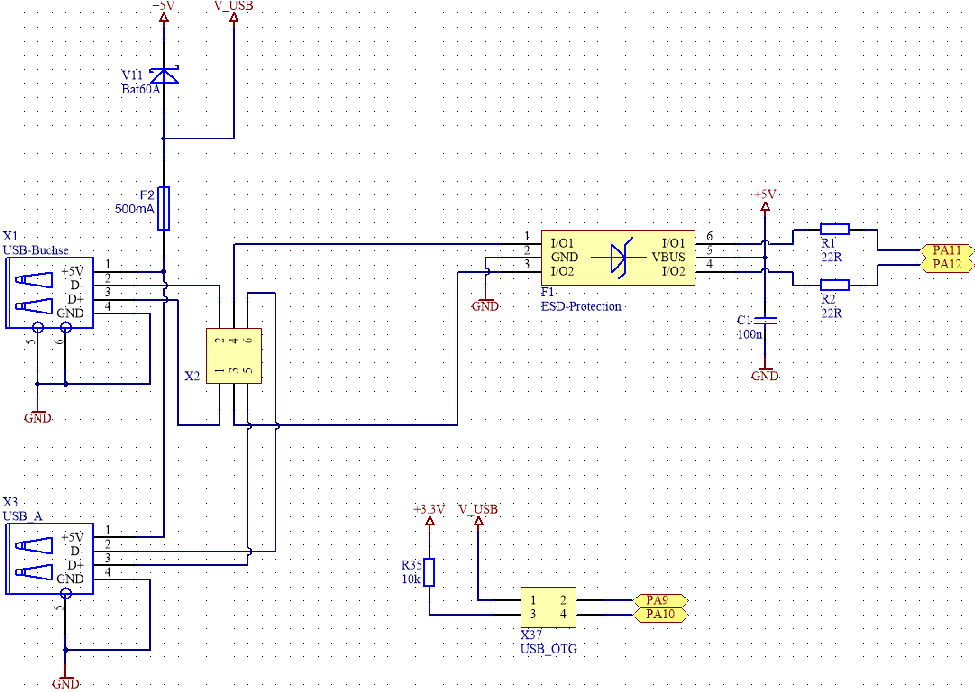
\includegraphics[width=\linewidth]{Schuh/Pictures/Basis-usb}}\qquad
    \subfloat[Hardware\label{fig:basisplatine-usb-hard}]{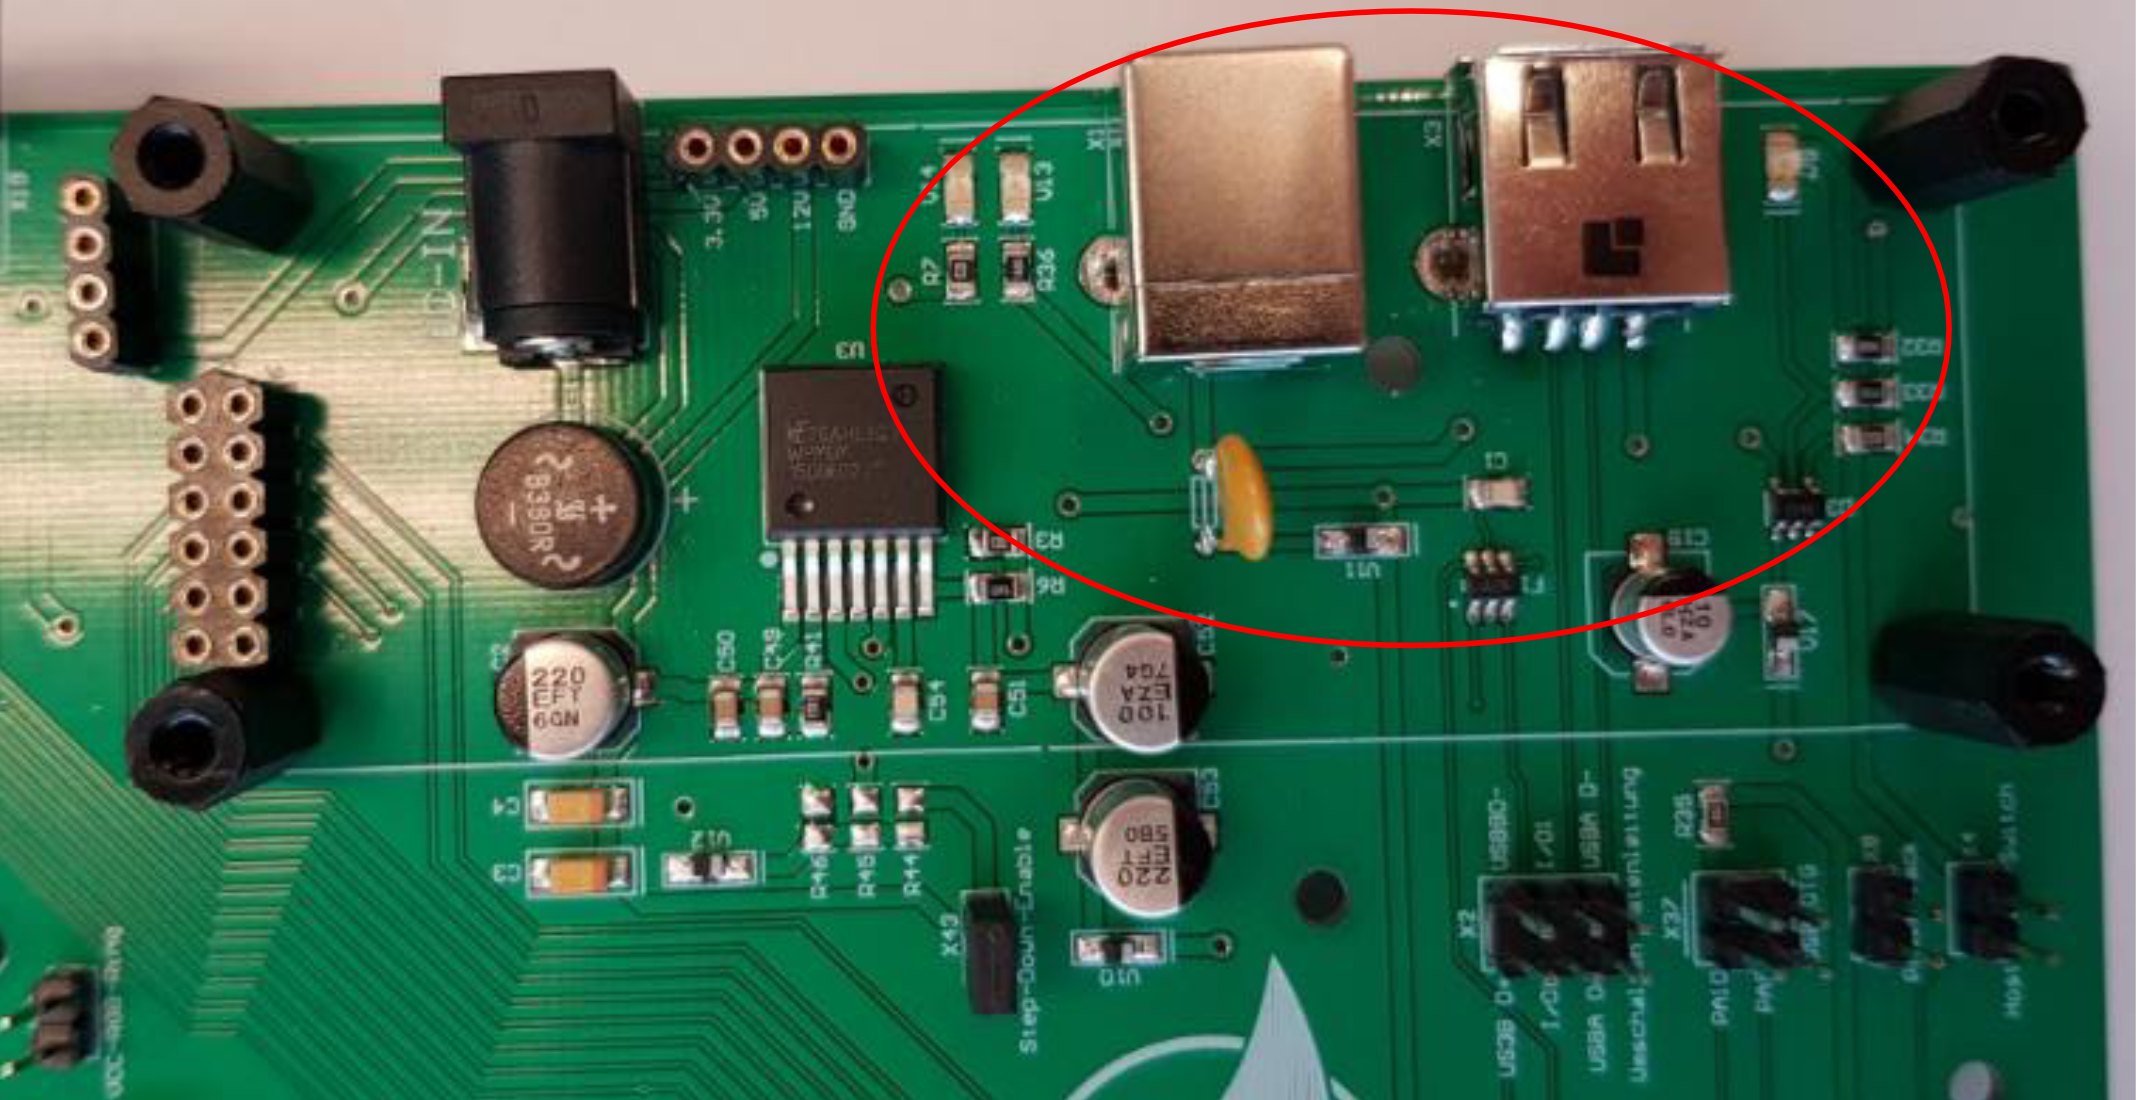
\includegraphics[width=\linewidth]{Schuh/Pictures/basis-usb}}\qquad
    \caption[USB Buchsen der Basisplatine]{USB Buchsen der \gls{Basisplatine}}
    \label{fig:basisplatine-usb}
\end{figure}

\subsubsection{Masseschleife}
Um das Messen mit einem Oszilloskop oder anderen Messgeräten zu vereinfachen wurde eine Masseschleife X5 (\fref{fig:basisplatine-masse}) auf der \gls{Basisplatine} realisiert.

\begin{figure}[H]
    \centering
    \subfloat[Schematic\label{fig:basisplatine-masse-schem}]{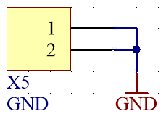
\includegraphics[width=.3\linewidth]{Schuh/Pictures/Basis-masse}}\qquad
    \subfloat[Hardware\label{fig:basisplatine-masse-hard}]{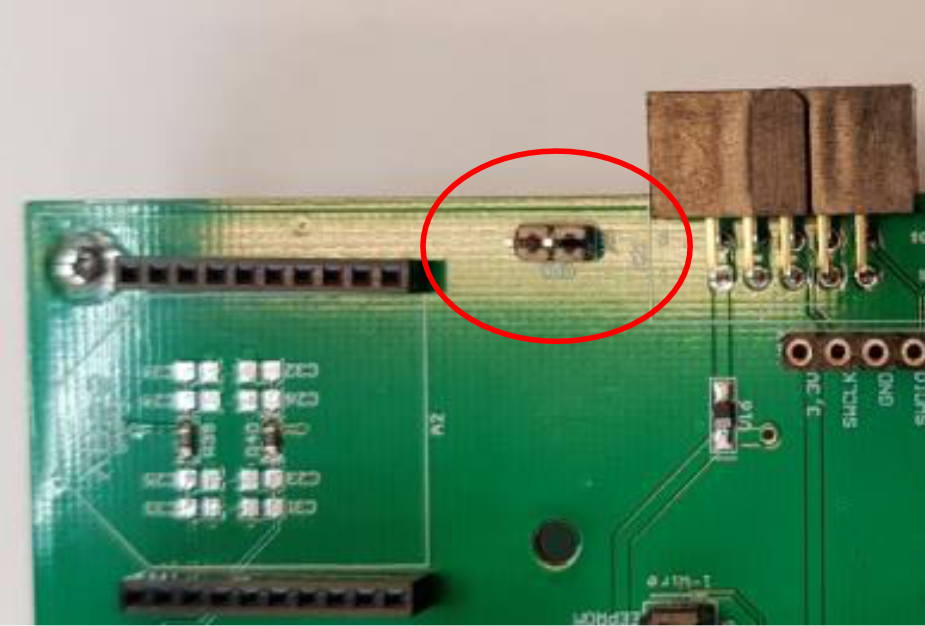
\includegraphics[width=.4\linewidth]{Schuh/Pictures/basis-masse}}\qquad
    \caption[Masseschleife der Basisplatine]{Masseschleife der \gls{Basisplatine}}
    \label{fig:basisplatine-masse}
\end{figure}

\subsubsection{Powerswitch STMPS2141}
Um USB-Geräte zu betreiben, welche selbst keine eigene Spannungsversorgung besitzen (z.B. USB-Sticks) wurde ein Powerswitch D3 (\fref{fig:basisplatine-power}) verbaut. Dieser ermöglicht es die interne \unit{5}{\volt}-Versorgung auf die USB-Buchsen zu legen, damit diese Geräte mit Spannung versorgt werden können. Sollte das Gerät zu viel Strom verbrauchen beginnt die LED V9 (\fref{fig:basisplatine-power}) zu leuchten. Durch Jumpern der Stiftleiste X4 (\fref{fig:basisplatine-power}) an den Port-Pin PC9 kann die Versorgung von externen Geräten gesteuert werden.

\begin{figure}[H]
    \centering
    \subfloat[Schematic\label{fig:basisplatine-power-schem}]{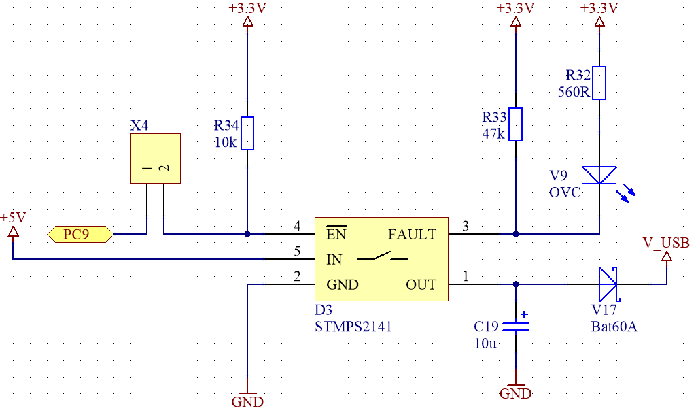
\includegraphics[width=\linewidth]{Schuh/Pictures/Basis-power}}\qquad
    \subfloat[Hardware\label{fig:basisplatine-power-hard}]{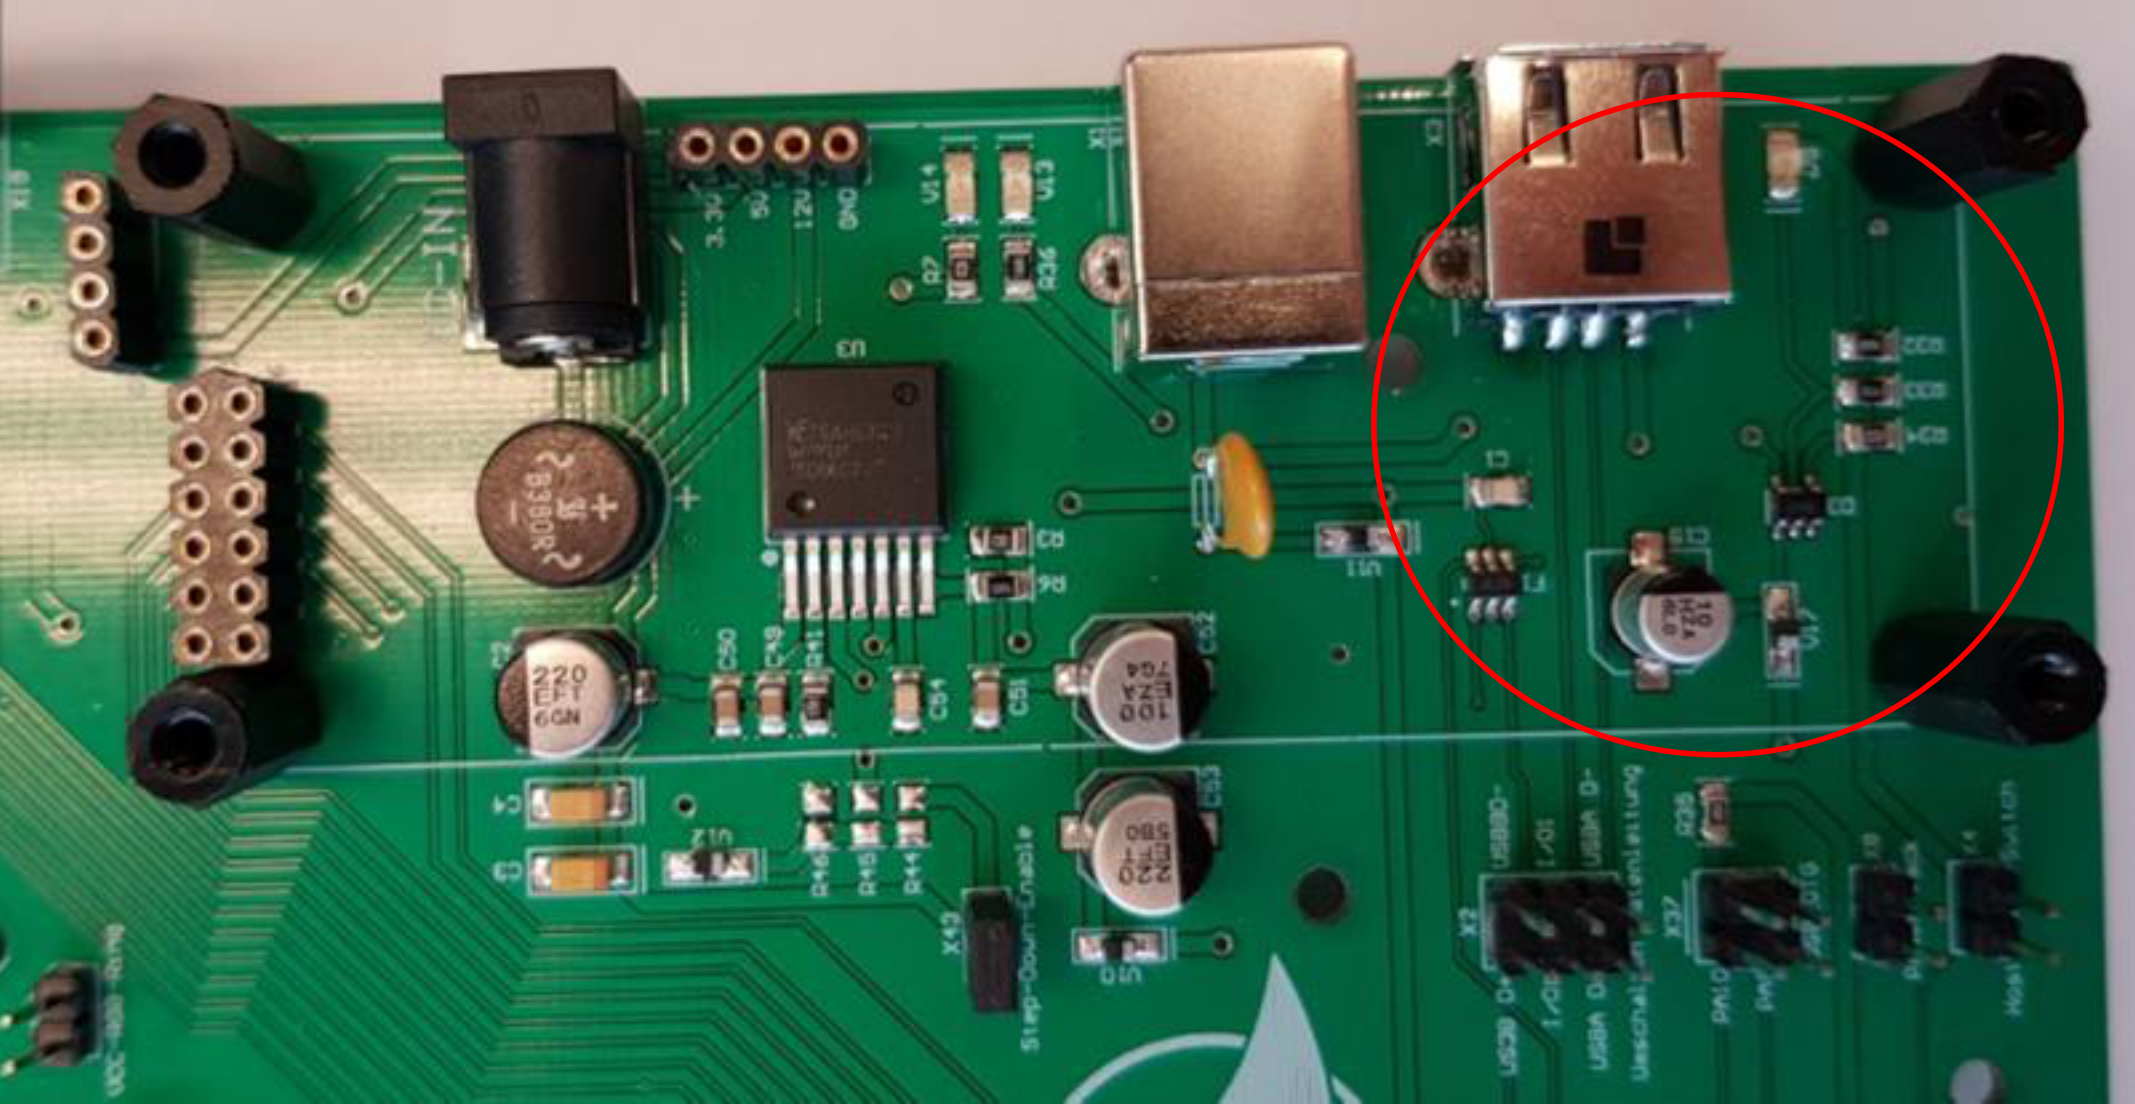
\includegraphics[width=\linewidth]{Schuh/Pictures/basis-power}}\qquad
    \caption[USB Powerswitch der Basisplatine]{USB Powerswitch der \gls{Basisplatine}}
    \label{fig:basisplatine-power}
\end{figure}

\subsubsection{Powerheader}
Um die auf der \gls{Basisplatine} verwendeten Spannungen direkt für Versuchsaufbauten am Steckbrett oder für externe Sensoren verwenden zu können wurden zwei Buchsenleisten X6 und X7 (\fref{fig:basisplatine-pwrhdr}) ausgeführt, welche diese Spannungen bereitstellen. Dabei ist zu beachten, dass am \unit{12}{\volt}-Ausgang nur \unit{+12}{\volt} anliegen, wenn die Basisplatine über ein externes Netzteil mit einer Ausgangsspannung von \unit{+12}{\volt} betrieben wird. Sollte eine geringere Spannung über das Netzgerät eingespeist werden liegt diese am Ausgang an, wenn hingegen kein Netzteil verwendet wird ist dieser Ausgang spannungsfrei.

\begin{figure}[H]
    \centering
    \subfloat[Schematic\label{fig:basisplatine-pwrhdr-schem}]{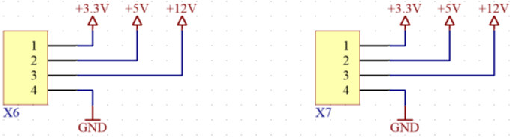
\includegraphics[width=\linewidth]{Schuh/Pictures/Basis-pwrhdr}}\qquad
    \subfloat[Hardware\label{fig:basisplatine-pwrhdr-hard}]{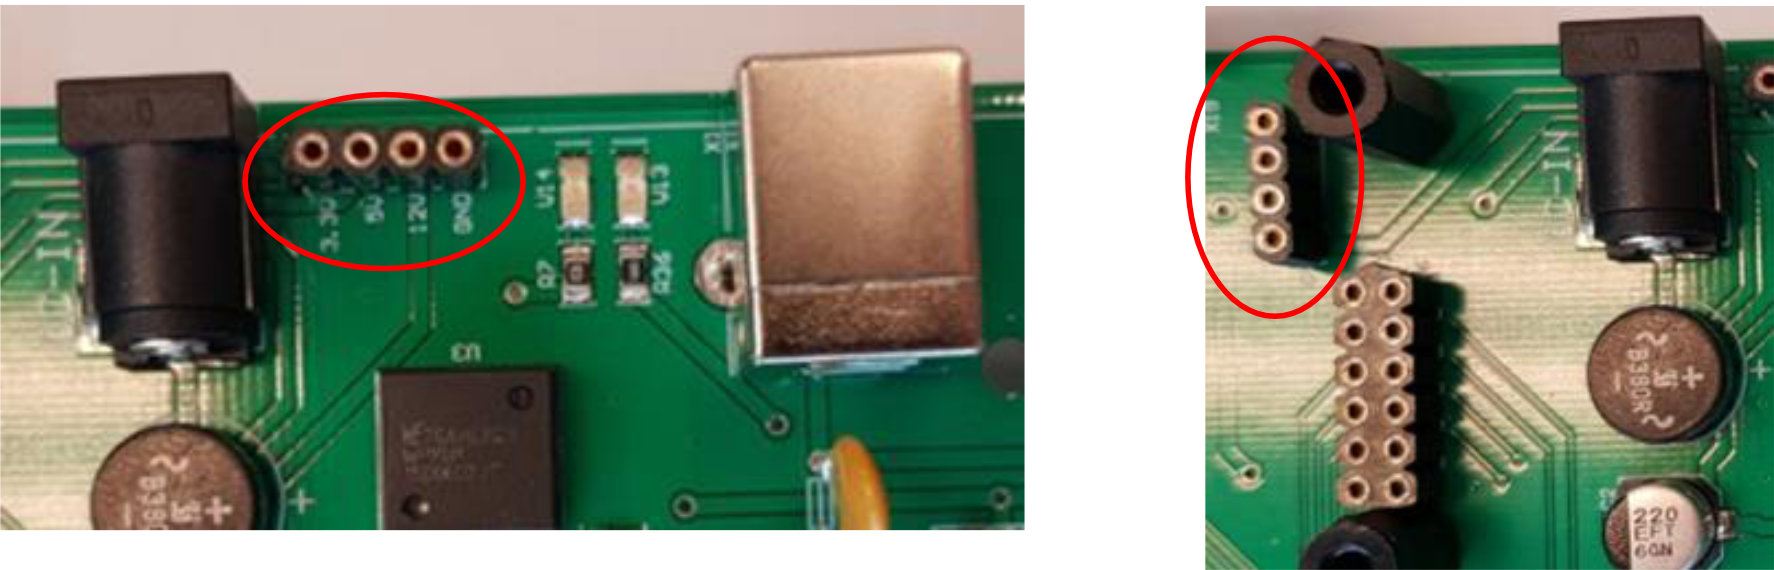
\includegraphics[width=\linewidth]{Schuh/Pictures/basis-pwrhdr}}\qquad
    \caption[Powerheader der Basisplatine]{Powerheader der \gls{Basisplatine}}
    \label{fig:basisplatine-pwrhdr}
\end{figure}

\subsubsection{3,3 V-Versorgung}
Zur Überprüfung ob die \gls{Basisplatine} mit der Betriebsspannung von \unit{+3,3}{\volt} über das \gls{Core-Modul} versorgt wird, wurde die LED V14 (\fref{fig:basisplatine-3v3}) zur optischen Kontrolle eingebaut. Wenn die Basisplatine mit Spannung versorgt wird, beginnt diese zu leuchten.

\begin{figure}[H]
    \centering
    \subfloat[Schematic\label{fig:basisplatine-3v3-schem}]{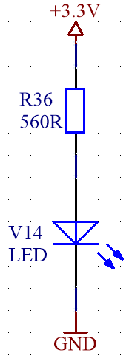
\includegraphics[width=.2\linewidth]{Schuh/Pictures/Basis-3v3}}\qquad
    \subfloat[Hardware\label{fig:basisplatine-3v3-hard}]{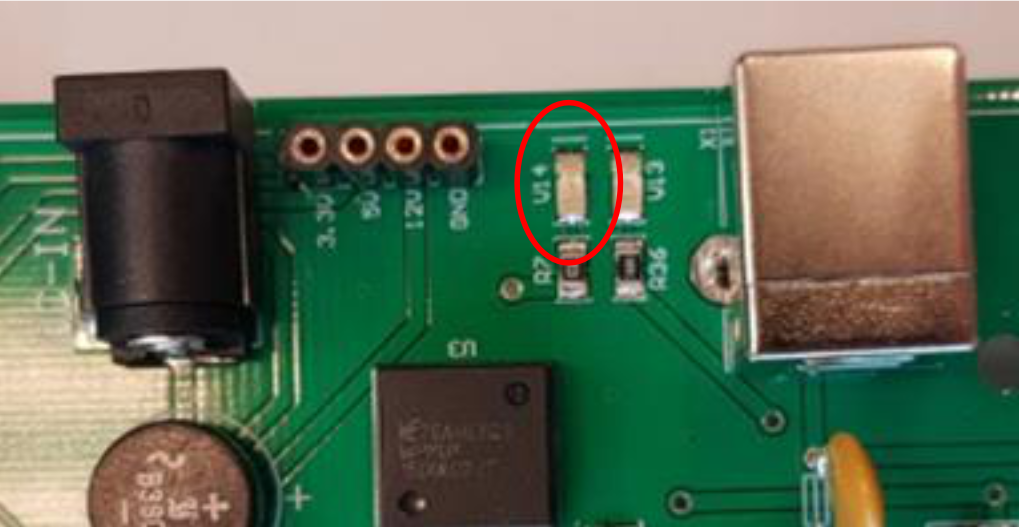
\includegraphics[width=.4\linewidth]{Schuh/Pictures/basis-3v3}}\qquad
    \caption[\unit{3,3}{\volt}-Versorgung der Basisplatine]{\unit{3,3}{\volt}-Versorgung der \gls{Basisplatine}}
    \label{fig:basisplatine-3v3}
\end{figure}

\subsubsection{Spannungsversorgung über DC-Buchse}
Als weitere Spannungsversorgungsmöglichkeit bietet die \gls{Basisplatine} die Möglichkeit ein \unit{9}{\volt} bis \unit{12}{\volt} DC-Netzteil am die DC-Buchse J1 (\fref{fig:basisplatine-dc}) anzuschließen um die Basisplatine mit Spannung zu versorgen. Der Brückengleichrichter U1 (\fref{fig:basisplatine-dc}) dient dabei lediglich als Verpolungsschutz und nicht als Gleichrichter für Wechselspannung. Das Anlegen von Wechselspannung an die DC-Buchse J1 (\fref{fig:basisplatine-dc}) sollte aus Sicherheitsgründen unterlassen werden. Um aus der hohen Spannung, welche von der DC-Buchse kommt, die Betriebsspannung von \unit{+5}{\volt} zu generieren wurde ein Step-Down Modul U3 (\fref{fig:basisplatine-dc}) der Firma Würth verbaut. Zur Überprüfung ob das Step-Down Modul die Betriebsspannung von \unit{+5}{\volt} generiert, wurde die LED V13 (\fref{fig:basisplatine-dc}) zur optischen Kontrolle eingebaut. Wenn das Step-Down Modul die gewünschte Spannung generiert, beginnt diese zu leuchten. Die Stiftleiste X43 (\fref{fig:basisplatine-dc}) kann im Bedarfsfall gejumpert werden, wenn ein Unterspannungsschutz der Versorgungsspannung gewünscht ist. Um die vom Step-Down Modul generierte Spannung verwenden zu können muss lediglich die Stiftleiste X8 (\fref{fig:basisplatine-dc}) mit einem Jumper versehen werden.

\begin{figure}[H]
    \centering
    \subfloat[Schematic\label{fig:basisplatine-dc-schem}]{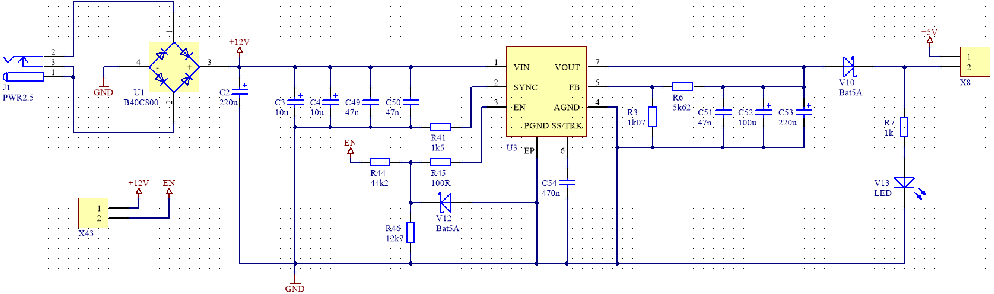
\includegraphics[width=\linewidth]{Schuh/Pictures/Basis-dc}}\qquad
    \subfloat[Hardware\label{fig:basisplatine-dc-hard}]{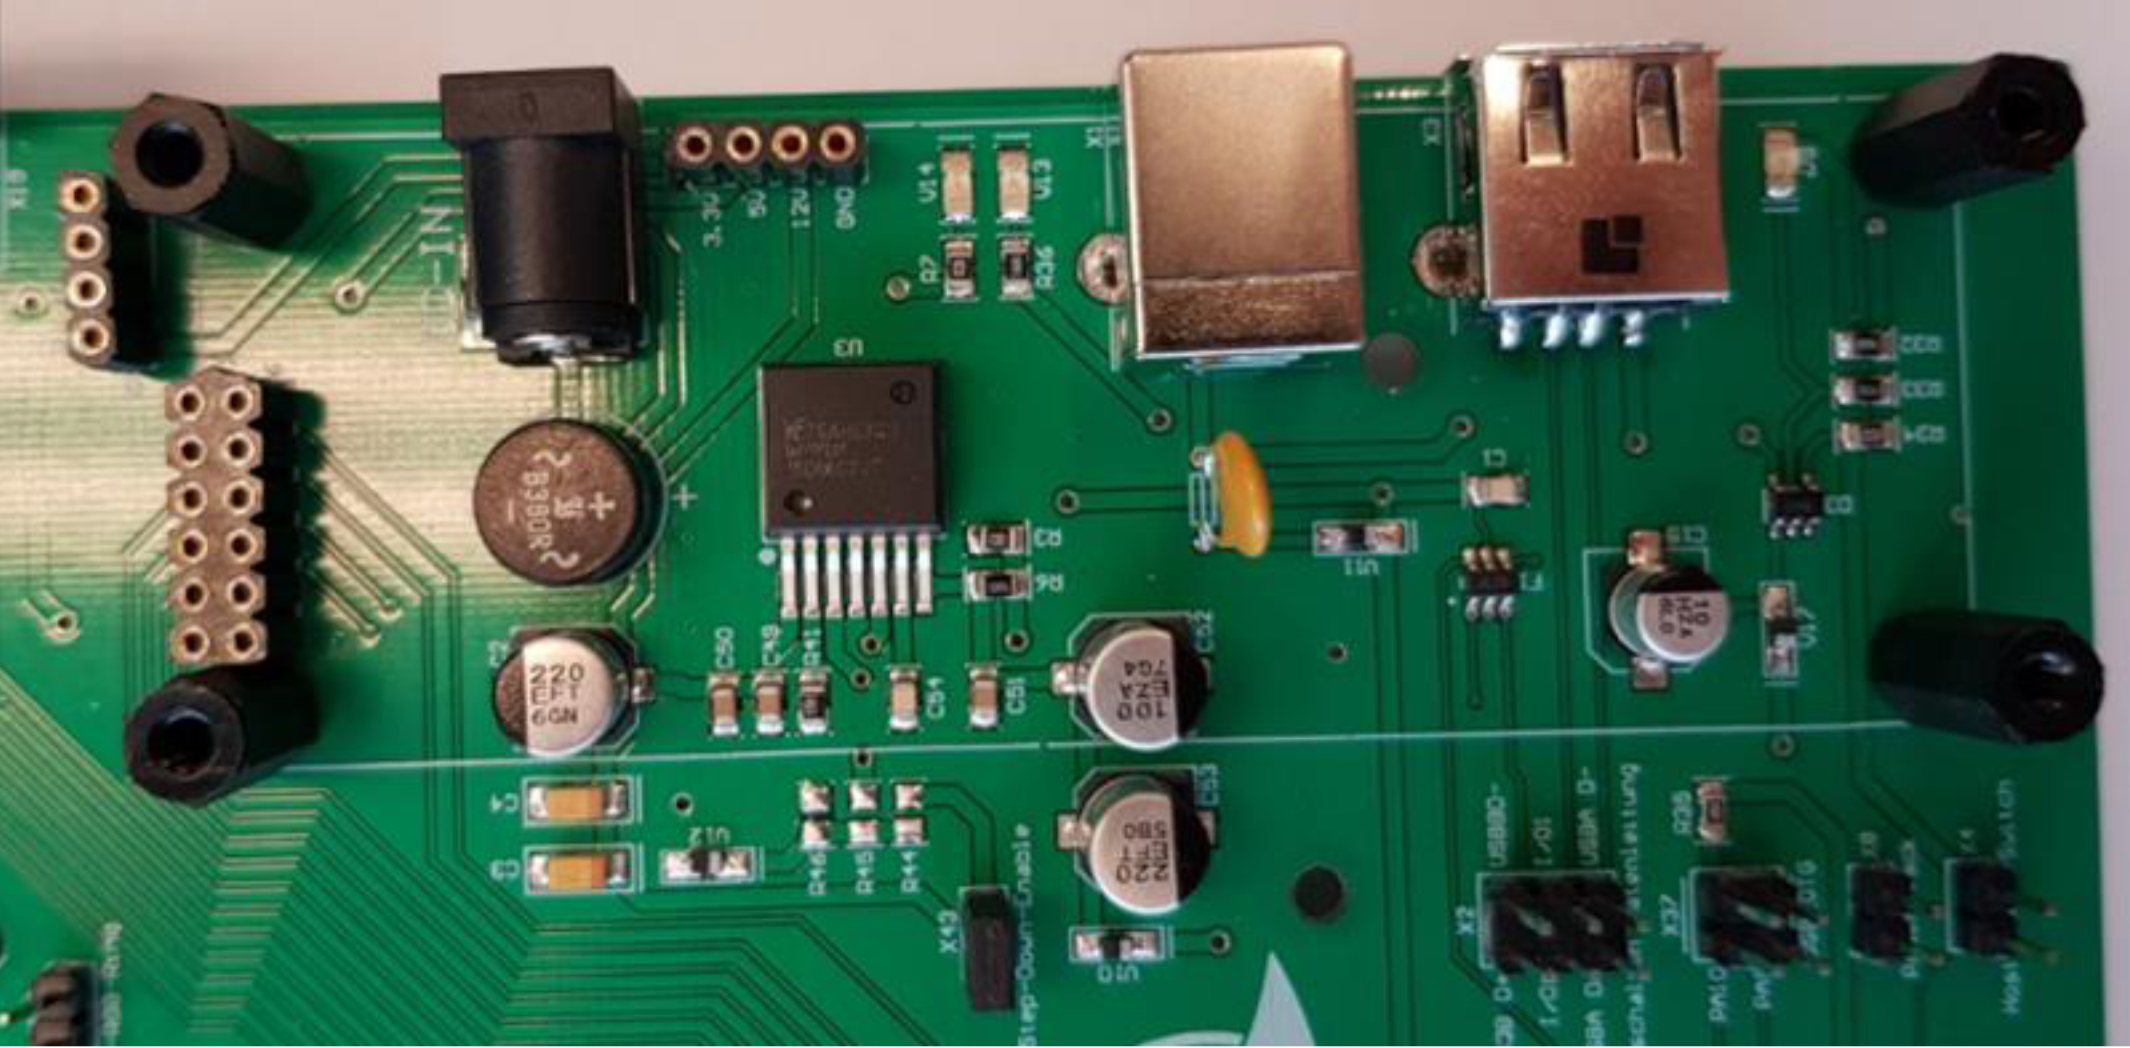
\includegraphics[width=\linewidth]{Schuh/Pictures/basis-dc}}\qquad
    \caption[DC-Versorgung der Basisplatine]{DC-Versorgung der \gls{Basisplatine}}
    \label{fig:basisplatine-dc}
\end{figure}

\subsubsection{RGB-LED Ring \cite{basis:ws2812b}}
Auf der \gls{Basisplatine} wurde ein aus zwölf RGB-LEDs bestehender Ring aufgebaut, welcher in den verschiedensten Farben leuchten kann. Jede RGB-LED besitzt einen eigenen eingebauten Controller. Die Ansteuerung der LEDs wird über den Port-Pin PB0 realisiert. Um diesen verwenden zu können muss zuvor die Stiftleiste X41 (\fref{fig:basisplatine-ledring}) mit einem Jumper versehen werden. Weiters muss die Spannungsversorgung der LEDs gewährleistet sein. Dazu muss lediglich die Stiftleiste X42 (\fref{fig:basisplatine-ledring}) mit einem Jumper versehen werden.

\begin{figure}[H]
    \centering
    \subfloat[Schematic\label{fig:basisplatine-ledring-schem}]{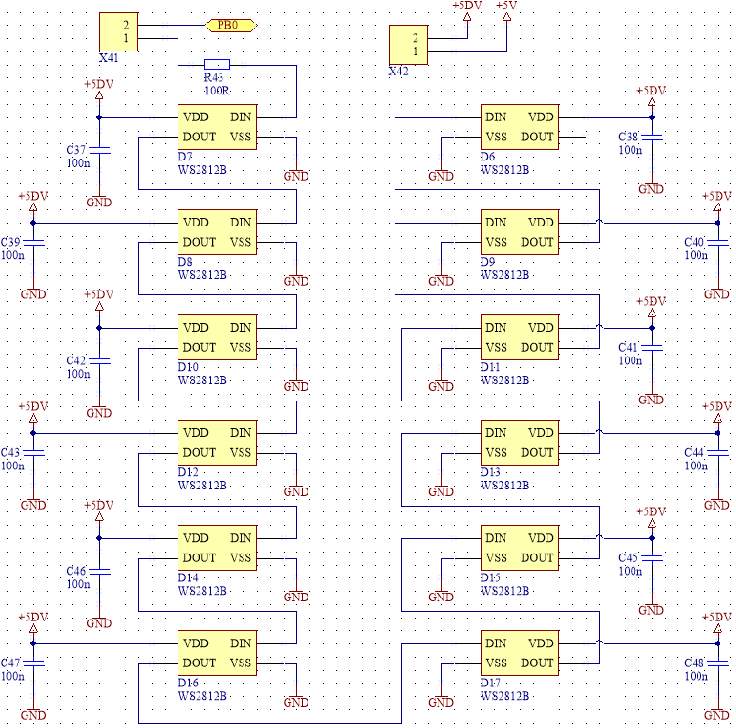
\includegraphics[width=.75\linewidth]{Schuh/Pictures/Basis-ledring}}\qquad
    \subfloat[Hardware\label{fig:basisplatine-ledring-hard}]{\includegraphics[width=.3\linewidth]{Schuh/Pictures/basis-ledring}}\qquad
    \caption[RGB-LED Ring der Basisplatine]{RGB-LED Ring der \gls{Basisplatine}}
    \label{fig:basisplatine-ledring}
\end{figure}

Zur Programmierung der LEDs muss über den Port PB0 ein Datenwort übetragen werden, welches 24 bit pro LED enthält, siehe \fref{fig:basisplatine-ledring-data}. Dies ergibt insgesamt 288 bit, welche übertragen werden müssen. Wie die Übertragung genau aussieht kann aus \fref{fig:basisplatine-ledring-timing} entnommen werden.

\fig{basisplatine-ledring-data}{RGB-LED Ring Datenstruktur}{RGB-LED Ring Datenstruktur \cite{basis:ws2812b}}{\textwidth}{Schuh/Pictures/Basis-ledring-data}
\fig{basisplatine-ledring-timing}{RGB-LED Ring Timing Diagram}{RGB-LED Ring Timing Diagram \cite{basis:ws2812b}}{\textwidth}{Schuh/Pictures/Basis-ledring-timing}

Die Daten für jede LED im Ring werden seriell hintereinander wie in \fref{fig:basisplatine-ledring-data} beschrieben übertragen, hierbei wird zuerste die erste LED angesprochen, wenn diese die richtigen Daten hat, leitet sie alle weiteren Datenpakete transparent weiter, sodass danach die zweite LED angesprochen wird und so weiter, bis ein Reset Code (\unit{50}{\micro\second} oder länger \enquote{High}) gesendet wird. Danach kann wieder die erste LED angesprochen werden. das genau Timing kann hierbai aus dem Datenblatt \cite{basis:ws2812b} entnommen werden.

\subsubsection{Sensor-Selektion}
Da der verbaute Prozessor zu wenig Portleitungen besitzt um alle Sensoren und Module mit einer eigenen Portleitung zu versorgen, werden einige Portleitungen mehrmals verwendet. Um nun einzelne Module oder Sensoren verwenden zu können, müssen diese einsprechend gejumpert werden. Eine dieser Stiftleisten ist der Header X9 (\fref{fig:basisplatine-ssel}), welches es ermöglicht zwischen einem Potentiometer (\gls{ADC}), Piezo-Summer, einem LFU, einem Infrarotempfänger, einem Temperaturfühler und einem NE555 auszuwählen.

Eine weitere dieser Stiftleisten ist der Header X11 (\fref{fig:basisplatine-ssel2}), welche es ermöglicht zwischen dem Beschleunigungssensor und dem EEPROM auszuwählen.

\begin{figure}[H]
    \centering
    \subfloat[Schematic\label{fig:basisplatine-ssel-schem}]{\includegraphics[width=.5\linewidth]{Schuh/Pictures/Basis-ssel}}\qquad
    \subfloat[Hardware\label{fig:basisplatine-ssel-hard}]{\includegraphics[width=.3\linewidth]{Schuh/Pictures/basis-ssel}}\qquad
    \caption[Sensor-Selektion der Basisplatine]{Sensor-Selektion der \gls{Basisplatine}}
    \label{fig:basisplatine-ssel}
\end{figure}

\begin{figure}[H]
    \centering
    \subfloat[Schematic\label{fig:basisplatine-ssel2-schem}]{\includegraphics[width=.5\linewidth]{Schuh/Pictures/Basis-ssel2}}\qquad
    \subfloat[Hardware\label{fig:basisplatine-ssel2-hard}]{\includegraphics[width=.3\linewidth]{Schuh/Pictures/basis-ssel2}}\qquad
    \caption[Sensor-Selektion der Basisplatine]{Sensor-Selektion der \gls{Basisplatine}}
    \label{fig:basisplatine-ssel2}
\end{figure}

\subsubsection{Piezo-Summer}
Auf der \gls{Basisplatine} wurde ein Piezo-Summer B4 (\fref{fig:basisplatine-piezo}) verbaut, welcher über den Port-Pin PB0 angesteuert werden kann. Ja nach anliegender Taktfrequenz am Eingang des Summers wird der erzeugte Ton höher oder tiefer. Um den Piezo-Summer verwenden zu können muss lediglich der Pin11 mit dem Pin12, der zweireihige Stiftleiste X9 (\fref{fig:basisplatine-ssel}), gejumpert werden.

\begin{figure}[H]
    \centering
    \subfloat[Schematic\label{fig:basisplatine-piezo-schem}]{\includegraphics[width=.5\linewidth]{Schuh/Pictures/Basis-piezo}}\qquad
    \subfloat[Hardware\label{fig:basisplatine-piezo-hard}]{\includegraphics[width=.3\linewidth]{Schuh/Pictures/basis-piezo}}\qquad
    \caption[Piezo-Summer der Basisplatine]{Piezo-Summer der \gls{Basisplatine}}
    \label{fig:basisplatine-piezo}
\end{figure}

\subsubsection{Potentiometer}
Es wurden zwei Potentiometer R9 und R4 hardwaremäßig auf der \gls{Basisplatine} vorgesehen. Diese sind direkt mit einem \gls{ADC}-Eingang des Prozessors verbunden. Der Unterschied zwischen den Potentiometern R9 und R4 besteht darin, dass das Potentiometer R4 über einen Jumper auf der Stiftleiste X40 (\fref{fig:basisplatine-poti2-schem}) aktiviert werden muss und dieses an einem anderen Port-Pin angeschlossen ist. Dieser Aufbau wurde deswegen gewählt da damit, damit an den \gls{ADC}-Eingang auch optional ein anderes Signal angelegt werden kann. 

\begin{figure}[H]
    \centering
    \subfloat[Schematic\label{fig:basisplatine-poti1-schem}]{\includegraphics[width=.4\linewidth]{Schuh/Pictures/Basis-poti1}}\qquad
    \subfloat[Schematic\label{fig:basisplatine-poti2-schem}]{\includegraphics[width=.4\linewidth]{Schuh/Pictures/Basis-poti2}}\qquad
    \subfloat[Hardware\label{fig:basisplatine-poti-hard}]{\includegraphics[width=.4\linewidth]{Schuh/Pictures/basis-poti}}\qquad
    \caption[Potentiometer der Basisplatine]{Potentiometer der \gls{Basisplatine}}
    \label{fig:basisplatine-poti}
\end{figure}

\subsubsection{EEPROM}
Um Daten permanent speichern zu können wurde das EEPROM D1 (\fref{fig:basisplatine-eeprom}) vorgesehen. Standardmäßig wird das EEPROM 24AA256 verwendet, welches es ermöglicht 256 kbit abzuspeichern. Dieses EEPROM besitzt eine Write-Protection WP welche es ermöglicht das EEPROM schreibgeschützt zu schalten. Die Write-Protection kann über die Portleitung PB5 gesteuert werden. Damit das Signal am EEPROM ankommt, muss jedoch der Pin3 mit dem Pin4 der zweireihigen Stiftleiste X11 (\fref{fig:basisplatine-ssel2}) gejumpert werden. Die Kommunikation mit dem EEPROM erfolgt über den \IIC{}-Bus (Adresse \texttt{0xA0}).

\begin{figure}[H]
    \centering
    \subfloat[Schematic\label{fig:basisplatine-eeprom-schem}]{\includegraphics[width=.5\linewidth]{Schuh/Pictures/Basis-eeprom}}\qquad
    \subfloat[Hardware\label{fig:basisplatine-eeprom-hard}]{\includegraphics[width=.3\linewidth]{Schuh/Pictures/basis-eeprom}}\qquad
    \caption[EEPROM der Basisplatine]{EEPROM der \gls{Basisplatine}}
    \label{fig:basisplatine-eeprom}
\end{figure}

\subsubsection{Beschleunigungssensor}
Auf der \gls{Basisplatine} wurde auch ein Beschleunigungssensormodul mit dem Beschleunigungssensor BMA020 vorgesehen. Die Kommunikation mit dem Beschleunigungssensor erfolgt mit Hilfe des \IIC{}-Buses (Adresse \texttt{0x70}). Durch diesen Sensor kann die Neigung, sowie die Kraft welche auf die Platine wirkt in der X, Y und Z-Richtung erfasst werden. Der Beschleunigungssensor besitzt einen Interrupt-Pin, welcher es ermöglicht ein Interrupt auszulösen. Der Interrupt kann über die Portleitung PB5 empfangen werden. Damit das Interrupt-Signal an der Portleitung PB5 ankommt, muss jedoch der Pin1 mit dem Pin2 der zweireihigen Stiftleiste X11 (\fref{fig:basisplatine-ssel2}) gejumpert werden.

\begin{figure}[H]
    \centering
    \subfloat[Schematic\label{fig:basisplatine-bma-schem}]{\includegraphics[width=.5\linewidth]{Schuh/Pictures/Basis-bma}}\qquad
    \subfloat[Hardware\label{fig:basisplatine-bma-hard}]{\includegraphics[width=.3\linewidth]{Schuh/Pictures/basis-bma}}\qquad
    \caption[Beschleunigungssensor der Basisplatine]{Beschleunigungssensor der \gls{Basisplatine}}
    \label{fig:basisplatine-bma}
\end{figure}

\subsubsection{IR-Receiver}
Um die Platine auch mit einer Fernbedienung oder einem Mobiltelefon steuern zu können würde ein IR-Receiver verbaut. Dieser Sensor wurde hardwaremäßig unter dem NEXTION-Display angebracht. Der IR-Receiver arbeitet mit einer Wellenlänge von 850nm bis 1000nm und einer Trägerfrequenz von 38kHz. Das vom IR-Receiver empfangene Signal wird direkt im Receiver demoduliert und anschließend zur Stiftleiste X9 (\fref{fig:basisplatine-ssel}) weitergeleitet. Um den IR-Receiver verwenden zu können muss lediglich der Pin7 mit dem Pin8, der Stiftleiste X9 (\fref{fig:basisplatine-ssel}), gejumpert werden.

\begin{figure}[H]
    \centering
    \subfloat[Schematic\label{fig:basisplatine-ir-schem}]{\includegraphics[width=.5\linewidth]{Schuh/Pictures/Basis-ir}}\qquad
    \subfloat[Hardware\label{fig:basisplatine-ir-hard}]{\includegraphics[width=.3\linewidth]{Schuh/Pictures/basis-ir}}\qquad
    \caption[IR-Receiver der Basisplatine]{IR-Receiver der \gls{Basisplatine}}
    \label{fig:basisplatine-ir}
\end{figure}

\subsubsection{Temperatursensor}
Um die Umgebungstemperatur feststellen zu können wurde auf der Basisplatine der Temperaturfühler DS18B20 verbaut, welcher mit Hilfe des 1-Wire Protokolls angesprochen werden kann. Die maximale Mesfehler dieses Temperatursensors beträgt ±0,5°C laut Datenblattangabe. Um den Temperaturfühler verwenden zu können muss lediglich der Pin9 mit dem Pin10, der Stiftleiste X9 (\fref{fig:basisplatine-ssel}), gejumpert werden. 

\begin{figure}[H]
    \centering
    \subfloat[Schematic\label{fig:basisplatine-temp-schem}]{\includegraphics[width=.5\linewidth]{Schuh/Pictures/Basis-temp}}\qquad
    \subfloat[Hardware\label{fig:basisplatine-temp-hard}]{\includegraphics[width=.3\linewidth]{Schuh/Pictures/basis-temp}}\qquad
    \caption[Temperatursensor der Basisplatine]{Temperatursensor der \gls{Basisplatine}}
    \label{fig:basisplatine-temp}
\end{figure}

\subsubsection{Lichtwandler LFU}
Der auf der \gls{Basisplatine} realisierte LFU (Licht-Frequenz-Wandler), wandeltet wie der Name bereits sagt Licht in eine bestimmte Frequenz um. Je höher die Bestrahlungsstärke des Lichts, desto höher wird die über den Output des LFUs ausgegebene Frequenz. Den linearen Zusammenhang zwischen der Bestrahlungsstärke und der ausgegebenen Frequenz kann aus \fref{fig:basisplatine-lfu-freq} entnommen werden. Um den LFU verwenden zu können muss lediglich der Pin5 mit dem Pin6, der Stiftleiste X9 (\fref{fig:basisplatine-ssel}), gejumpert werden.

\begin{figure}[H]
    \centering
    \subfloat[Schematic\label{fig:basisplatine-lfu-schem}]{\includegraphics[width=.5\linewidth]{Schuh/Pictures/Basis-lfu}}\qquad
    \subfloat[Hardware\label{fig:basisplatine-lfu-hard}]{\includegraphics[width=.3\linewidth]{Schuh/Pictures/basis-lfu}}\qquad
    \caption[LFU der Basisplatine]{LFU der \gls{Basisplatine}}
    \label{fig:basisplatine-lfu}
\end{figure}
\fig{basisplatine-lfu-freq}{Frequenzgang des LFUs}{Frequenzgang des LFUs}{0.5\textwidth}{Schuh/Pictures/Basis-lfu-freq}

\subsubsection{RGB-LED}
Auf der \gls{Basisplatine} wurde ebenso eine RGB-LED \cite{basis:rgbled} verbaut, welche mit Hilfe des LED-Drivers D4 (\fref{fig:basisplatine-rgbled}) \cite{basis:rgbdriver}, welcher mit dem \IIC{}-Bus (Adresse \texttt{0x70}) angesteuert werden kann. Dieser LED-Driver hat den Vorteil, dass er eine interne Stromüberwachung besitzt. Dadurch benötigen die einzelnen Anoden der RGB-LED keine Vorwiderstände, da sich der Strom automatisch entsprechend der gewünschten Farbe reguliert.

\begin{figure}[H]
    \centering
    \subfloat[Schematic\label{fig:basisplatine-rgbled-schem}]{\includegraphics[width=.5\linewidth]{Schuh/Pictures/Basis-rgbled}}\qquad
    \subfloat[Hardware\label{fig:basisplatine-rgbled-hard}]{\includegraphics[width=.3\linewidth]{Schuh/Pictures/basis-rgbled}}\qquad
    \caption[RGB-LED der Basisplatine]{RGB-LED der \gls{Basisplatine}}
    \label{fig:basisplatine-rgbled}
\end{figure}
\fig{basisplatine-rgbled-befehl}{Befehlsaufbau der RGB-LED}{Befehlsaufbau der RGB-LED \cite{basis:rgbdriver}}{\textwidth}{Schuh/Pictures/Basis-rgbled-befehl}
\fig{basisplatine-rgbled-register}{Register der RGB-LED}{Register der RGB-LED \cite{basis:rgbdriver}}{\textwidth}{Schuh/Pictures/Basis-rgbled-register}
\fig{basisplatine-rgbled-seq}{Sequenzen der RGB-LED}{Sequenzen der RGB-LED \cite{basis:rgbdriver}}{\textwidth}{Schuh/Pictures/Basis-rgbled-seq}

\subsubsection{Arduino-Shield-Header}
Um Hardware des Arduino-Mikrocontrollersystems nutzten zu können, ohne selbst großen Aufwand in die Entwicklung entsprechender Module investieren zu müssen, wurde ein Arduino-Shield-Header auf der \gls{Basisplatine} vorgesehen. Dieser ermöglicht es durch die Portkompatibilität mit einem Arduino, dessen Shields zu verwenden oder selbst Shields entwickeln zu können. Möchte man nun ein Arduino-Shield verwenden muss dieses lediglich in die vorgesehene Buchsenleiste X33 (\fref{fig:basisplatine-arduino}) gesteckt werden. Da jedes Arduino-Shield die Möglichkeit besitzt eine Referenzspannung für diverse ADCs zu vergeben wurde das Potentiometer R31 vorgesehen, um diesen Spannungspegel variabel zu gestallten. Darüber hinaus gibt es noch die Möglichkeit bei speziellen Shields zu definieren mit welcher Betriebsspannung die darüberliegenden versorgt werden sollen. Dazu wurde die Stiftleiste X27 verbaut, um festzulegen ob die darüberliegenden Shields mit \unit{+5}{\volt} oder \unit{+3,3}{\volt} versorgt werden. Sollte kein Jumper gesetzt werden wird automatisch auf die \unit{+5}{\volt} Spannungsversorgung zurückgegriffen.

\begin{figure}[H]
    \centering
    \subfloat[Schematic\label{fig:basisplatine-arduino-schem}]{\includegraphics[width=.5\linewidth]{Schuh/Pictures/Basis-arduino}}\qquad
    \subfloat[Hardware\label{fig:basisplatine-arduino-hard}]{\includegraphics[width=.3\linewidth]{Schuh/Pictures/basis-arduino}}\qquad
    \caption[Arduino-Shield-Header der Basisplatine]{Arduino-Shield-Header der \gls{Basisplatine}}
    \label{fig:basisplatine-arduino}
\end{figure}

\subsubsection{WLAN-Modul \cite{basis:wlan}}
Um Daten ohne großen Aufwand direkt in das Heimnetzwerk einspeisen zu können, wurde auf der auf der \gls{Basisplatine} ein Steckplatz X35 (\fref{fig:basisplatine-wlan}) für ein ESP8266 W-LAN Modul vorgesehen. Dieses Funkmodul benutzt zu Kommunikation mit dem Prozessor des Core-Moduls die UART2 Schnittstelle und sendet die Daten mit einer Sendefrequenz von \unit{2,4}{\giga\hertz} im ISM-Band. Wenn man die Firmware des ESP8266 verändern möchte muss man lediglich die Portleitung GPIO0 des ESP8266, durch jumpern von Pin2 und Pin3 der Stiftleiste X39 (\fref{fig:basisplatine-wlan}), gegen Masse schalten.

\begin{figure}[H]
    \centering
    \subfloat[Schematic\label{fig:basisplatine-wlan-schem}]{\includegraphics[width=.5\linewidth]{Schuh/Pictures/Basis-wlan}}\qquad
    \subfloat[Hardware\label{fig:basisplatine-wlan-hard}]{\includegraphics[width=.3\linewidth]{Schuh/Pictures/basis-wlan}}\qquad
    \caption[WLAN-Modul der Basisplatine]{WLAN-Modul der \gls{Basisplatine}}
    \label{fig:basisplatine-wlan}
\end{figure}

\subsubsection{XBee-Pro-Modul}
Um Daten ohne großen Aufwand per Funk übertragen können, wurde auf der auf der \gls{Basisplatine} ein Steckplatz A2 (\fref{fig:basisplatine-xbee}) für ein XBee-Pro Modul vorgesehen. Dieses Funkmodul benutzt zu Kommunikation mit dem Prozessor des \gls{Core-Modul}s die UART2 Schnittstelle und sendet die Daten mit einer Sendefrequenz von \unit{2,4}{\giga\hertz} im ISM-Band. Darüber hinaus weist das Funkmodul eine maximale Datenübertragungsrate von 250 kb/s auf und hat eine maximale Reichweite von \unit{1600}{\metre}.

\begin{figure}[H]
    \centering
    \subfloat[Schematic\label{fig:basisplatine-xbee-schem}]{\includegraphics[width=.5\linewidth]{Schuh/Pictures/Basis-xbee}}\qquad
    \subfloat[Hardware\label{fig:basisplatine-xbee-hard}]{\includegraphics[width=.3\linewidth]{Schuh/Pictures/basis-xbee}}\qquad
    \caption[XBee-Pro-Modul der Basisplatine]{XBee-Pro-Modul der \gls{Basisplatine}}
    \label{fig:basisplatine-xbee}
\end{figure}

\subsubsection{HC-06-Modul \cite{basis:hc06}}
Um Daten ohne großen Aufwand per Bluetooth übertragen können, wurde auf der auf der \gls{Basisplatine} ein Steckplatz X28 (\fref{fig:basisplatine-hc06}) für ein HC-06 Bluetooth-Modul vorgesehen. Dieses Bluetooth-Modul benutzt zur Kommunikation mit dem Prozessor des \gls{Core-Modul}s die UART1 Schnittstelle und sendet die Daten mit einer Sendefrequenz von \unit{2,4}{\giga\hertz} im ISM-Band. Darüber hinaus weist das Bluetooth-Modul eine maximale Datenübertragungsrate von 1382400 baud auf.

\begin{figure}[H]
    \centering
    \subfloat[Schematic\label{fig:basisplatine-hc06-schem}]{\includegraphics[width=.5\linewidth]{Schuh/Pictures/Basis-hc06}}\qquad
    \subfloat[Hardware\label{fig:basisplatine-hc06-hard}]{\includegraphics[width=.3\linewidth]{Schuh/Pictures/basis-hc06}}\qquad
    \caption[HC-06-Modul der Basisplatine]{HC-06-Modul der \gls{Basisplatine}}
    \label{fig:basisplatine-hc06}
\end{figure}

\subsubsection{HC-12-Modul \cite{basis:hc12}}
Um Daten ohne großen Aufwand per Funk übertragen können, wurde auf der auf der \gls{Basisplatine} ein Steckplatz X31 (\fref{fig:basisplatine-hc12}) für ein HC-12 Funkmodul vorgesehen. Dieses Funkmodul benutzt zu Kommunikation mit dem Prozessor des \gls{Core-Modul}s die UART1 Schnittstelle und sendet die Daten mit einer Sendefrequenz von \unit{433,4}{\mega\hertz} bis \unit{473,0}{\mega\hertz} im ISM-Band. Darüber hinaus weist das Funkmodul eine maximale Datenübertragungsrate von 115200 baud auf und hat eine maximale Reichweite von \unit{1800}{\metre}. Das HC-12 Funkmodul kann mittels AT-Befehlen konfiguriert werden. Dabei kann die maximale Ausgangsleistung, die Sendefrequenz und die maximale Datenübertragungsrate verändert werden.

\begin{figure}[H]
    \centering
    \subfloat[Schematic\label{fig:basisplatine-hc12-schem}]{\includegraphics[width=.5\linewidth]{Schuh/Pictures/Basis-hc12}}\qquad
    \subfloat[Hardware\label{fig:basisplatine-hc12-hard}]{\includegraphics[width=.3\linewidth]{Schuh/Pictures/basis-hc12}}\qquad
    \caption[HC-12-Modul der Basisplatine]{HC-12-Modul der \gls{Basisplatine}}
    \label{fig:basisplatine-hc12}
\end{figure}

Um das Modul in den Programming-Mode zu setzen, müssen folgende Schritte ausgeführt werden:
\begin{itemize}
    \item Um das Modul programmieren zu können muss der Pin5 (\enquote{SET}) gegen Masse gezogen werden, während das Modul mit Spannung versorgt ist (ca. \unit{40}{\milli\second}).
    \item Anschließend muss die Spannungsversorgung unterbrochen werden und der Pin5 (\enquote{SET}) wieder mit Masse verbunden werden. Erst wenn der SET-Pin mit Masse verbunden ist darf das Modul wieder mit Spannung versorgt werden.
\end{itemize}

\ltab{basisplatine-hc12-atbefehlsaufbau}{Aufbau von AT-Befehlen}{Aufbau von AT-Befehlen \cite{basis:hc12}}{|c|p{10cm}|}{
    \hline
    \textbf{Befehl} & \textbf{Funktion}\\
    \hline
    AT & \enquote{AT} ist ein Test-Befehl um festzustellen ob eine Programmierung des Modules möglich ist. Sollte diese möglich sein antwortet das Modul mit \enquote{OK}.\\
    \hline
    AT+B\texttt{xxxx} & Mit diesem Befehl kann die Baudrate des Funkmoduls verändert werden. Anstelle der \enquote{\texttt{x}} gehört die gewünschte Baudrate eingetragen. Sollte der Befehl korrekt an das Funkmodul weitergegeben worden sein antwortet dieses mit \enquote{OK+B\texttt{xxxx}}.\\
    \hline
    AT+C\texttt{xxxx} & Mit diesem Befehl kann der Kommunikationskanal des Funkmoduls verändert werden. Anstelle der \enquote{\texttt{x}} gehört der gewünschte Kommunikationskanal eingetragen. Sollte der Befehl korrekt an das Funkmodul weitergegeben worden sein antwortet dieses mit \enquote{OK+C\texttt{xxxx}}.\\
    \hline
    AT+FU\texttt{x} & Mit diesem Befehl kann der Strombedarf des Funkmoduls verändert werden. Anstelle des \enquote{\texttt{x}} gehört der gewünschte Strombedarf eingetragen. Sollte der Befehl korrekt an das Funkmodul weitergegeben worden sein antwortet dieses mit \enquote{OK+FU\texttt{x}}.\\
    \hline
    AT-P\texttt{x} & Mit diesem Befehl kann die maximale Sendeleistung des Funkmoduls verändert werden. Anstelle des \enquote{\texttt{x}} gehört die gewünschte maximale Sendeleistung eingetragen. Sollte der Befehl korrekt an das Funkmodul weitergegeben worden sein antwortet dieses mit \enquote{OK-P\texttt{x}}.\\
    \hline
    AT-R\texttt{y} & Mit diesem Befehl kann man die aktuellen Einstellungen des Funkmoduls abfragen. Anstelle des \enquote{\texttt{x}} gehört einer der Buchstaben der AT-Befehle (B, C, F, P) eingetragen. Sollte der Befehl korrekt an das Funkmodul weitergegeben worden sein antwortet dieses mit \enquote{OK-R\texttt{y}}.\\
    \hline
    AT+Udps & Mit diesem Befehl können die Anzahl der Datenbits (d), der Paritybits (p) und der Stoppbits (s) verändert werden. Sollte der Befehl korrekt an das Funkmodul weitergegeben worden sein antwortet dieses mit \enquote{OK+Upds}.\\
    \hline
    AT-V & Mit diesem Befehl kann die aktuelle Firmwareversion des Funkmoduls abgefragt werden.\\
    \hline
}
\tabpdf{basisplatine-hc12-at}{HC-12 AT-Befehlsparameter}{Übersicht über die HC-12 AT-Befehlsparameter \cite{basis:hc12}}{\textwidth}{Schuh/Pictures/Basis-hc12-at}

Um das Funkmodul auf Werkseinstellungen zurückzusetzen muss der AT-Befehl \enquote{AT+DEFAULT} eingegeben werden. Sollte der Befehl korrekt an das Funkmodul weitergegeben worden sein antwortet dieses mit \enquote{OK+DEFAULT}. Um die Firmware des Funkmoduls zu updaten muss der AT-Befehl \enquote{AT+UPDATE} eingegeben werden.

\subsubsection{PI-Filter}
Da die \gls{Basisplatine} auf die Verwendung von Funkmodulen ausgelegt ist, welche im HF-Bereich senden und empfangen, wurden als Vorsichtsmaßname PI-Filter für die RX- und TX-Leitungen der UARTs, welche mit den Funkmodulen verbunden sind, vorgesehen um HF-Störungen zu unterdrücken. Je nach Bedarfsfall können nun diese PI-Filter bestückt werden. Im laufendem Betrieb hat sich jedoch gezeigt, dass diese nicht unbedingt erforderlich sind.

\fig{basisplatine-pi}{PI-Filter der Basisplatine}{PI-Filter der \gls{Basisplatine}}{\textwidth}{Schuh/Pictures/Basis-pi}

\subsubsection{NEXTION-Display}
Um den Benutzer eine grafische Darstellungsmöglichkeit von Messwerten, Bildern oder ähnlichen zu geben wurde auf der Basisplatine der Header X25 (\fref{fig:basisplatine-nextion}) vorgesehen. Mit Hilfe dieses Headers ist es möglich ein NEXTION-Display auf der Basisplatine zu befestigen und über die UART3-Schnittstelle anzusteuern. Um das NEXTION-Display verwenden zu können muss lediglich die beiden Pins der Stiftleiste X38 (\fref{fig:basisplatine-nextion}) mit einem Jumper verbunden werden. Zur Programmierung des \gls{GUI}, des NEXTION-Displays wird der selbst entwickelte \gls{USB-to-UART}-Adapter benutzt, welcher in \fref{sec:usbtouart} näher erklärt wird.

\begin{figure}[H]
    \centering
    \subfloat[Schematic\label{fig:basisplatine-nextion-schem}]{\includegraphics[width=.5\linewidth]{Schuh/Pictures/Basis-nextion}}\qquad
    \subfloat[Hardware\label{fig:basisplatine-nextion-hard}]{\includegraphics[width=.3\linewidth]{Schuh/Pictures/basis-nextion}}\qquad
    \caption[NEXTION-Display der Basisplatine]{NEXTION-Display der \gls{Basisplatine}}
    \label{fig:basisplatine-nextion}
\end{figure}

\subsubsection{SPI-Schnittstelle}
Um zusätzliche Hardware mit der \gls{Basisplatine} ansteuern zu können wurde die SPI-Schnittstelle X30 (\fref{fig:basisplatine-spi}) vorgesehen, welche mit der SPI2-Schnitstelle des Prozessors verbunden ist. Da die Chip-Select Leitung (CS) von keiner Hardware auf der Basisplatine benötigt wird, kann diese verwendet werden. Sollten jedoch mehrere Geräte an den SPI-Bus angeschlossen werden, müssen weitere Portleitungen als Chip-Select Leitungen verwendet werden.

\begin{figure}[H]
    \centering
    \subfloat[Schematic\label{fig:basisplatine-spi-schem}]{\includegraphics[width=.5\linewidth]{Schuh/Pictures/Basis-spi}}\qquad
    \subfloat[Hardware\label{fig:basisplatine-spi-hard}]{\includegraphics[width=.3\linewidth]{Schuh/Pictures/basis-spi}}\qquad
    \caption[SPI-Schnittstelle der Basisplatine]{SPI-Schnittstelle der \gls{Basisplatine}}
    \label{fig:basisplatine-spi}
\end{figure}

\subsubsection{UART-Schnittstelle}
Um zusätzliche Hardware mit der \gls{Basisplatine} ansteuern zu können wurden die Buchsenleisten X32, X34 und X36 (\fref{fig:basisplatine-uart}) realisiert, welche den UART1, UART2, und UART3 des Prozessors verbunden sind. Um eine UART-Schnittstelle verwenden zu können ist es wichtig die RX- und TX-Leitung im Vergleich zum verwendeten Modul zu vertauschen (Null-Modem-Kabel). Alle verwendeten UART-Schnittstellen wurden aus der Sicht des Prozessors bezeichnet.

\begin{warning}
    Anmerkung: Bei der Verwendung der UART2-Schittstelle ist Vorsicht geboten, da wie bereits in \fref{sec:basis-dip} beschrieben, ein Echo auf der Schnittstelle ausgelöst wird, wenn die Kippschaltschalter S3 und S4 gleichzeitig geschlossen sind.
\end{warning}

\begin{figure}[H]
    \centering
    \subfloat[Schematic\label{fig:basisplatine-uart-schem}]{\includegraphics[width=.35\linewidth]{Schuh/Pictures/Basis-uart}}\qquad
    \subfloat[Hardware\label{fig:basisplatine-uart-hard}]{\includegraphics[width=.3\linewidth]{Schuh/Pictures/basis-uart}}\qquad
    \caption[UART-Schnittstelle der Basisplatine]{UART-Schnittstelle der \gls{Basisplatine}}
    \label{fig:basisplatine-uart}
\end{figure}

\subsubsection{\IIC{}-Schnittstelle}
Um über die \gls{Basisplatine} weitere \IIC{} Geräten anschließen zu können wurde die Buchsenleiste X26 (\fref{fig:basisplatine-iic}) vorgesehen. Die Anschlüsse sind direkt mit der \IIC{}1 Schnittstelle des Mikrocontrollers verbunden. Die \IIC{}-Schnittstelle verfügt über zwei PullUp-Widerstände, da der verwendete Mikrocontroller PullUp-Widerstände nur im Input-Modus zur Verfügung stellt.

\begin{figure}[H]
    \centering
    \subfloat[Schematic\label{fig:basisplatine-iic-schem}]{\includegraphics[width=.5\linewidth]{Schuh/Pictures/Basis-iic}}\qquad
    \subfloat[Hardware\label{fig:basisplatine-iic-hard}]{\includegraphics[width=.3\linewidth]{Schuh/Pictures/basis-iic}}\qquad
    \caption[\IIC{}-Schnittstelle der Basisplatine]{\IIC{}-Schnittstelle der \gls{Basisplatine}}
    \label{fig:basisplatine-iic}
\end{figure}

\subsubsection{Inkrementalgeber}
Um einfache Winkelmessungen, Positionierungsaufgaben, Geschwindigkeitsmessungen oder Weglängenmessungen realisieren zu können wurde auf der \gls{Basisplatine} ein Inkrementalgeber vorgesehen. Dieser verfügt über einen Taster, welcher über die Portleitung PC11 abgefragt werden kann. Darüber hinaus kann mit Hilfe der Portleitungen PB8 und PB14 festgestellt werden in welche Richtung und um wie viele Schritte der Inkrementalgeber gedreht wurde. Eine komplette Umdrehung des Inkrementalgebers setzt sich aus 24 Einzelschritten zusammen.

\begin{figure}[H]
    \centering
    \subfloat[Schematic\label{fig:basisplatine-ink-schem}]{\includegraphics[width=.5\linewidth]{Schuh/Pictures/Basis-ink}}\qquad
    \subfloat[Hardware\label{fig:basisplatine-ink-hard}]{\includegraphics[width=.3\linewidth]{Schuh/Pictures/basis-ink}}\qquad
    \caption[Inkrementalgeber der Basisplatine]{Inkrementalgeber der \gls{Basisplatine}}
    \label{fig:basisplatine-ink}
\end{figure}
\fig{basisplatine-ink-timing}{Inkrementalgeber Timing-Diagramm}{Inkrementalgeber Timing-Diagramm}{\textwidth}{Schuh/Pictures/Basis-ink-timing}

\subsubsection{Serielle Schnittstelle}
Um mit Messgeräten oder PCs zu kommunizieren unterstützt die \gls{Basisplatine} eine Serielle-Schnittstelle. Für diese Schnittstelle wird der UART1 des Prozessors verwendet. Die Pegelumwandlung, von $\pm$\unit{12}{\volt} auf \unit{3,3}{\volt}, welche für die Kommunikation benötigt werden erfolgt mit Hilfe eines MAX232. Die Portleitung PC13 (Tamper-RTC) kann als Handshakeleitung verwendet werden. Zur Verwendung der Seriellen-Schnittstelle, ohne Handshake-Leitung, muss lediglich der Pin1 mit dem Pin2 und der Pin3 mit dem Pin4, der Stiftleiste X17 (\fref{fig:basisplatine-rs232}) miteinander mit Hilfe eines Jumpers verbunden werden. Sollte man die Handshake-Leitung (CTS) verwenden möchten, muss lediglich der Pin5 mit dem Pin6, der Stiftleiste X17 (\fref{fig:basisplatine-rs232}) miteinander verbunden werden. Die RTS und CTS Leitung ist direkt miteinander verbunden, es wird also immer von einer Empfangsbereitschaft der Prozessors ausgegangen. Alternativ ist es möglich Software-Handshake mit XON/XOFF zu verwenden. Die Sub-D9 Buchse X16 (\fref{fig:basisplatine-rs232}) ist bereits so ausgeführt (Modem), dass man einen PC direkt (ohne Null-Modem-Kabel) anschließen kann.

\begin{figure}[H]
    \centering
    \subfloat[Schematic\label{fig:basisplatine-rs232-schem}]{\includegraphics[width=\linewidth]{Schuh/Pictures/Basis-rs232}}\qquad
    \subfloat[Hardware\label{fig:basisplatine-rs232-hard}]{\includegraphics[width=.4\linewidth]{Schuh/Pictures/basis-rs232}}\qquad
    \caption[Serielle-Schnittstelle der Basisplatine]{Serielle-Schnittstelle der \gls{Basisplatine}}
    \label{fig:basisplatine-rs232}
\end{figure}

\subsubsection{NE555}
Der auf der \gls{Basisplatine} verbaute NE555 kann als externer Taktgenerator verwendet werden. Die Periodendauer von diesen, kann mit Hilfe des Verhältnisses der beiden Potentiometer R13 und R14 (\fref{fig:basisplatine-ne555}) verändert werden. Für die Realisierung von großen Zeitkonstanten, kann man durch verbinden der beiden Pins auf der Stiftleiste X15 (\fref{fig:basisplatine-ne555}), mit einem Jumper, einen größeren Kondensator C13 (\fref{fig:basisplatine-ne555}) parallel zum kleineren Kondensator C12 (\fref{fig:basisplatine-ne555}) schalten. Möchte man einen kleineren Widerstand erzielen, kann man das durch einen Jumper auf der Stiftleiste X14 (\fref{fig:basisplatine-ne555}) erzielen. Um den NE555 verwenden zu können muss lediglich der Pin11 mit dem Pin12, der Stiftleiste X9 (\fref{fig:basisplatine-ssel}), mit einem Jumper verbunden werden.

\begin{figure}[H]
    \centering
    \subfloat[Schematic\label{fig:basisplatine-ne555-schem}]{\includegraphics[width=.5\linewidth]{Schuh/Pictures/Basis-ne555}}\qquad
    \subfloat[Hardware\label{fig:basisplatine-ne555-hard}]{\includegraphics[width=.3\linewidth]{Schuh/Pictures/basis-ne555}}\qquad
    \caption[NE555 der Basisplatine]{NE555 der \gls{Basisplatine}}
    \label{fig:basisplatine-ne555}
\end{figure}

Die Gesamtperiodendauer des NE555 setzt sich aus Summe der Teilperiodendauern $t_1$ und $t_2$ zusammen, kann jedoch auch direkt berechnet werden. Die Formeln zu Berechnung der Periodendauer lauten wie \fref{eq:ne555} zeigt, \fref{fig:basisplatine-ne555-timing} stellt die Beziehung der Werte zueinander grafisch dar.

\fig{basisplatine-ne555-timing}{Timing des NE555}{Timing des NE555}{0.75\textwidth}{Schuh/Pictures/Basis-ne555-timing}

\eq{ne555}{
    \begin{split}
    T & = t_1 + t_2 = 0,7 * [1k\Omega + R_13 + 2 * R] * C \\
    t_1 & = 0,7 * (1k\Omega + R_13 + R) * C \\
    t_1 & = 0,7 * R * C
    \end{split}
}

Der Kondensatorwert C entspricht bei nicht gejumperter Stiftleiste X15 (\fref{fig:basisplatine-ne555}), den Kondensatorwert von C12 (\unit{100}{\nano\farad}). Sollte die Stiftleiste jedoch gejumpert sein, entspricht der Kondensatorwert von C dem Kondensatorwert der Parallelschaltung des Kondensators C12 und C13 (\unit{220,1}{\micro\farad}). Möchte man einen Tastgrad von 0,5 erzielen, muss lediglich die Stiftleiste X14 (\fref{fig:basisplatine-ne555}) gejumpert werden. Wenn diese nicht gejumpert wird ergibt sich der Widerstand R aus der Summe von R14 und R17.

\subsection{Gesamtschaltung}
\label{sec:basisplatine-schaltung}
\begin{figure}[H]
    \centering
    \includegraphics[width=0.85\textwidth]{Schuh/Pictures/Basis-Schaltung1}
    \caption[Gesamtschaltung der Basisplatine]{Gesamtschaltung der \gls{Basisplatine}}
    \label{fig:basisplatine-schaltung}
\end{figure}
\begin{figure}[H]\ContinuedFloat
    \centering
    \includegraphics[width=0.85\textwidth]{Schuh/Pictures/Basis-Schaltung2}
    \caption[Gesamtschaltung der Basisplatine]{Gesamtschaltung der \gls{Basisplatine}}
\end{figure}
\begin{figure}[H]\ContinuedFloat
    \centering
    \includegraphics[width=0.85\textwidth]{Schuh/Pictures/Basis-Schaltung3}
    \caption[Gesamtschaltung der Basisplatine]{Gesamtschaltung der \gls{Basisplatine}}
\end{figure}
\begin{figure}[H]\ContinuedFloat
    \centering
    \includegraphics[width=0.85\textwidth]{Schuh/Pictures/Basis-Schaltung4}
    \caption[Gesamtschaltung der Basisplatine]{Gesamtschaltung der \gls{Basisplatine}}
\end{figure}
\begin{figure}[H]\ContinuedFloat
    \centering
    \includegraphics[width=0.85\textwidth]{Schuh/Pictures/Basis-Schaltung5}
    \caption[Gesamtschaltung der Basisplatine]{Gesamtschaltung der \gls{Basisplatine}}
\end{figure}
\begin{figure}[H]\ContinuedFloat
    \centering
    \includegraphics[width=0.85\textwidth]{Schuh/Pictures/Basis-Schaltung6}
    \caption[Gesamtschaltung der Basisplatine]{Gesamtschaltung der \gls{Basisplatine}}
\end{figure}
\begin{figure}[H]\ContinuedFloat
    \centering
    \includegraphics[width=0.85\textwidth]{Schuh/Pictures/Basis-Schaltung7}
    \caption[Gesamtschaltung der Basisplatine]{Gesamtschaltung der \gls{Basisplatine}}
\end{figure}

\subsection{Leiterplattenlayout}
\label{sec:basisplatine-leiterplattenlayout}
\subsubsection{Bauteilseite}
\fig{basisplatine-lbauteilseite}{Layout Bauteilseite der Basisplatine}{Layout Bauteilseite der \gls{Basisplatine}}{\textwidth}{Schuh/Pictures/Basis-lbauteilseite}

\subsubsection{Lötseite}
\fig{basisplatine-llötseite}{Layout Lötseite der Basisplatine}{Layout Lötseite der \gls{Basisplatine}}{\textwidth}{Schuh/Pictures/Basis-llotseite}

\subsection{Bestückungspläne}
\label{sec:basisplatine-bestückungspläne}
\subsubsection{Bauteilseite}
\fig{basisplatine-bbauteilseite}{Bestückungsplan Bauteilseite der Basisplatine}{Bestückungsplan Bauteilseite der \gls{Basisplatine}}{\textwidth}{Schuh/Pictures/Basis-bbauteilseite}

\newcommand*{\uVision}{$\mu$Vision}

\clearpage
\pageauthor{Mieke}
\section{Software}
\label{sec:software}

\subsection{Keil \uVision{} 5}
\label{sec:uvision-5}

Zur Programmierung des neuen \gls{Minimalsystem}s wurde die \gls{IDE} Keil \uVision{} 5 verwendet. Da sich diese erheblich von der Version 4 unterscheidet, und das Projekt weiters auch im Unterricht verwendet werden solle, wurde eine Anleitung für eben diese neue Version 5 der \gls{IDE} verfasst, welche alle Schritte von der Installation bis zum \gls{Debugging} erklärt und demonstriert. Weiters wurde der \gls{Debugging}-Adapter ausgetauscht, anstelle eine \gls{Keil} ULINK/ME kommt nun standardmäßig ein ST-Link zum Einsatz.

In den nun folgenden Kapiteln wurde dieses Tutorial, in leicht abgewandelter Form, übernommen, das Originaldokument kann unter \cite{doku:tutorial} gefunden werden.

\subsubsection{Einführung}
\label{sec:tut-intro}

\subsubsubsection{Warum der Umstieg zu \uVision{} 5?}
In der HTBL Hollabrunn wurde in den letzten Jahren laufend die Version 4 der \gls{IDE} \uVision{} verwendet, ein Umstieg auf die neuere Version 5 war weder nötig noch wirklich sinnvoll.

Allerdings hat die \uVision{} in der Version 4 einen großen Nachteil, welcher die Verwendbarkeit in der Zukunft stark einschränkt. Denn ein kompilieren von Programmen für Cortex-M4 oder höher ist bei dieser Version nicht möglich, und Version 5 wird zur zwingenden Vorraussetzung. Da die Entwicklung weiter voran schreitet, ist es für die HTBL Hollabrunn nicht mehr praktikabel die veraltete Version 4 einzusetzen.

Dieses Dokument wird kurz auf die Mindestanforderungen der neuen Software, und des Weiteren auf die Inbetriebnahme mittels einfacher Beispielprogramme eingehen. Alte \uVision{} 4 Projekte können auf diese Weise in die neue Umgebung übertragen werden.

\subsubsubsection{Mindestsystemanforderungen}
\tab{tut-systemanforderungen}{\uVision{} 5: Systemanforderungen}{Systemanforderungen der \gls{Keil} \uVision{} 5}{|c|p{5cm}|p{5cm}|}{
  \hline
  & Minimum & Empfohlen\\
  \hhline{|=|=|=|}
  Prozessor & 1 GHz (32/64 bit) & 2 GHz (64 bit) oder mehr\\
  \hline
  RAM & 1 GB & 4 GB oder mehr\\
  \hline
  Festplattenspeicher & 2 GB & 5 GB oder mehr\\
  \hline
  Internet & & 2 Mb/s oder mehr (für Pack Installer)\\
  \hline
}
Alle Windows Versionen ab Windows Vista (32/64 bit) werden unterstützt.

\begin{warning}
  Achtung: Im Gegensatz zu \uVision{} in Version 4, wird von dieser Version das Betriebssystem Microsoft Windows XP nicht mehr unterstützt!
\end{warning}

\subsubsection{Das erste \uVision{} 5 Projekt}
\label{sec:tut-firstproject}
\subsubsubsection{Die Installation}
\label{sec:tut-firstproject1}
Bevor mit der eigentlichen Installation der \gls{IDE} begonnen werden kann, muss diese von der offiziellen \gls{Keil} Webseite heruntergeladen werden. Dies kann unter diesem Link getan werden:
\url{https://www.keil.com/demo/eval/arm.htm}

\fig{tut-installer}{\uVision{} 5: Installer}{Der heruntergeladene \uVision{} 5 Installer}{\textwidth}{Mieke/Tutorial/Screenshots/installer}

Nachdem der Installer heruntergeladen wurde, sollte eine ausführbare Datei  wie in \fref{fig:tut-installer} zu sehen ist vorhanden sein, eventuell sollte die Größe dieser Datei überprüft werden, um auszuschließen, dass es beim Download zu einem Fehler kam.

\fig{tut-windowsUAC}{\uVision{} 5: Windows UAC Dialog}{Dialog von Windows User Account Control}{0.5\textwidth}{Mieke/Tutorial/Screenshots/windowsUAC}

Danach muss dieser mit einem Doppelklick gestartet werden. Eventuell zeigt Windows einen Bestätigungsdialog (\fref{fig:tut-windowsUAC}) an, dieser ist mit einem Klick auf den Button \texttt{Ja} zu bestätigen.

\fig{tut-install1}{\uVision{} 5: Begrüßungsbildschirm}{Begrüßungsbildschirm des Installers}{0.75\textwidth}{Mieke/Tutorial/Screenshots/install1}

Wenn der Dialog bestätigt wurde, startet der eigentliche Installationsprozess. Im Begrüßungsbildschirm (\fref{fig:tut-install1}) wird nochmals erläutert welche Version der Software zur Zeit installiert wird (in diesem Fall \uVision{} in Version \texttt{5.23}). Die Richtigkeit dieser Angaben wird mit einem Klick auf \texttt{Next} bestätigt.

\fig{tut-install2}{\uVision{} 5: Lizenzbedingungen}{Lizenzbedingungen}{0.75\textwidth}{Mieke/Tutorial/Screenshots/install2}

Nun müssen die Lizenzbedingungen akzeptiert werden (\fref{fig:tut-install2}), hierzu muss der Hacken in der Checkbox gesetzt werden und wieder mit einem Klick auf \texttt{Next} bestätigt werden.

\fig{tut-install3}{\uVision{} 5: Installationspfade}{Auswahl der Installationspfade}{0.75\textwidth}{Mieke/Tutorial/Screenshots/install3}

Im nächsten Bildschirm (\fref{fig:tut-install3}) wird der Installationsort für den Compiler und die IDE, sowie der Pfad für die Installation von \gls{CMSIS}-Packs (\fref{fig:tut-pack4}) abgefragt. Grundsätzlich können beide Felder auf beliebige Pfade gesetzt werden, aufgrund der Kompatibilität und der vereinfachten Fehlersuche wird aber empfohlen den Standard beizubehalten.

\fig{tut-install4}{\uVision{} 5: Benutzerdaten}{Eingabe der Benutzerdaten}{0.75\textwidth}{Mieke/Tutorial/Screenshots/install4}

Danach werden Daten zum Benutzer abgefragt (\fref{fig:tut-install4}). Diese Felder können entweder mit erfundenen Daten, oder -- wenn man später ggf. eine Lizenz hinzufügen will -- mit den realen Daten des Benutzers gefüllt werden.

\fig{tut-install5}{\uVision{} 5: Installationsfortschritt}{Installationsfortschritt}{0.75\textwidth}{Mieke/Tutorial/Screenshots/install5}

Jetzt wird mit der eigentlichen Installation der Dateien begonnen. Der Fortschritt wird in einem eigenen Bildschirm (\fref{fig:tut-install5}) angezeigt. Nun muss gewartet werden, bis der Balken komplett durchgelaufen ist.

\fig{tut-install6}{\uVision{} 5: Warnung der Windows-Sicherheit}{Warnung der Windows-Sicherheit}{0.75\textwidth}{Mieke/Tutorial/Screenshots/install6}

Je nach Windows Version kann ein Konsolenfenster auf gehen, welches einfach ignoriert werden kann. Gegebenenfalls wird auch eine Warnung der Windows-Sicherheit bezüglich der Installation von Treibern angezeigt (\fref{fig:tut-install6}). Diese ist mit einem Klick auf \texttt{Installieren} zu bestätigen.

\fig{tut-install7}{\uVision{} 5: Erfolgreiche Installation}{Erfolgreiche Installation}{0.75\textwidth}{Mieke/Tutorial/Screenshots/install7}

Am letzten Bildschirm (\fref{fig:tut-install7}) wird nachgefragt ob die Release Notes angezeigt werden sollen, dies ist nicht nötig und somit sollte in der Checkbox auch kein Hacken sein. Mit einem klick auf den \texttt{Finish} Button wird die Installation beendet. Ein Neustart des Rechners sollte nicht nötig sein.

\subsubsubsection{Der Pack Installer}
\label{sec:tut-firstproject2}
Nachdem die Installation erfolgreich beendet wurde, startet der \texttt{Pack Installer} der \uVision{}. Dieses Programm verwaltet alle \gls{CMSIS}-Pakete welche im Laufe der Verwendung der \gls{IDE} heruntergeladen und installiert werden. Der Installer hat im groben zwei Spalten, auf der linken Seite kann man den Prozessor, welchen man verwenden will, aussuchen und auf der rechten Seite werden dann die für diesen Prozessor verfügbaren Pakete angezeigt.

\fig{tut-pack1}{\uVision{} 5: Pack Installer}{Der Pack Installer nach dem ersten Start}{0.75\textwidth}{Mieke/Tutorial/Screenshots/pack1}

Beim ersten Start des Pack Installers wird eine Willkommensnachricht, welche diesen kurz beschreibt, angezeigt (\fref{fig:tut-pack1}). Diese kann entweder durch deaktivieren der entsprechenden Checkbox für immer versteckt, oder mittels Button geschlossen werden.

\fig{tut-pack3}{\uVision{} 5: Downloadfortschritt}{Downloadfortschritt}{\textwidth}{Mieke/Tutorial/Screenshots/pack3}

Beim ersten Start sind nur die direkt von \gls{ARM} ausgelieferten Prozessorkerne im Installer verfügbar (\fref{fig:tut-pack1}), allerdings wird gleichzeitig auch ein Updateprozess gestartet, welcher alle nötigen Paket-Infos herunterlädt und gegebenenfalls bereits installierte Pakete updatet. Um den Installer richtig verwenden zu können, müssen wir dieses erste Update abwarten. In der Statusleiste des Programms (\fref{fig:tut-pack3}) sieht man den entsprechenden Fortschritt. Wenn dieser auf 100\% steigt, beziehungsweise der Text komplett verschwindet ist das Update beendet und wir können fortfahren.

\begin{warning}
  Zu beachten: Es kann vorkommen, dass die Fortschrittsanzeige beim installieren der einzelnen Pakete kurz verschwindet, es sollte also zur Sicherheit einige Sekunden gewartet werden, wenn der Text verschwindet um sicher zu gehen, dass das Update auch wirklich fertig eingespielt wurde.
\end{warning}

\fig{tut-pack4}{\uVision{} 5: Verfügbare Pakete}{Verfügbare Pakete}{0.75\textwidth}{Mieke/Tutorial/Screenshots/pack4}

Nachdem die Updates erfolgreich eingespielt wurden sollte sich die gerade noch leere Liste (\fref{fig:tut-pack4}) mit knapp 4000 verfügbaren Prozessoren gefüllt haben.

\fig{tut-pack6}{\uVision{} 5: Prozessor des Minimalsystems}{Prozessor des \gls{Minimalsystem}s}{\textwidth}{Mieke/Tutorial/Screenshots/pack6}

Danach muss der passende Prozessor ausgewählt werden (\fref{fig:tut-pack6}). Im Zuge dieser Diplomarbeit wurde der Prozessor für den Schulgebrauch von \texttt{STM32F103RB} zu einem \texttt{STM32F107RB} geändert, dieser bietet mehr Features als der Alte Prozessor. Man kann den richtigen Prozessor entweder über die Liste auswählen, oder einfach das Suchfeld oben links verwenden um direkt den Richtigen angezeigt zu bekommen.

\fig{tut-pack7}{\uVision{} 5: Verfügbare Pakete für Prozessor}{Verfügbare Pakete für den Prozessor des \gls{Minimalsystem}s}{0.75\textwidth}{Mieke/Tutorial/Screenshots/pack7}

Auf der rechten Seite (\fref{fig:tut-pack7}) scheinen, sobald der richtige Prozessor ausgewählt ist, die für diesen Prozessor verfügbaren \gls{CMSIS}-Pakete auf, diese können nun mittels Klick auf den entsprechenden Button installiert und danach in der \gls{IDE} verwendet werden. Für den Schulgebrauch ist das Paket \texttt{\gls{Keil}::STM32F1xx\_DFP} nötig und ausreichend. Dieses beinhaltet alle verwendeten Libraries und auch Beispielprogramme. Während der Installation des Pakets ist wieder auf die Statusleiste und den Fortschritt in dieser zu achten, wenn alles erfolgreich installiert wurde, sollte unser verwendeter Prozessor auf der linken Übersichtsseite grün hinterlegt sein, siehe dazu \fref{fig:tut-pack9}. Des weiteren sollten sämtliche Packs, bei welchen \texttt{Update} steht geupdatet werden.

\fig{tut-pack9}{\uVision{} 5: Erfolgreich installierter Prozessor}{Erfolgreich installierter Prozessor}{0.75\textwidth}{Mieke/Tutorial/Screenshots/pack9}

\subsubsubsection{Installation des HTBL Packs}
\label{sec:tut-firstproject2.1}
Um die spezifischen Libraries und Header Files der HTBL Hollabrunn einfach zur Verfügung zu stellen, gibt es für eben diese ein eigenes \gls{CMSIS}-Pack. Dieses wird aber anders als die anderen Packs (noch) nicht über das Internet vertrieben, sondern vom Lehrer auf einem Medium wie USB-Stick oder CD ausgeteilt. Dementsprechend muss dieses Pack manuell in den Pack-Manager hinzugefügt werden.

\fig{tut-pack10}{\uVision{} 5: Menüpunkt zum manuellen Import von Packs}{Menüpunkt zum manuellen Import von Packs}{0.25\textwidth}{Mieke/Tutorial/Screenshots/pack10}

Hierzu muss auf \texttt{File}, und dann auf \texttt{Import...} geklickt werden, wie in \fref{fig:tut-pack10} dargestellt. Danach öffnet sich ein Explorer Fenster, in welchem man die entsprechende \texttt{.pack}-Datei auswählen muss. Wenn dies geschehen ist wird die Datei eingelesen und automatisch installiert. Sollte aus irgendeinem Grund die Zieldatei schon existieren, so ist das überschreiben mittels Klick auf \texttt{Ja} im entsprechenden Dialogfenster zu bestätigen. Nach erfolgter Installation sollte das Übersichtsfenster wie in \fref{fig:tut-pack11} aussehen.

\fig{tut-pack11}{\uVision{} 5: Hauptfenster mit HTL Pack}{Hauptfenster nach erfolgreicher Installation des HTBL Packs}{0.75\textwidth}{Mieke/Tutorial/Screenshots/pack11}

\subsubsection{Die Projekterstellung}
\label{sec:tut-firstproject3}
Als nächstes muss ein \uVision{} Projekt erstellt werden. Projekte dienen zur Organisation der Source-Files und der verwendeten Bibliotheken, sowohl \gls{CMSIS}- als auch eigene Bibliotheken. Das Projekt kann mittels grafischem Interface einfach konfiguriert und mit \gls{CMSIS}-Libraries versehen werden.

\fig{tut-projekt1}{\uVision{} 5: Hauptfenster der IDE}{Hauptfenster der \gls{IDE}}{0.75\textwidth}{Mieke/Tutorial/Screenshots/projekt1}

Nach dem Start der \gls{IDE} ist zunächst ein leeres Fenster zu sehen (\fref{fig:tut-projekt1}). Dieses besteht aus einer Menüleiste ganz oben und den Schnellzugriffsschaltflächen direkt darunter. Auf der linken Seite ist ein noch leerer Projektbaum zu finden und rechts im großen grauen Feld der eigentliche Texteditor für die Source-Files. Darunter befindet sich noch ein Fenster für Log und Compiler Ausgaben, unter diesem die Statusleiste.

\fig{tut-projekt2}{\uVision{} 5: Projekt-Menü}{Projekt-Menü}{0.3\textwidth}{Mieke/Tutorial/Screenshots/projekt2}

Mit einem Klick auf den entsprechenden Menüpunkt (\fref{fig:tut-projekt2}) kann ein neues \uVision{} Projekt erstellt werden.

\fig{tut-projekt3}{\uVision{} 5: Prozessorauswahldialog}{Prozessorauswahldialog}{0.75\textwidth}{Mieke/Tutorial/Screenshots/projekt3}

Im nächsten Bildschirm (\fref{fig:tut-projekt3}) wird abgefragt welcher Prozessor verwendet werden soll, in unserem Fall ist dies wieder der \texttt{STM32F107RB}. Man kann den richtigen Prozessor entweder in der Liste heraus suchen, oder den Namen direkt in das Suchfeld eingeben. Auf der rechten Seite wird ein Beschreibungstext mit den Features des gewählten Prozessors angezeigt.

\fig{tut-projekt4}{\uVision{} 5: Laufzeitumgebungskonfigurationsfenster}{Laufzeitumgebungskonfigurationsfenster}{0.75\textwidth}{Mieke/Tutorial/Screenshots/projekt4}

Danach wird gefragt welche \gls{CMSIS}-Libraries eingebunden werden sollen (\fref{fig:tut-projekt4}), hier ist mindestens \texttt{CORE} im Reiter \texttt{CMSIS} und \texttt{Startup} im Reiter \texttt{Device} zu wählen. Werden mehr Features benötigt, können diese in den entsprechenden Reitern aktiviert werden. Ein späteres Ändern der Laufzeitumgebung ist über einen Klick auf die entsprechende Schnellzugriffsschaltfläche ohne größere Umstände möglich. Die Konfiguration ist mittels Klick auf \texttt{OK} zu bestätigen.

\begin{warning}
  Zu beachten: Während die meisten \gls{CMSIS}-Libraries frei verfügbar sind, gibt es auch einige wenige (File System, Graphics, Network, USB) welche nur mit einer Pro Version von \uVision{} verwendbar sind. Ist dies der Fall muss auf freie Libraries ausgewichen, oder eine Pro Version erworben werden.
\end{warning}

\fig{tut-projekt5}{\uVision{} 5: Beispielprogramm}{Beispielprogramm}{0.75\textwidth}{Mieke/Tutorial/Screenshots/projekt5}

In \fref{fig:tut-projekt5} ist ein kleines Beispielprogramm zu sehen, welches die LEDs der LED-/Schalterplatine blinken lässt. Links zu sehen ist der Projektbaum. \gls{C}-Files werden über den entsprechenden Menüpunkt (Rechtsklick auf die \texttt{Source Group 1} und dann \texttt{Add Item to Group...}) angelegt und direkt in das Projekt eingebunden. Der passende Dateiname und Typ ist im folgenden Fenster (\fref{fig:tut-projekt5-2}) entsprechend zu wählen. Das \fref{lst:tut-example1} kann einfach in das \gls{C}-File kopiert werden.

\fig{tut-projekt5-2}{\uVision{} 5: Dateierstellungsdialog}{Dateierstellungsdialog}{0.75\textwidth}{Mieke/Tutorial/Screenshots/asm2}

\FloatBarrier
\lstinputlisting[language={[ANSI]C}, caption=LED Blinklicht, label=lst:tut-example1]{Mieke/Tutorial/Listings/example1.c}

\fig{tut-projekt5-1}{\uVision{} 5: Schaltfläche zum kompilieren}{Schaltfläche zum kompilieren}{0.3\textwidth}{Mieke/Tutorial/Screenshots/projekt5-1}

Als nächstes muss das geschriebene Programm kompiliert werden, dazu ist einfach auf die Schaltfläche (\fref{fig:tut-projekt5-1}) zu klicken. Nach einigen wenigen Sekunden sollte dieser Vorgang erfolgreich abgeschlossen sein (Ausgabe im Logfenster (Übersicht: \fref{fig:tut-projekt1}) beachten).

\fig{tut-projekt6}{\uVision{} 5: Optionsschaltfläche}{Optionsschaltfläche}{0.3\textwidth}{Mieke/Tutorial/Screenshots/projekt6}

Bevor nun aber das fertig kompilierte Programm auf das \gls{Minimalsystem} geflasht werden kann, muss der Debugging Adapter\footnote{In unserem Fall ein \gls{Keil} ULINK-ME} angeschlossen (\fref{fig:tut-projekt6-1}) und dessen Software geupdatet werden. Dies kann mittels Klick auf den Zauberstab (\fref{fig:tut-projekt6}) gestartet werden werden.

\fig{tut-projekt6-1}{\uVision{} 5: Aufbau des Minimalsystems}{Aufbau des \gls{Minimalsystem}s}{0.75\textwidth}{Mieke/Tutorial/Pictures/SetUp}

\fig{tut-projekt7}{\uVision{} 5: Optionsfenster}{Optionsfenster}{0.75\textwidth}{Mieke/Tutorial/Screenshots/projekt7}

Danach geht das in \fref{fig:tut-projekt7} abgebildete Fenster auf. Eventuell steht die Auswahl nicht auf dem Debug Reiter oben, dann ist dies manuell mittels Mausklick durchzuführen. Auf der rechten Seite muss der Radio Button bei \texttt{Use} ausgewählt werden und im Dropdown daneben \texttt{ULINK2/ME Cortex Debugger}. Wenn die Updateaufforderung (\fref{fig:tut-projekt8}) nicht automatisch auftaucht, muss der Button \texttt{Settings} geklickt werden.

\fig{tut-projekt8}{\uVision{} 5: Firmwareupdate}{Firmwareupdate}{0.75\textwidth}{Mieke/Tutorial/Screenshots/projekt8}

\begin{warning}
  Achtung: Das Firmware Update ist notwendig um den Debugger zusammen mit \uVision{} 5 zu verwenden, allerdings ist dieser dann nicht mehr mit Version 4 kompatibel, hierfür muss die Firmware wieder mittels externem Programm auf die Alte geändert werden.
\end{warning}

Die Meldung zum Update der Firmware muss mittels Klick auf den Button \texttt{OK} bestätigt werden. Danach muss gewartet werden, bis das Update durchgelaufen ist.

\begin{warning}
  Achtung: Trennen Sie in dieser Zeit nicht das USB Kabel des Debuggers, da dieser sonst gegebenenfalls irreperabel beschädigt werden könnte!
\end{warning}

Wenn das Update fertig durchgelaufen ist, und wieder das Optionsfenster (\fref{fig:tut-projekt7}) zu sehen ist, stellen Sie sicher, dass die dort gezeigten Einstellungen übereinstimmen, und klicken Sie dann auf \texttt{OK}.

\fig{tut-projekt9}{\uVision{} 5: Debugger Einstellungen}{Debugger Einstellungen}{0.75\textwidth}{Mieke/Tutorial/Screenshots/projekt9}

Im nun auf gegangenen Fenster (\fref{fig:tut-projekt9}) sollte die Checkbox \texttt{Reset and Run} aktiviert werden. Dies ist zwar für den korrekten Betrieb nicht nötig, erleichtert aber das Arbeiten sehr, da nicht nach jedem mal neu flashen der Reset Knopf des Prozessors gedrückt werden muss.

\fig{tut-projekt10}{\uVision{} 5: Load Button}{Load Button}{0.3\textwidth}{Mieke/Tutorial/Screenshots/projekt10}

Nun kann das kompilierte Programm mittels des Load Buttons (\fref{fig:tut-projekt10}) auf den Zielprozessor geladen werden. Wenn die Einstellungen, welche bei \fref{fig:tut-projekt9} zu sehen sind richtig angewendet wurden, sollte nun die LEDs der LED-/Schalterplatine anfangen zu blinken. Damit ist die \uVision{} \gls{IDE} in der Version 5 fertig eingerichtet und bereit verwendet zu werden!

\subsubsection{Debugging}
\label{sec:tut-debugging}
Im nächsten Teil dieses Tutorials wird auf den Debugger der \gls{Keil} \uVision{} 5 eingegangen werden, und des weiteren auch erläutert, wie sich eben dieser vom Debugger der \uVision{} 4 unterscheidet.

In der Symbolleiste (\fref{fig:tut-debugging1}) befinden sich entsprechende Icons zum starten des Debuggers und um Breakpoints zu verwalten. Mit Hilfe dieser Buttons kann der Debugger gestartet und gestoppt werden (Lupe ganz links) und Breakpoints hinzugefügt (roter Punkt), aktiviert und deaktiviert (weißer Punkt) werden. Des weiteren können alle Breakpoints gleichzeitig mittels Klick auf das Icon mit den zwei weißen Kreisen mit rotem Rand deaktiviert werden. Der Button rechts daneben löscht alle Breakpoints komplett.

\fig{tut-debugging1}{\uVision{} 5: Debugging-Symbolleiste}{\gls{Debugging}-Symbolleiste}{0.3\textwidth}{Mieke/Tutorial/Screenshots/debugging1}

Wird der Debugger nun mittels Klick auf die Lupe in \fref{fig:tut-debugging1} aktiviert, so wird das aktuelle Programm neu auf den Prozessor geflasht und gestartet, gleichzeitig erweitert sich auch das User Interface der \gls{IDE} (\fref{fig:tut-debugging2}) um für das \gls{Debugging} relevante Fenster. Weiters wird, wenn kein Breakpoint gesetzt ist, das Programm bis zum \texttt{main}-Aufruf ausgeführt und dort angehalten.

\fig{tut-debugging2}{\uVision{} 5: Debugging Modus}{User Interface der \gls{Keil} \uVision{} 5 im \gls{Debugging} Modus}{0.75\textwidth}{Mieke/Tutorial/Screenshots/debugging2}

Im Register Fenster (\fref{fig:tut-debugging3}) sind alle Register des Microcontrollers zu sehen, zusätzlich dazu sind jene, welche sich seit dem letzten Step verändert haben, blau eingefärbt. Das Register Fenster ist für das \gls{Debugging} von \gls{C}/\gls{C++} Programmen nicht wirklich sinnvoll, für Assembler-Programme aber eine große Hilfe.

\fig{tut-debugging3}{\uVision{} 5: Register Fenster}{Register Fenster}{0.3\textwidth}{Mieke/Tutorial/Screenshots/debugging3}

Ein weiteres Fenster ist das Disassembly-Fenster, welches den zur Zeit ausgeführten Binärcode in Form von Assemblerbefehlen zeigt, siehe \fref{fig:tut-debugging4}. Dies ist sinnvoll, wenn eine binäre Library analysiert und auf Fehler geprüft werden muss. Des weiteren kann man hier gut sehen bei welchem Teil einer Libraryfunktion das Programm zum Beispiel abstürzt oder hängen bleibt.

\fig{tut-debugging4}{\uVision{} 5: Disassembly Fenster}{Disassembly Fenster}{0.75\textwidth}{Mieke/Tutorial/Screenshots/debugging4}

Im Hauptfenster (\fref{fig:tut-debugging5}) wird der zur Zeit ausgeführte Programmcode angezeigt, mit zwei Pfeilen auf der Seite, welche die aktuelle Position und die Cursor-Position anzeigen. Der Cursor-Pfeil macht Sinn, wenn man die Funktion \enquote{Run to Line} benutzen will. Dies ist der zweite Button von rechts in \fref{fig:tut-debugging6}.

\fig{tut-debugging5}{\uVision{} 5: Hauptfenster}{Hauptfenster}{0.75\textwidth}{Mieke/Tutorial/Screenshots/debugging5}

\fig{tut-debugging6}{\uVision{} 5: Stepping-Buttons}{Stepping-Buttons}{0.3\textwidth}{Mieke/Tutorial/Screenshots/debugging6}

Des weiteren kann durch einen Klick auf die graue Fläche neben den Zeilennummern für die entsprechende Zeile ein Breakpoint aktiviert (und deaktiviert) werden. Siehe dazu \fref{fig:tut-debugging7}. Ein Breakpoint hält die Ausführung der laufenden Anwendung an dieser Stelle an und setzt diese erst nach einem Klick auf Run (\fref{fig:tut-debugging6}, zweiter Button von links) oder auf einen der Stepping-Buttons (zweite Buttongruppe von rechts) wieder im entsprechenden Modus fort. Dies ist sehr sinnvoll um sich zum Beispiel den Inhalt von Registern anzusehen und so Fehler zu suchen.

\fig{tut-debugging7}{\uVision{} 5: Breakpoint und Ausführungs-Pfeil}{Programmzeile mit Breakpoint und Ausführungs-Pfeil}{0.75\textwidth}{Mieke/Tutorial/Screenshots/debugging7}

Neben den Hauptregistern selbst, \fref{fig:tut-debugging3}, kann im Debugger auch die Konfiguration von einzelnen Peripherieeinheiten angesehen werden. Hierfür gibt es jeweils Extra Fenster, welche über das Hauptmenü geöffnet werden kann, zu sehen in \fref{fig:tut-debugging8}, in diesem Beispiel sehen wir uns die Konfiguration von GPIOA an.

\fig{tut-debugging8}{\uVision{} 5: Peripherie-Hauptmenü}{Peripherie-Hauptmenü}{0.3\textwidth}{Mieke/Tutorial/Screenshots/debugging8}

Nach dem Klick auf den entsprechenden Menüeintrag öffnet sich ein weiteres Fenster, \fref{fig:tut-debugging9}, entweder rechts angedockt, oder frei über der IDE liegend. Sollte es rechts angedockt sein, empfehle ich das Fenster raus zu ziehen und etwas größer zu machen, da dies der Übersicht hilft.

\fig{tut-debugging9}{\uVision{} 5: GPIOA Registerfenster}{GPIOA Registerfenster}{0.5\textwidth}{Mieke/Tutorial/Screenshots/debugging9}

Mit Hilfe dieses Fensters kann nun die Konfiguration der entsprechenden Peripherieeinheit angesehen werden. Anders als bei \gls{Keil} \uVision{} 4, werden in diesem Fenster nur noch die Konfigurationswerte in Hexadezimal dargestellt, beziehungsweise binäre Werte in Form von Checkboxen. Dies kann leider auch nach Nachfrage beim \gls{Keil} Support nicht umgestellt werden, was das einzige Manko der \uVision{} 5 gegenüber der Version 4 ist.

\fig{tut-debugging10}{\uVision{} 5: Memory Fenster}{Memory Fenster}{0.75\textwidth}{Mieke/Tutorial/Screenshots/debugging10}

Eine weitere Möglichkeit des Debuggings ist es, das Memory Fenster zu benutzen. Dieses Fenster (\fref{fig:tut-debugging10}) zeigt den Inhalt des Speichers ab einer eingegebenen Adresse an. Hier zu sehen ist die Instruktion, welche gerade in \fref{fig:tut-debugging4} ausgeführt wird. Weiters ist es Möglich mittels Rechtsklick den Inhalt von Speicherbereichen zu ändern. Dies ist insbesondere dann sinnvoll, wenn man den Op-Code einer Instruktion oder ähnliches während das Programm läuft ändern möchte.

\fig{tut-debugging11}{\uVision{} 5: Watches Fenster}{Watches Fenster}{0.75\textwidth}{Mieke/Tutorial/Screenshots/debugging11}

Mit Hilfe des Watches Fenster (\fref{fig:tut-debugging11}) können Variablen im \gls{C} Programm \enquote{beobachtet} werden. Das Fenster zeigt, sofern auf die Variable an der entsprechenden Programmstelle zugegriffen werden kann, immer den aktuellen Wert eben dieser an. Auch hier ist es möglich den Wert in Echtzeit zu ändern, außerdem können einfache Berechnungen durchgeführt werden.

\subsubsubsection[Keil ULINK2/ME Debugger]{\gls{Keil} ULINK2/ME Debugger}
\label{sec:tut-debugging1}

Der ULINK/ME\footnote{Diese Bezeichnung bezeichnet die alte Firmware, nach dem Upgrade der Firmware für \uVision{} 5 wird dieser Adapter als ULINK2/ME bezeichnet und ist inkompatibel zu \uVision{} 4.} ist der Standard-Debug-Adapter, welcher bis 2017 verwendet wurde und bei den alten \gls{Minimalsystem}en immer noch verwendet wird. Die entsprechende Konfiguration und das nötige Firmware-Upgrade wurden hierfür schon in \fref{sec:tut-firstproject3} erläutert. Hierbei sind besonders \fref{fig:tut-projekt7} und \fref{fig:tut-projekt9} zu beachten.

\subsubsubsection{ST-Link Debugger}
\label{sec:tut-debugging2}

Das neue \gls{Minimalsystem} ist dafür vorgesehen mit einem ST-Link Debugger im \gls{SWD}-Modus verwendet zu werden. Wenn das \gls{Core-Modul} mit der \gls{Basisplatine} vebunden ist, kann allerdings auch der ULINK2/ME \gls{Debugging}-Adapter verwendet werden. Der ST-Link braucht im Gegensatz zu einem auf \gls{JTAG} basierenden Debugger weniger Pins und somit weniger Platz auf dem Zielsystem. Die \gls{IDE} muss lediglich auf diesen neuen Debugger umgestellt werden, siehe dazu auch das Debug-Fenster, wo der ST-Link Debugger ausgewählt ist (\fref{fig:tut-debugging12}). Nähere Infos dazu, wie man zu diesem Fenster kommt kann in \fref{sec:tut-firstproject3} gefunden werden. Die Verwendung des aktuellen ST-Link (Version 2) \gls{Debugging}-Adapters ist in \uVision{} 4 nicht mehr möglich.

\fig{tut-debugging12}{\uVision{} 5: Debug Fenster (ST-Link ausgewählt)}{Debug Fenster (ST-Link ausgewählt)}{0.75\textwidth}{Mieke/Tutorial/Screenshots/debugging12}

\subsubsection{Assembler-Programmierung}
\label{sec:tut-asm}

Zu Beginn wird die Programmierung vom Cortex-M3 mittels Assembler unterrichtet, dementsprechend befasst sich auch dieses Tutorial zuerst mir der Assembler-Programmierung. Hierzu wird ein Beispielprogramm verwendet und erläutert wie die \gls{IDE} eingestellt werden muss, und was alles zu tun ist um dieses Programm erfolgreich zu assemblieren und auszuprobieren.

Als erstes muss ein neues Projekt angelegt werden wie in \fref{sec:tut-firstproject3} erklärt. Wichtig hierbei ist es die richtigen \gls{CMSIS}-Packs zu wählen, da das Ziel ein Assembler-Projekt ist, ist hierbei das HTL Assembler-Pack (\fref{fig:tut-asm1}) zu wählen.

\fig{tut-asm1}{\uVision{} 5: Paketwahldialog mit HTL Pack}{Paketwahldialog mit HTL Pack}{0.75\textwidth}{Mieke/Tutorial/Screenshots/asm1}

Ist dies erledigt, kann eine neue Assembler Source-Datei erstellt werden, dazu klickt man mit der rechten Maustaste auf die \texttt{Source Group 1} und wählt im Kontextmenü \texttt{Add New Item to Group...}, im sich nun öffnenden Fenster (\fref{fig:tut-asm2}) wählt man nun \texttt{Asm File} und vergibt einen passenden Namen (zum Beispiel \texttt{main.s}).

\fig{tut-asm2}{\uVision{} 5: Dateierstellungsdialog}{Dateierstellungsdialog}{0.75\textwidth}{Mieke/Tutorial/Screenshots/asm2}

Durch einen Kick auf \texttt{Add} wird die Datei hinzugefügt und kann anschließend bearbeitet werden. In diesem Beispiel wird das erste Beispielprogramm (eine blinkende LED auf der LED-/Schalterplatine) programmiert. Hierzu ist der Source Code aus \fref{lst:tut-asm} zu verwenden. In der zweiten Zeile wird die HTBL Memory Map inkludiert, welche durch das \gls{CMSIS}-Pack zur Verfügung gestellt wird.

\lstinputlisting[language={[ARM]Assembler}, caption=LED Blinklicht, label=lst:tut-asm]{Mieke/Tutorial/Listings/asm.s}

Danach kann das Programm assembliert und anschließend auf den Cortex geladen werden. Dieses vorgehen ist näher in \fref{sec:tut-firstproject3} beschrieben. Nun sollte, nach einem Reset des Microcontrollers, die erste LED von rechts (PB8) auf der LED-/Schalterplatine blinken. Nähere Informationen zum Debugging können in \fref{sec:tut-debugging} gefunden werden.

\subsubsection{\gls{C}-Programmierung}
\label{sec:tut-c}

Nach dem Einstieg mit Assembler, wird auch die Programmierung mit der Sprache \gls{C} unterrichtet, die Projekterstellung für diese Sprache weicht nicht sonderlich von der für Assembler (\fref{sec:tut-asm}) und dem vorgehen im Allgemeinen (\fref{sec:tut-firstproject3}) ab. Allerdings ist auch hier zu beachten das richtige \gls{CMSIS} Pack der HTL zu verwenden. Dies ist im Anfang noch nicht so wichtig, da die ersten Programme ohne die \gls{STDLib} auskommen, allerdings ist diese in den späteren Programmen unbedingt nötig. Um die Library einzufügen, ist diese im Pack Manager (\fref{fig:tut-c1}) auszuwählen.

\fig{tut-c1}{\uVision{} 5: Paketwahldialog mit HTL STDLib Pack}{Paketwahldialog mit \gls{STDLib} Pack}{0.75\textwidth}{Mieke/Tutorial/Screenshots/c1}

Als erstes Demoprogramm ist hier ein Lauflicht, welches in \fref{lst:tut-c} zu sehen ist, zu realisieren.

\lstinputlisting[language={[ANSI]C}, caption=LED Lauflicht, label=lst:tut-c]{Mieke/Tutorial/Listings/c.c}

Auch hier verhält sich das Debugging so wie in \fref{sec:tut-debugging} beschrieben.


\subsection[CMSIS-Packs]{\gls{CMSIS}-Packs}
\label{sec:cmsis-packs}

Libraries und Beispielprojekte für die \uVision{} 5 werden in sogenannten \gls{CMSIS}-Packs verwaltet. \gls{CMSIS}-Packs sind \gls{ZIP}-Dateien, welche eine Beschreibungs-Datei im \texttt{.pdsc}-Format enthält. Dies ist intern eine \gls{XML}-Datei, welche den Inhalt und die Abhängigkeiten eines \gls{CMSIS}-Packs beschreibt.

Im Zuge dieser Diplomarbeit entstand ein \gls{CMSIS}-Pack für die HTL \gls{STDLib} und einige Assembler Helper-Dateien, welche für das alte \gls{Minimalsystem} verwendet werden. Dies macht das Arbeiten mit der alten Platform in Verbindung mit \uVision{} 5 einfacher als dies mit der Version 4 war. Des weiteren bietet diese Pack-Strukturierung eine einfache Möglichkeit des Updatens von Libraries, was mit der \uVision{} 4 in dieser Form überhaupt nicht möglich war.

\subsubsection{Die Erstellung}
\label{sec:cmsis-erstellung}

Die Erstellung eines minimalen \gls{CMSIS}-Packs ist nicht allzu schwer und in einigen Minuten erledigt. Die Erstellung von komplexeren Packs mit Abhängigkeiten, Beispielprojekten und so weiter kann unter \cite{arm:CMSISPack} eingesehen werden. Im folgenden Beispiel wird das \gls{STDLib}-Pack erstellt.

\begin{warning}
    Hinweis: Hier wird nur auf die Erstellung des Packs an sich, nicht aber auf die Erstellung der im Pack inkludierten Libraries eingegangen.
\end{warning}

\subsubsubsection{Inhalt}
\label{sec:cmsis-inhalt}

Der Inhalt des \gls{STDLib} \gls{CMSIS}-Packs kann in \fref{fig:cmsis-inhalt} gesehen werden.

% \dirtree{%
% .1 /.
% .2 Header.
% .3 armv10_serbus.h.
% .3 armv10_std.h.
% .3 STD_STM32_F103RB_ASM.INC.
% .3 STM32_F103RB_MEM_MAP.INC.
% .2 Library.
% .3 armv10_serbus.lib.
% .3 ARMV10_STD.lib.
% .2 HTBL_Hollabrunn.STD-Pack.pdsc.
% }

\begin{forest}
    for tree={font=\sffamily, grow'=0,
    folder indent=0.2em, folder icons,
    edge=densely dotted}
    [/
      [Header
          [armv10\_serbus.h, is file]
          [armv10\_std.h, is file]
          [STD\_STM32\_F103RB\_ASM.INC, is file]
          [STM32\_F103RB\_MEM\_MAP.INC, is file]]
      [Library
          [armv10\_serbus.lib, is file]
          [ARMV10\_STD.lib, is file]]
      [HTBL Hollabrunn.STD-Pack.pdsc, is file]
    ]
  \end{forest}


\section{Missing}
Theorie:
Versionierung
Git
Nextion GUI Desiger

SW:
Tag der offenen Tür
Testprogramm

%%%%%%%%%%%%%%%%%%%%%%%%%%%%%%%%%%%%%%%%%%%%%%%%%%%%%%%%%%%%%%%%%%%%%%%%%%%%%%%%%%%%%%%%%%%%% Appendix
\cleardoublepage
\pageauthor{Mieke}
\appendix
\printbibliography[heading=bibintoc,title={Literaturverzeichnis}]
\listoffigures
\listoftables
\printglossary[title=Begriffsverzeichnis,toctitle=Begriffsverzeichnis]
\listoftodos[To-Dos]

%%%%%%%%%%%%%%%%%%%%%%%%%%%%%%%%%%%%%%%%%%%%%%%%%%%%%%%%%%%%%%%%%%%%%%%%%%%%%%%%%%%%%%%%%%%%% End Document
\end{document}
